\documentclass[11pt]{article}
\usepackage[letterpaper,margin=1in]{geometry}
\usepackage[T1]{fontenc}
\usepackage{lmodern}
\input{glyphtounicode.tex}
\input{glyphtounicode-cmex.tex}
\pdfglyphtounicode{mapsto}{007C}
\pdfglyphtounicode{vextendsingle}{23D0}
\pdfglyphtounicode{vextenddouble}{2016}
\pdfglyphtounicode{mu}{03BC}
\pdfglyphtounicode{Delta}{0394}
\pdfgentounicode=1
\usepackage{amsmath,amssymb,amsthm,mathtools}
\usepackage{microtype}
\usepackage{booktabs}
\usepackage{tikz}
\usetikzlibrary{arrows.meta,positioning,fit,calc,matrix}
\usepackage[colorlinks=true,linkcolor=blue,citecolor=blue,urlcolor=blue]{hyperref}
\hypersetup{
  pdftitle={All-temperature pressure for orthogonally invariant Ising spin glasses},
  pdfauthor={OpenAI},
  pdfsubject={All-temperature pressure, spectral overlaps, and cavity comparison}
}

\newtheorem{theorem}{Theorem}[section]
\newtheorem{lemma}[theorem]{Lemma}
\newtheorem{proposition}[theorem]{Proposition}
\newtheorem{corollary}[theorem]{Corollary}
\theoremstyle{definition}
\newtheorem{definition}[theorem]{Definition}
\theoremstyle{remark}
\newtheorem{remark}[theorem]{Remark}
\numberwithin{equation}{section}
\newcommand{\R}{\mathbb R}
\newcommand{\E}{\mathbb E}
\newcommand{\Prob}{\mathbb P}
\newcommand{\N}{\mathbb N}
\newcommand{\Z}{\mathbb Z}
\newcommand{\ind}{\mathbf 1}
\newcommand{\cP}{\mathcal P}
\newcommand{\cH}{\mathcal H}
\DeclareMathOperator{\Tr}{Tr}
\DeclareMathOperator{\Var}{Var}
\DeclareMathOperator{\Cov}{Cov}
\DeclareMathOperator{\diag}{diag}
\DeclareMathOperator{\supp}{supp}
\DeclareMathOperator{\Id}{Id}
\DeclareMathOperator{\sech}{sech}
\DeclareMathOperator{\KL}{KL}

\title{All-temperature pressure for orthogonally invariant Ising spin glasses}
\author{OpenAI}
\date{September 25, 2026}

\usepackage{accsupp}
\newcommand{\MathActualText}[2]{%
  \BeginAccSupp{method=hex,unicode,ActualText=#1}%
  #2%
  \EndAccSupp{}%
}

\begin{document}
\maketitle
\begin{abstract}
We determine the limiting pressure of an Ising spin glass with Haar
orthogonal eigenvectors, a compact limiting spectral law, and no
asymptotic outliers, at every fixed temperature. The pressure converges
in expectation and almost surely to a variational formula. We also give
the limiting pressure with deterministic external fields whose empirical
laws converge in first-moment transport distance, and derive a formula
for the zero-field ground-state energy by taking temperature to zero.
\end{abstract}

\section{Introduction}
\label{sec:introduction}

The eigenvalues of an interaction matrix describe its quadratic form on
Euclidean space, but an Ising spin system samples that form only on the
vertices of a cube. Randomizing the eigenvectors by Haar orthogonal
conjugation leads to the problem of determining the thermodynamic
pressure from the limiting spectral distribution. We solve this problem
for every fixed temperature when the limiting spectral law is
compactly supported and there are no asymptotic outliers. The formula
retains the hierarchy of replica overlaps familiar from the
Sherrington--Kirkpatrick model, while the spectral law enters through
its edge-extended $R$-transform. The rigorous pressure formulas in
\cite{BhattacharyaSen,FanWu,Fan2026} impose high-temperature conditions.

\subsection{The model and the spectral transform}

Let $\Lambda_N=\diag(\lambda_{1,N},\ldots,\lambda_{N,N})$ be deterministic,
and let $U_N$ be Haar distributed on the orthogonal group $O(N)$. Set
\begin{equation}
 P_N=\frac1N\log\left[
 2^{-N}\sum_{\sigma\in\{-1,1\}^N}
 \exp\left\{\frac12\sigma^{\mathsf T}
 U_N^{\mathsf T}\Lambda_NU_N\sigma\right\}\right].
 \label{eq:pressure}
\end{equation}
Temperature and coupling normalization are absorbed into $\Lambda_N$.
Our spin prior is uniform probability, not counting measure.

Write $\mu_N=N^{-1}\sum_i\delta_{\lambda_{i,N}}$. Throughout the main
theorem, $\mu$ is a compactly supported probability measure on $\R$, with
support edges $\lambda_-\le\lambda_+$, and
\begin{equation}
 \mu_N\Rightarrow\mu,\qquad
 \liminf_{N\to\infty}\min_i\lambda_{i,N}\ge\lambda_-,\qquad
 \limsup_{N\to\infty}\max_i\lambda_{i,N}\le\lambda_+.
 \label{eq:spectral-assumptions}
\end{equation}
Weak convergence then forces convergence of both extreme eigenvalues to
the corresponding edges. No density or nonzero-variance assumption is
imposed on $\mu$.

For $x>0$, let $b(x)>\lambda_+$ be the unique solution, when it exists, of
\begin{equation}
 \int\frac{\mu(d\lambda)}{b(x)-\lambda}=x.
 \label{eq:resolvent}
\end{equation}
If there is no such solution, put $b(x)=\lambda_+$. Define the
edge-extended $R$-transform by
\begin{equation}
 R(x)=b(x)-\frac1x\quad(x>0),\qquad
 R(0)=\int\lambda\,\mu(d\lambda).
 \label{eq:R}
\end{equation}
Only $0\le x\le1$ is needed in the final formula. The extension at the
upper spectral edge is part of the definition; it is not an analytic
continuation beyond the inverse-transform range.

\subsection{The variational functional}

For spin configurations $\sigma,\tau\in\{-1,1\}^N$, their overlap is
$Q(\sigma,\tau)=N^{-1}\sigma\cdot\tau$.
Let $\cP$ be the nondecreasing measurable functions
$p:(0,1)\to[0,1]$, identified up to null sets. These are the trial
overlap quantiles. The nonnegative laws used in the proof come from
subsequential limits after small perturbations that leave the limiting
pressure unchanged.
For $p\in\cP$, put
\begin{equation}
 D_p(r)=1-r-\int_0^1(p(s)-r)_+\,ds,\qquad 0\le r\le1.
 \label{eq:D}
\end{equation}
This function is nonnegative and Lipschitz. Its value at $r=1$ is zero.

The one-site part of the formula is defined by a finite Gaussian recursion.
Its auxiliary paths specify hierarchical Gaussian covariance levels.
Let $\cH$ consist of the nonnegative nondecreasing finite step functions
on $(0,1)$. Describe $h\in\cH$ by $k$ consecutive intervals of lengths
$w_i>0$ and values $h_i$, for $0\le i<k$, and set
\[
 \zeta_i=\sum_{l<i}w_l,\qquad \zeta_k=1,
 \qquad h_{-1}=0.
\]
For $a,v\ge0$ and a function $f:\R\to\R$, write
\[
 (T_{a,v}f)(z)=
 \begin{cases}
 a^{-1}\log\E\exp\{a f(z+\sqrt v\,g)\},&a>0,\\
 \E f(z+\sqrt v\,g),&a=0,
 \end{cases}
 \qquad g\sim N(0,1).
\]
Starting from $F_{k-1}(z)=\log\cosh z$, define successively
\begin{equation}
 F_{i-1}=T_{\zeta_i,h_i-h_{i-1}}F_i
 \quad (i=k-1,\ldots,0),\qquad
 \ell(h)=F_{-1}(0)-\frac{h_{k-1}}2.
 \label{eq:field-recursion}
\end{equation}
Subdividing intervals on which $h$ is constant does not change the value.
For $p\in\cP$ and $0\le t\le1$, set
\begin{align}
 S(p)&=\sup_{h\in\cH}
 \left\{\ell(h)+\frac12\int_0^1p(s)h(s)\,ds\right\},
 \label{eq:S}\\
 G_t(p)&=\frac12\int_0^1tR(tD_p(r))\,dr,
 \qquad G_0(p)=0.
 \label{eq:G}
\end{align}
The supremum is interpreted in the extended real sense. Both $S$ and the
class of admissible fields are independent of the spectral measure.

\begin{theorem}[Limiting pressure]\label{thm:main}
Let $\Lambda_N$ be deterministic real diagonal matrices whose empirical
spectral measures converge weakly to a compactly supported probability
law $\mu$. Assume that their smallest and largest eigenvalues converge
to the respective edges of $\supp\mu$. Let $U_N$ be Haar distributed
on $O(N)$, and define $P_N$ using the uniform spin probability in
Equation~\eqref{eq:pressure}. With $S$ and $G_1$ as in
Equations~\eqref{eq:S}--\eqref{eq:G},
\begin{equation}
 \lim_{N\to\infty}\E P_N
 =\lim_{N\to\infty}P_N
 =\mathcal F(\mu)
 :=\inf_{p\in\cP}\{S(p)+G_1(p)\},
 \label{eq:variational}
\end{equation}
where the second limit holds almost surely. No independence of the
matrices $U_N$ across dimensions is required.
\end{theorem}

Counting-measure pressure is $\mathcal F(\mu)+\log2$. If the diagonal
terms of the quadratic interaction are removed, subtract
$\tfrac12\int\lambda\,\mu(d\lambda)$. Physical free energy at inverse
temperature $\beta>0$ is minus the corresponding pressure divided by
$\beta$. The order of the infimum and supremum in
Equation~\eqref{eq:variational} is essential; our proof does not exchange
them. Random spectra, zero temperature, and external fields are treated
in Sections~\ref{sec:general} and~\ref{sec:magnetic}.

A concrete consequence concerns Gaussian-pattern Hopfield interactions.
Let $G_N$ be an $m_N$-by-$N$ matrix of independent standard Gaussian
entries, with $m_N=\lfloor\alpha N\rfloor$ and $\alpha>0$. The interaction
$cG_N^{\mathsf T}G_N/N$ is covered for every fixed $c\in\R$.
The subsequent zero-temperature limits for the two signs of $c$
determine the limiting maximum and minimum of
$N^{-1}\|G_N\sigma\|_2$ over $\sigma\in\{-1,1\}^N$.
Thus the pressure formula also determines a Gaussian operator norm and
the minimum length of a signed sum of Gaussian columns; see
Corollary~\ref{gen:wishart}.

\subsection{Context}

For the Sherrington--Kirkpatrick model \cite{SherringtonKirkpatrick},
Parisi introduced a hierarchical order parameter \cite{Parisi1979}.
Guerra established the associated variational upper bound for the pressure
\cite{Guerra2003}, and Talagrand proved the matching formula
\cite{Talagrand2006}. The random-overlap-structure variational principle
of Aizenman, Sims, and Starr provides a complementary cavity framework
\cite{ASS2003}.

Replica analyses of the random orthogonal model and more general
orthogonally invariant Ising interactions developed spectral
representations and replica-symmetric and one-step replica-symmetry-breaking
free-energy predictions \cite{MarinariParisiRitort,CherrierDeanLefevre}.
Bereyhi, M\"uller, and Schulz-Baldes developed formal finite-step
replica-symmetry-breaking formulas for rotationally invariant quadratic
optimization \cite[Equations~(114)--(115) and Appendix~D]{BereyhiMullerSchulzBaldes2016}.
Bhattacharya and Sen proved the zero-field pressure formula in a
high-temperature regime \cite[Theorem~1.2]{BhattacharyaSen}.
Fan and Wu established a replica-symmetric formula with external fields
at sufficiently high temperature
\cite[Theorem~1.3]{FanWu}, and Fan, Misiakiewicz, Wang, and Wen obtained
an explicit high-temperature criterion for a constant external field
through dynamical mean-field analysis \cite[Corollary~2.8]{Fan2026}.
The rank-one spherical-integral theorem of Guionnet and Ma\"ida explains
the spectral-edge extension in Equation~\eqref{eq:R}
\cite[Theorem~1.6 in the cited arXiv version]{GuionnetMaida}.
It determines an annealed spherical integral, rather than the quenched
Ising pressure. Theorem~\ref{thm:main} treats every fixed temperature
under Equation~\eqref{eq:spectral-assumptions}.

\subsection{Proof strategy}

For the proof, first take a finite spectral alphabet
$\mu=\sum_{a=1}^m\rho_a\delta_{\lambda_a}$ with $\rho_a>0$.
Replicas $\sigma^1,\sigma^2,\ldots$ are conditionally independent
samples from the Gibbs probability at fixed disorder. If
$x^l=U\sigma^l$ denotes a replica in spectral coordinates, set
\begin{equation}
 A^a_{lj}=\frac1N\sum_{i\text{ in group }a}x_i^l x_i^j,
 \qquad Q_{lj}=\sum_aA^a_{lj}
 =\frac1N\sigma^l\cdot\sigma^j.
 \label{eq:overlaps}
\end{equation}
An expectation $\E$ includes disorder; angle brackets denote sampling
at fixed disorder. The small perturbations make subsequential limits of
these arrays satisfy the identities originating with Ghirlanda and Guerra
\cite{GhirlandaGuerra1998}. Ultrametricity and synchronization
\cite{PanchenkoUltra,PanchenkoMulti} then express all the spectral
overlaps through simultaneous nondecreasing quantiles. Haar rotation
identities determine each group path, including its diagonal, from the
total-overlap quantile $p$. In particular, they express the interaction
energy as a functional of $p$.

The upper comparison fixes a trial quantile $q$ and adds independent
hierarchical Gaussian fields with covariance path $h$ to the spin
Hamiltonian, averages over the associated cascade, and subtracts
$Nh(1-)/2$ from the exponent. With the interaction multiplied by $t$,
the expected pressure at $t=0$, before the small perturbations,
is the one-site functional $\ell(h)$. Ruelle's cascade
construction \cite{Ruelle1987} and the marking calculus of Bolthausen and
Sznitman \cite{BolthausenSznitman} give this reduction. If the proposed
upper bound fails, minimizing a comparison with the enriched pressure
produces a limiting overlap quantile $p$ whose upper-tail integrals
dominate those of $q$. The spectral interaction energy decreases in
this order. The derivative in $t$ then contradicts minimality. The trial
$q$ is fixed throughout, so this argument keeps the field supremum inside
the overlap infimum.

For the lower comparison, we couple systems of sizes $N$ and $N+n$
while retaining the base interaction. The coupling selects uniform
directions inside its eigenspaces; their spin projections become
Gaussian marks. The cavity factor has both quadratic and linear terms
in these marks. Its expected logarithm supplies the lower comparison
for the increment of the expected log partition function. A quadratic
Gaussian change of measure evaluates the limiting cavity expression
on finite-step approximations $\bar p$ of the limiting overlap quantile
$p$. Per added spin, the result is
\[
 \ell(h_{\bar p})+\frac12\int_0^1\bar p(s)h_{\bar p}(s)\,ds+G_1(\bar p),
 \qquad
 h_{\bar p}(s)=\int_0^{\bar p(s)}R'(D_{\bar p}(r))\,dr.
\]
Here the finite spectral alphabet makes $R$ smooth, and
$h_{\bar p}\in\cH$. The $L^1$ continuity of $\ell$ permits passage to
the limiting quantile. To recover the supremum over fields, cavity-spin
tests and site symmetry identify the limiting conditional two-spin
products with $p$. The supporting inequality for covariance-level
concavity then makes the limiting cavity expression equal to
$S(p)+G_1(p)$.

For zero field, Auffinger and Chen proved concavity under a common scaling
of the covariance levels \cite[Theorem~1]{AuffingerChen2016}; Ho proves
concavity in the full covariance path \cite[Theorem~1.8]{Ho2026}.
The cascade weights are fixed in these concavity statements. We include
a direct proof of the latter property and its supporting inequality.
The spectral-overlap identities and the coupled finite-dimensional
correction are the model-specific steps in this cavity framework
\cite{ASS2003}.

Finally, comparison of spectral multiplicities and continuity of the
edge-extended transform remove the finite-alphabet restriction; Haar
concentration gives almost-sure convergence. The magnetic extension
requires an additional argument: prescribe the mean spin within each
field group, prove covariance concavity for the constrained one-site
functional, and approximate it by large constrained blocks before
optimizing the prescribed magnetizations.

Sections~\ref{sec:arrays} and~\ref{sec:field} establish the array and field
tools. Section~\ref{sec:rotation} derives and solves the spectral overlap
identities. Sections~\ref{sec:upper} and~\ref{sec:cavity} prove the two
pressure bounds, and Section~\ref{sec:general} completes the main theorem
and its random-spectrum and Gaussian-pattern consequences.
Section~\ref{sec:magnetic} proves the external-field extension.

\section{Overlap arrays and cascade calculus}\label{sec:arrays}

The rotation and cavity arguments use limits of several overlap arrays at
once. This section shows that the Ghirlanda--Guerra identities reduce these
limits to ordered scalar quantiles, and gives the Gaussian integration rules
for their finite-step approximations. We include proofs of the structural
facts needed below; they are instances of the ultrametricity and
synchronization theory developed in
\cite{PanchenkoUltra,PanchenkoMulti}. The cascade construction and its marking
calculus are closely related to \cite{BolthausenSznitman}.

\subsection{The Ghirlanda--Guerra identities}

The identity below originates in the auxiliary-interaction argument of
Ghirlanda and Guerra \cite[\S3, equation~(28)]{GhirlandaGuerra1998}.
Here its conditioning includes the joint collection of overlap components.

A Gram array is a symmetric array $(R_{lj})_{l,j\geq1}$ whose finite
principal submatrices are positive semidefinite. It is weakly exchangeable
if its law is invariant under finite permutations of its indices. For a
finite vector $\mathbf R=(R^1,\ldots,R^m)$ of such arrays, let
$\mathcal F_n$ be the sigma-field generated by all its entries with indices
at most $n$. We say that $\mathbf R$ satisfies the joint
Ghirlanda--Guerra identities if, for every $n\geq2$ and every bounded
measurable $f$,
\begin{equation}\label{arr:gg}
 \E[f(\mathbf R_{1,n+1})\mid\mathcal F_n]
 =\frac1n\E f(\mathbf R_{12})
   +\frac1n\sum_{l=2}^n f(\mathbf R_{1l}).
\end{equation}
The identities with any other distinguished index follow by
exchangeability. In all applications the arrays are bounded and each
diagonal is a deterministic constant.

The following invariance identity is the ingredient that turns
\eqref{arr:gg} into a geometric description of an array. It is the
array form of the invariance formula in
\cite[Theorem~2 in the cited arXiv version]{PanchenkoUltra}.

\begin{lemma}\label{arr:invariance}
Let $R$ be a bounded symmetric weakly exchangeable array satisfying
\eqref{arr:gg}. Fix $n\geq2$ and bounded measurable functions
$f_1,\ldots,f_n$. Define
\[
 H_l=\sum_{i=1}^n f_i(R_{il}),\qquad
 H'_j=H_j-f_j(R_{jj})+\E f_j(R_{12})\quad(1\leq j\leq n).
\]
For real $t$, let $Z(t)$ be the limiting empirical mean of $e^{tH_l}$
over $l>n$. Then, for every bounded $\mathcal F_n$-measurable $\Phi$,
\begin{equation}\label{arr:invariance-eq}
 \E\Phi
 =\E\left[
  \frac{\Phi\exp(t\sum_{j=1}^n H'_j)}{Z(t)^n}
 \right].
\end{equation}
\end{lemma}

\begin{proof}
An empirical mean of bounded exchangeable variables is Cauchy in $L^2$:
in its second-moment calculation all cross terms with distinct indices
coincide, and the contribution from equal indices tends to zero. Applying
this observation to the powers of $H_l$ constructs their empirical means
simultaneously. The uniformly convergent exponential series then defines
$Z(t)$ and agrees with the empirical mean of $e^{tH_l}$. In particular,
if $|H_l|\leq C$, then
$e^{-C|t|}\leq Z(t)\leq e^{C|t|}$.

Write $\varphi(t)$ for the right-hand side of
\eqref{arr:invariance-eq}. Differentiating a denominator can be represented
by averaging over one further replica. Iterating this operation gives
\[
 \varphi^{(d)}(t)
 =\E\left[
 \frac{\Phi\exp\bigl(t\sum_{l\leq n}H'_l
                   +t\sum_{n<l\leq n+d}H_l\bigr)}
      {Z(t)^{n+d}}
 \prod_{j=n}^{n+d-1}
 \left(\sum_{l\leq n}H'_l+
       \sum_{n<l\leq j}H_l-jH_{j+1}\right)
 \right].
\]
To justify the replacement by a new replica, average over indices beyond
all those already present. The empirical means are unchanged by finite
permutations of these indices, and boundedness permits passage to their
$L^2$ limits.

At $t=0$, condition on the first $n+d-1$ replicas. For each
$i\leq n$, Equation~\eqref{arr:gg} computes the conditional mean of
$f_i(R_{i,n+d})$. Summing those identities makes the last factor in the
product have conditional mean zero. Thus $\varphi^{(d)}(0)=0$ for
$d\geq1$.

This derivative argument determines the identity for all real $t$.
Indeed, near a fixed real $t_0$,
\[
 |Z(t_0+z)-Z(t_0)|
 \leq Z(t_0)(e^{C|z|}-1).
\]
Consequently the denominator is uniformly nonzero in a complex
neighborhood of $t_0$, and the expected ratio is analytic there by
boundedness. The vanishing derivatives prove constancy near zero;
overlapping such neighborhoods extends constancy along the real axis.
\end{proof}

The following duplication principle follows the invariance method of
\cite[Theorem~4 in the cited arXiv version]{PanchenkoUltra}.

\begin{lemma}[Duplication]\label{arr:duplication}
Let $R$ satisfy the hypotheses of Lemma~\ref{arr:invariance}.
Suppose an event $\mathcal A$ of positive probability prescribes open
tolerances for the off-diagonal entries among $n\geq2$ replicas.
Assume that its requirements on the pairs $(i,n)$, $i<n$, are intervals
$I_i\subset(-\infty,u)$. Then
\[
 \Prob\bigl(\mathcal A,\ R_{i,n+1}\in I_i\ (i<n),\
                         R_{n,n+1}<u\bigr)>0.
\]
\end{lemma}

\begin{proof}
Let $W$ be the empirical future frequency of
$\{R_{il}\in I_i\text{ for all }i<n\}$, and let $V$ be that of
$\{R_{nl}\geq u\}$. If the asserted probability were zero, then
$V\geq W$ almost surely on $\mathcal A$. Apply
Lemma~\ref{arr:invariance} with
$f_n=\ind_{[u,\infty)}$, all other $f_i=0$, and
$\Phi=\ind_{\mathcal A}$. Put $q=\Prob(R_{12}\geq u)$.
On $\mathcal A$ the numerator contributed by the $H'_j$ is $e^{tq}$.
For $t>0$, therefore,
\[
 \Prob(\mathcal A)
 \leq e^{tq}\E\frac{\ind_{\mathcal A}}
                         {(1+(e^t-1)W)^n}
 \leq e^{tq}\E\frac{W}{(1+(e^t-1)W)^n}.
\]
For the second inequality, discard the requirements among the first
$n-1$ replicas and exchange replica $n$ with a future index. The variable
$W$ only tests overlaps against the first $n-1$ replicas and is unchanged
by that exchange, so the empirical mean of the remaining indicator is
$W$.

The positive-probability event $\mathcal A$ implies $q<1$. For $n\geq2$,
\[
 \sup_{0\leq w\leq1}\frac{w}{(1+(e^t-1)w)^n}
 \leq \frac{(n-1)^{n-1}}{n^n(e^t-1)}.
\]
The preceding upper bound consequently tends to zero as $t\to\infty$,
contradicting $\Prob(\mathcal A)>0$.
\end{proof}

\begin{proposition}[Structure of joint overlap arrays]\label{arr:structure}
Let $\mathbf R=(R^1,\ldots,R^m)$ be bounded, jointly weakly exchangeable
Gram arrays with deterministic diagonals, satisfying
\eqref{arr:gg}. Each scalar component has nonnegative off-diagonal
entries and is ultrametric:
\[
 R^a_{23}\geq\min(R^a_{12},R^a_{13})\quad\hbox{almost surely}.
\]
The support of the law of $\mathbf R_{12}$ is ordered coordinatewise.
Hence this law has a representation by simultaneous nondecreasing
quantiles $p_a:(0,1)\to\R_+$. If $Q=\sum_a R^a$ and $p$ is its
off-diagonal quantile, then $p=\sum_a p_a$, and every $p_a$ is a
measurable function of $p$. In particular, each $p_a$ is constant almost
everywhere on every interval on which $p$ is constant.
\end{proposition}

\begin{proof}
We first prove the scalar assertions. If
$r=\Prob(R_{12}< -\epsilon)>0$, then, on an event where every distinct
overlap among $n$ replicas is below $-\epsilon$, Equation~\eqref{arr:gg}
gives
\[
 \Prob(R_{i,n+1}\geq-\epsilon\mid\mathcal F_n)
 =\frac{1-r}{n}\quad(1\leq i\leq n).
\]
A union bound leaves conditional probability at least $r$ that all new
overlaps are below $-\epsilon$. Starting with two replicas, we obtain
arbitrarily large such lists with positive probability. If the diagonal
is bounded by $D$, a Gram representation $R_{ij}=v_i\cdot v_j$ of one
list would give
\[
 0\leq\left|\sum_{i=1}^n v_i\right|^2
 \leq nD-\epsilon n(n-1),
\]
which is impossible for large $n$. Thus the off-diagonal entries are
nonnegative.

For ultrametricity, we use the barycenter contradiction of
\cite[Section~3]{PanchenkoUltra}. Suppose ultrametricity fails. By
permuting indices there is a support
triple with
\[
 R_{12}=a\geq b=R_{13}>c=R_{23}.
\]
Apply Lemma~\ref{arr:duplication} repeatedly to copies of replicas 1
and 2. For any prescribed finite size and arbitrarily small tolerances,
this produces two sets of replicas whose cross overlaps are close to
$a$, whose internal off-diagonal overlaps are at most $a+\epsilon$,
and whose overlaps with replica 3 are close respectively to $b$ and $c$.
Here is the tolerance choice underlying this iteration. At each step
choose a support point in the current positive-probability matching
event, and choose the duplication threshold slightly larger than all
overlaps of the replica being copied. Allocate a total increase less
than $\epsilon$ among the finitely many steps. The requirements against
the other set and replica 3 remain in their original small intervals.

Let $\bar v_1,\bar v_2$ be the barycenters of Gram vectors for sets of
size $M$. Their squared norms are at most
$a+\epsilon+D/M$, and their mutual inner product is at least
$a-\epsilon$. It follows that
$|\bar v_1-\bar v_2|^2\leq4\epsilon+2D/M$. Their inner products with
the vector for replica 3, however, differ by a number arbitrarily close
to $b-c>0$. First take $M$ large and then the tolerances small to
contradict Cauchy--Schwarz. This proves scalar ultrametricity.

For synchronization, we use the coordinate-and-sum argument of
\cite[Section~4, Lemma~2]{PanchenkoMulti}. Each component and each sum
of two components is again a Gram array satisfying the scalar identities.
Suppose two points in the support of
the joint pair law have strictly crossed coordinates $a$ and $b$.
The independent-law term in Equation~\eqref{arr:gg}, with $n=2$,
gives positive probability of observing these two points in arbitrarily
small neighborhoods on pairs 12 and 13. Ultrametricity in each component
forces the corresponding coordinate on pair 23 to equal the smaller of
the two coordinates. The sum of coordinates $a$ and $b$ on pair 23 is
then strictly below its values on both pairs 12 and 13, contrary to
ultrametricity for that sum. The support is therefore ordered.

An ordered compact support has at most one point with any prescribed
sum of its coordinates. Its coordinates are nondecreasing functions
of that sum; in fact each is 1-Lipschitz on the set of possible sums.
Applying these functions to the quantile of $Q_{12}$ supplies the
simultaneous quantiles and all the stated conclusions.
\end{proof}

\subsection{Finite cascades and hierarchical marks}

We use Ruelle's Poisson cascade construction \cite{Ruelle1987}.
The conditional marking argument follows the Poisson-rescaling calculus
of Bolthausen and Sznitman \cite[Appendix, Proposition~A.2]{BolthausenSznitman};
the proof below states the fractional-moment conditions needed for the
possibly unbounded marks used here.

Proposition~\ref{arr:structure} identifies the order of the overlaps.
We now construct the finite-step arrays and describe how their marks
change under a Gibbs weight. This calculation will apply both to
Gaussian linear fields and to the quadratic Gaussian factors in the
cavity argument.

Fix the interval weights $w_0,\ldots,w_{k-1}>0$ and endpoints
$0=\zeta_0<\zeta_1<\cdots<\zeta_k=1$. At every vertex at depth $i-1$,
place an independent Poisson point process $(v_{\alpha r})_{r\geq1}$
on $(0,\infty)$ with intensity
$\zeta_i v^{-1-\zeta_i}\,dv$, for $1\leq i\leq k-1$.
The mass of a leaf $\alpha\in\N^{k-1}$ is the product of the points on
its path. Let $T$ be the sum of these masses and let $\nu_\alpha$ be
the masses divided by $T$. When $k=1$, there is one leaf of mass one
and $T=1$. We refer to $(\nu_\alpha)$ as the finite Ruelle probability
cascade with these parameters.

For independently sampled leaves, let $L_{lj}$ be the depth of their
last common vertex, with $L_{lj}=k-1$ when their leaf labels agree.
A step overlap quantile with values $q_i$ on the intervals of lengths
$w_i$ is represented by $R_{lj}=q_{L_{lj}}$ for $l\ne j$;
Lemma~\ref{arr:rpc-gg} proves the required pair probabilities and GG
identities. The replica diagonal is prescribed separately. In particular,
two distinct replicas may choose the same leaf and have overlap
$q_{k-1}$ even when their self-overlap is larger.

We record why the normalization is legitimate. For $0<\zeta<1$,
the sum of a Poisson process of intensity $\zeta v^{-1-\zeta}dv$,
multiplied by independent positive marks $V$ with
$\E V^\zeta<\infty$, has Laplace transform
\[
 \exp\{-c_\zeta\E[V^\zeta]s^\zeta\},\qquad s\geq0,
\]
by direct integration of $1-e^{-svV}$. It is finite and strictly
positive almost surely. Integrating this Laplace transform, or its
complement, against powers of $s$ gives every negative moment and every
positive moment of order below $\zeta$. In particular its logarithm
has finite second moment. Starting at the deepest level and proceeding
upwards, the strict inequalities between the $\zeta_i$ give all required
fractional moments. Thus $0<T<\infty$ almost surely and
$\E|\log T|^2<\infty$.

The Poisson facts just used require no additional construction theorem:
on a set of finite intensity, draw a Poisson number of independent
points with normalized intensity. Summing its exponential series gives
the Laplace formula and the mapping and independent-mark rules.
Increasing finite-intensity restrictions proves the same rules for the
processes above.

\begin{proposition}[Marked cascade recursion]\label{arr:rpc}
Give the root a random mark $\eta_0$. Conditional on ancestor marks,
give each child at level $i$ a mark with probability kernel
$K_i(d\eta_i\mid\eta_0,\ldots,\eta_{i-1})$, independently for distinct
children, for $1\leq i\leq k-1$. All marks are independent of the
Poisson processes conditional on their ancestors. One may also integrate
a residual mark $\eta_k$ at each leaf, with kernel $K_k$, afresh on
every visit to that leaf.

For a measurable payoff $X(\eta_0,\ldots,\eta_k)$ define
\[
 X_{k-1}=\log\int e^X\,dK_k,
 \qquad
 X_{i-1}=\frac1{\zeta_i}\log\int e^{\zeta_i X_i}\,dK_i
 \quad(i=k-1,\ldots,1).
\]
Here $X=-\infty$ is allowed on excluded residual states, so the leaf
integral can impose a hard constraint without renormalizing its prior;
the integral itself must be strictly positive and finite. If there is
no residual mark, set $X_{k-1}=X$ instead. Assume that all
these quantities are finite real numbers almost surely under the
original path law, and that $\E|X_0|<\infty$. Then
\begin{equation}\label{arr:rpc-log}
 \E\log\sum_\alpha\nu_\alpha e^{X_{k-1}(\alpha)}=\E X_0.
\end{equation}
After tilting the leaf masses by $e^{X_{k-1}}$, the unmarked cascade
has its original law up to tree relabeling. Conditional on the
branching of sampled leaves, their marks use the kernels
\begin{equation}\label{arr:rpc-kernels}
 d\widetilde K_i
 =e^{\zeta_i(X_i-X_{i-1})}\,dK_i
 \quad(1\leq i\leq k-1),
 \qquad
 d\widetilde K_k=e^{X-X_{k-1}}\,dK_k.
\end{equation}
The root mark keeps its original law: the Gibbs probability is
normalized for each fixed root mark, and the outer expectation still
averages that mark under its original distribution. Different branches use
conditionally independent marks, and separate visits use independent
residual marks even when their leaf labels coincide. These assertions
hold for every bounded measurable test of the sampled branching and
marks.
\end{proposition}

\begin{proof}
Multiply each point on an edge to level $i$ by
$e^{X_i-X_{i-1}}$. Conditional on earlier marks,
\[
 \int e^{\zeta_i(X_i-X_{i-1})}\,dK_i=1.
\]
Poisson mapping therefore preserves the point intensity and changes
the conditional mark law to $\widetilde K_i$. Applying this observation
recursively, and ordering the transformed child points at each vertex,
gives an ordinary unmarked cascade independent of the root mark. The
transformed child marks have the kernels in
\eqref{arr:rpc-kernels}; transformed unmarked descendant processes are
independent of their ancestor marks. Positivity and finiteness of the
edge-kernel densities ensure that the almost-sure finiteness assumptions remain
valid under these kernels.

Let $T_{\rm new}$ denote the sum of the products of transformed edge
points. The multipliers telescope along every path, giving the almost
sure identity
\begin{equation}\label{arr:rpc-total}
 \log\sum_\alpha\nu_\alpha e^{X_{k-1}(\alpha)}
 =X_0+\log T_{\rm new}-\log T.
\end{equation}
Conditional on the root, both totals have the original law of $T$.
Thus their log difference has conditional mean zero and conditional
second moment at most $4\E|\log T|^2$. This proves
\eqref{arr:rpc-log}, including integrability. In particular no
unconditional first moment of $e^X$ is required.

The same mapping proves the sampled-mark assertion. Relabeling is
performed separately among children of each vertex, so it preserves
ancestors and common levels. The residual integration contributes
$e^{X_{k-1}}$ to a leaf mass; conditional residual sampling after the
tilt has density $e^{X-X_{k-1}}$. Independent integration on separate
visits gives precisely the last assertion.
\end{proof}

\begin{lemma}\label{arr:rpc-gg}
For the common levels $L_{lj}$ of independently sampled cascade leaves,
\[
 \Prob(L_{12}=i)=w_i\quad(0\leq i\leq k-1),
\]
and the common-level array satisfies the Ghirlanda--Guerra identities.
Any bounded symmetric weakly exchangeable scalar ultrametric array
satisfying those identities is
uniquely determined in law by its off-diagonal distribution and its
fixed diagonal. Consequently a nondecreasing finite-valued rounding of
its off-diagonal entries, with the fixed diagonal retained separately,
has the cascade law prescribed by its rounded quantile.
\end{lemma}

\begin{proof}
Attach independent standard Gaussian marks to the vertices at level
$i\geq1$, and tilt by $e^{cg(\alpha)}$, where $g(\alpha)$ is the mark
on the path to $\alpha$ and $c\ne0$. By
Proposition~\ref{arr:rpc}, the unmarked branching law is unchanged and
the marks are shifted by $c\zeta_i$. Their covariance before tilting is
$\ind_{\{L_{lj}\geq i\}}$. Gaussian integration by parts against a
bounded test $\Phi$ of the common levels of $n$ replicas gives
\begin{equation}\label{arr:rpc-gg-eq}
 \zeta_i\E\Phi
 =\E\left[\Phi\left(1+
    \sum_{j=2}^n\ind_{\{L_{1j}\geq i\}}
    -n\ind_{\{L_{1,n+1}\geq i\}}\right)\right].
\end{equation}
For this calculation one can first retain finitely many leaves; Gaussian
exponential moments and Jensen's inequality for inverse partition
factors justify passage to the full probability prior. At $n=1$,
Equation~\eqref{arr:rpc-gg-eq} gives
$\Prob(L_{12}\geq i)=1-\zeta_i$. For general $n$, it gives the
Ghirlanda--Guerra identity for each threshold, and hence for every
function of the finite set of levels.

For uniqueness, first consider an array with finitely many possible
off-diagonal values. At any one of its thresholds, ultrametricity makes
the relation of being above the threshold an equivalence relation on
the sampled indices. If its pair probability is $1-\zeta$, the
conditional probability that the next sample joins an existing class
$C$ is
\[
 \frac{1-\zeta+|C|-1}{n}=\frac{|C|-\zeta}{n},
\]
by applying the identities to a representative of $C$. The classes
at different thresholds are nested. These joining probabilities, and
their differences for nested classes, determine the distribution of
the whole next row of overlaps. Induction on the sample size gives
uniqueness. General bounded off-diagonal distributions follow by
nondecreasing finite-valued roundings and convergence on each finite
array. Equal rounded values may first be merged into a single level.
\end{proof}

\subsection{Gaussian marks and passage through finite replicas}

For a cascade with levels $0,\ldots,k-1$, let
$C_0,\ldots,C_{k-1},C_{\rm d}$ be symmetric matrices such that
\[
 0\leq C_0\leq C_1\leq\cdots\leq C_{k-1}\leq C_{\rm d}
\]
in positive semidefinite order. A centered Gaussian vector with
covariance $C_i$ between replicas of common level $i$, and diagonal
$C_{\rm d}$, is obtained by independent increments along the tree:
the common root increment has covariance $C_0$, and the increment at
level $i\geq1$ has covariance $C_i-C_{i-1}$. The remaining covariance
$C_{\rm d}-C_{k-1}$ is a residual integrated independently on every
sampled visit. This construction also covers singular covariance
matrices and tied levels.

\begin{lemma}[Finite-replica continuity]\label{arr:finite-replica}
For a sequence of random probability priors, draw conditionally
independent replicas and form their overlap arrays. Suppose the
finite-dimensional laws of these bounded overlap arrays and
their Gaussian covariance arrays converge jointly, and the covariance
diagonals are uniformly bounded. Conditional on these arrays, let the
additional marks be centered Gaussian vectors with those covariances.
Then their joint finite-replica laws converge. Moreover, the following
quantities pass to the limit whenever the factors and tests are bounded
continuous functions of the corresponding finite-replica data:
\begin{enumerate}
 \item the expected logarithm of a one-replica Gibbs integral of a
 factor $f$ satisfying $0<\delta\leq f\leq M<\infty$;
 \item any bounded finite-replica test under reweighting by such a
 factor.
\end{enumerate}
The same conclusion holds for finite-step cascade approximations whose
overlap and covariance arrays converge in this sense.
\end{lemma}

\begin{proof}
Finite-dimensional centered Gaussian laws depend continuously on their
covariance matrices, including at singular matrices. Conditional
integration followed by the assumed convergence proves the first
claim.

Write $Z=\langle f\rangle$ for the original Gibbs integral. It belongs
to $[\delta,M]$. Uniformly approximate $\log Z$, or $Z^{-n}$ for an
$n$-replica reweighted test, by a polynomial on this interval. Each
power of $Z$ is an integral over additional independent Gibbs replicas.
The Gaussian marks on these extra replicas are evaluations of the
\emph{same} field, so their correlations are exactly those of the
joint covariance array. Every resulting term is a bounded
finite-replica expectation and converges by the first claim. The
uniform polynomial errors can then be sent to zero.
\end{proof}

In particular, to approximate a quantile $p$ one may round its values
by nondecreasing finite-valued maps converging uniformly to the
identity. Lemma~\ref{arr:rpc-gg} identifies the rounded array with a
finite cascade. Gaussian covariance paths may be approximated at the
same time provided their increments and diagonal excess remain
positive semidefinite and the covariances converge. A covariance path
that is a function of $p$ must be rounded consistently on its
plateaus. Unbounded factors require additional truncation estimates;
Lemma~\ref{arr:finite-replica} does not assert convergence of their
untruncated moments.

\begin{lemma}[Gaussian differentiation]\label{arr:gaussian-calculus}
Let $\pi$ be a probability prior, possibly random. Conditional on the
prior and its other disorder, let $X_t(\sigma)$ be a centered Gaussian
field with differentiable covariance $C_t(\sigma,\tau)$, and let
$V_t(\sigma)$ be a differentiable deterministic exponent. Assume, on
each compact parameter interval, uniform bounds on
$C_t(\sigma,\sigma)$, $|\dot C_t(\sigma,\tau)|$, $|V_t(\sigma)|$,
and $|\dot V_t(\sigma)|$, and uniform continuity in $t$ of the
derivatives. Then
\begin{equation}\label{arr:gaussian-pressure}
 \frac{d}{dt}\E\log\int e^{X_t+V_t}\,d\pi
 =\frac12\E\langle\dot C_t(1,1)-\dot C_t(1,2)\rangle_t
   +\E\langle\dot V_t(1)\rangle_t.
\end{equation}
For a bounded test $\Phi$ of $n$ replicas with no explicit dependence
on these Gaussian variables or on $t$,
\begin{equation}\label{arr:gaussian-test}
 \left|\frac{d}{dt}\E\langle\Phi\rangle_t\right|
 \leq\|\Phi\|_\infty
 \left(2n(n+1)\|\dot C_t\|_\infty
                    +2n\|\dot V_t\|_\infty\right).
\end{equation}
These formulas apply to the finite cascades above, including at
one-sided parameter endpoints by integration and continuity.
\end{lemma}

\begin{proof}
For a finite prior, differentiate the Gibbs ratios and integrate by
parts in the Gaussian coefficients. The logarithm gives
\eqref{arr:gaussian-pressure}. The covariance part for an $n$-replica
test is one half the expectation of $\Phi$ times
\[
 \sum_{l,m\leq n}\dot C_t(l,m)
 -2n\sum_{l\leq n}\dot C_t(l,n+1)
 +n(n+1)\dot C_t(n+1,n+2)
 -n\dot C_t(n+1,n+1).
\]
The deterministic part inserts
$\sum_{l\leq n}\dot V_t(l)-n\dot V_t(n+1)$.
Taking absolute values proves the stated bound.

For a general probability prior, approximate its integral by finite
empirical samples, or by finite subsets whose prior mass tends to one.
At a fixed system size and on a bounded parameter interval, a uniform
variance bound for $X_t$ and a bound for $V_t$ give all required
polynomial-exponential moments. Inverse partition factors are controlled
by Jensen's inequality:
\[
 \left(\int e^{X_t+V_t}\,d\pi\right)^{-r}
 \leq\int e^{-r(X_t+V_t)}\,d\pi\qquad(r>0).
\]
H\"older's inequality gives the same control for products occurring in
the differentiated ratios. These bounds justify passage to the limit
in the integrated formulas, and then differentiation wherever the
covariance derivatives are continuous. The integrated identities also
give the asserted endpoint statements.
\end{proof}

\section{Concavity of the Ising field functional}\label{sec:field}

The lower bound will identify a field whose conditional two-spin
products equal the overlap quantile. To turn that identity into the
supremum defining $S$, we need concavity of $\ell$ in its covariance
levels. We prove this property with the cascade weights held fixed.
We also establish continuity under refinement and describe exactly
which overlap quantiles have finite $S$.

\subsection{Conditional magnetizations and covariance derivatives}

Fix weights $w_i>0$, endpoints $\zeta_i$, and covariance levels
$0\leq h_0\leq\cdots\leq h_{k-1}$. Put
$v_i=h_i-h_{i-1}$, with $h_{-1}=0$, and let $\gamma_v$ denote the
centered Gaussian law of variance $v$, including the point mass at zero
when $v=0$. Recall the Gaussian operators $T_{\zeta,v}$ in the
definition of $\ell$. Let $F_{k-1}(z)=\log\cosh z$ and
$F_{i-1}=T_{\zeta_i,v_i}F_i$. Each $F_i$ is even, convex, smooth,
and 1-Lipschitz. Evenness follows by reflection; convexity follows from
H\"older's inequality for the logarithmic expectation, and ordinary
expectation when $\zeta=0$; the Lipschitz bound is preserved by either
operator.

The tilted position chain has $Z_{-1}=0$ and transitions
\begin{equation}\label{fld:kernel}
 \Prob(Z_i\in dy\mid Z_{i-1}=z)
 =e^{\zeta_i(F_i(y)-F_{i-1}(z))}\,\gamma_{v_i}(d(y-z)).
\end{equation}
At $i=0$ the exponential factor is one. Set $m_i=F_i'$ and
\begin{equation}\label{fld:B}
 B_i(h)=\E[m_i(Z_i)^2].
\end{equation}
The chain in \eqref{fld:kernel} is precisely the sampled-mark chain
of Proposition~\ref{arr:rpc} for the single-site Ising weight.

\begin{proposition}\label{fld:derivative}
The variables $m_i(Z_i)$ are the conditional means of
$\tanh Z_{k-1}$ along the tilted chain. In particular,
$0\leq B_0(h)\leq\cdots\leq B_{k-1}(h)\leq1$, and $B_i$ is the
expected product of two Ising spins whose fields have common level
$i$. For fixed weights, covariance differentiation gives
\begin{equation}\label{fld:gradient}
 d\ell(h)=-\frac12\sum_{i=0}^{k-1}w_iB_i(h)\,dh_i.
\end{equation}
The formula holds on the strict cone
$0<h_0<\cdots<h_{k-1}$ and, by continuity, for one-sided derivatives
along line segments in the closed cone. Subdividing an interval on
which $h$ is constant leaves $\ell$ unchanged and repeats its value of
$B$ on the resulting intervals.
\end{proposition}

\begin{proof}
Differentiating $T_{\zeta_i,v_i}F_i$ in its starting position gives
\[
 m_{i-1}(z)=\E[m_i(Z_i)\mid Z_{i-1}=z].
\]
At the terminal level $m_{k-1}=\tanh$. Thus these conditional means
form a martingale, and conditional Jensen proves the monotonicity of
their second moments. If two sampled paths separate immediately after
level $i$, their future marks and final spins are conditionally
independent given the common history. Their conditional product is
$m_i(Z_i)^2$. Proposition~\ref{arr:rpc} then proves the asserted
two-spin interpretation, including equal leaves at the last level.

Apply Lemma~\ref{arr:gaussian-calculus} to the single-site cascade
partition function with energy $z(\alpha)\sigma$, uniform prior on
$\sigma\in\{-1,1\}$, and covariance
$\E[z(\alpha)z(\alpha')]=h_{L(\alpha,\alpha')}$. The diagonal is
$h_{k-1}$. Its derivative cancels the derivative of the subtraction
$h_{k-1}/2$. The pair contribution at level $i$ is $B_i$, and that
level has probability $w_i$ after the tilt by
Proposition~\ref{arr:rpc}. This proves \eqref{fld:gradient}.

All tilted Gaussian integrals and their conditional means depend
continuously on the variances, also when some vanish. This follows by
Gaussian coupling and dominated convergence: the payoffs have at most
linear growth, their derivatives are bounded, and their exponential
weights have locally uniform Gaussian moments. This proves the
boundary statement. If an increment is zero, the adjacent positions
and backward functions coincide. The corresponding conditional means
and their squares therefore coincide as well, proving refinement
consistency.
\end{proof}

\subsection{Two monotonicity properties}

The variables $h_i$ are cumulative covariance levels. Increasing $h_j$
increases $v_j$ and, unless $j=k-1$, decreases $v_{j+1}$; thus the
mixed derivatives compare coupled changes of increments. The next two
comparisons control these derivatives and the response of $B_i$ to
scaling all covariance levels. Together they determine the sign of the
whole Hessian.

We first record a property of even Gaussian tilts. For $v>0$, an even
weight $e^{\zeta F(y)}$, and an absolute parent position $z\geq0$,
the density of the absolute child position $u\geq0$ is proportional to
\begin{equation}\label{fld:folded}
 e^{-u^2/(2v)}\cosh(zu/v)e^{\zeta F(u)}.
\end{equation}
For $z_2\geq z_1\geq0$, the likelihood ratio of the two densities is
increasing in $u$, since
\[
 \frac{d}{du}\log\frac{\cosh(z_2u/v)}{\cosh(z_1u/v)}
 =\frac{z_2\tanh(z_2u/v)-z_1\tanh(z_1u/v)}{v}\geq0.
\]
Consequently the absolute-position transition is stochastically
increasing in the absolute parent. Moreover, changing the even payoff
by a function nondecreasing, respectively nonincreasing, on
$[0,\infty)$ increases, respectively decreases, that transition in
stochastic order. These assertions follow directly by integrating an
increasing test against the ordered likelihood ratios.

\begin{lemma}\label{fld:mixed}
On the strict covariance cone, for every $i<j$,
\[
 \partial_{h_j}B_i(h)\leq0.
\]
\end{lemma}

\begin{proof}
All derivatives below exist by differentiating smooth Gaussian
convolutions; on compact subsets of the strict cone, linear growth of
the payoffs gives locally uniform bounds for this differentiation.
For $l<j$, covariance differentiation of the backward recursion gives
\begin{equation}\label{fld:backward-derivative}
 \partial_{h_j}F_l(z)
 =c_j-\frac{w_j}{2}
    \E[m_j(Z_j)^2\mid Z_l=z],
\end{equation}
where $c_j$ is independent of $z$ and vanishes unless $j=k-1$.
To verify the identity, increase the variance entering level $j$ and
decrease the variance entering level $j+1$. The two Gaussian generators
insert respectively
$(F_j''+\zeta_j m_j^2)/2$ and
$(F_j''+\zeta_{j+1}m_j^2)/2$, propagated by the same conditional
expectations. Their difference is $-w_jm_j^2/2$. At the last level,
$F_{k-1}''+m_{k-1}^2=1$ gives the additional constant $1/2$.
Propagation through the earlier operators gives
\eqref{fld:backward-derivative}.

The function $m_j$ is odd and nondecreasing, so $m_j^2$ is even and
nondecreasing in absolute position. By \eqref{fld:folded}, its
conditional expectation on the right-hand side of
\eqref{fld:backward-derivative} has the same property. Thus
$\partial_{h_j}F_l$ is nonincreasing on $[0,\infty)$, up to its
irrelevant constant. In particular, increasing $h_j$ decreases
$m_i(z)$ for each $z\geq0$ when $i<j$.

This change also decreases the sampled absolute positions up to
level $i$. Indeed, their Gaussian variances are unchanged, and the
change in every backward tilt $F_l$, $l\leq i$, is nonincreasing in
absolute position by the identity just proved. The likelihood-ratio
comparison following \eqref{fld:folded}, applied successively to the
transitions, gives this stochastic decrease. The root transition is
unchanged because $\zeta_0=0$. Combining the pointwise decrease of
$m_i(z)^2$ with the stochastic decrease of $|Z_i|$ proves the claim.
\end{proof}

The scaling comparison below is closely related to the monotonicity of
squared conditional magnetizations in Auffinger and Chen's proof of
raywise concavity \cite[Theorem~1 and its proof]{AuffingerChen2016}.

\begin{lemma}\label{fld:radial}
For each fixed monotone covariance vector $h$, $B_i(ch)$ is
nondecreasing in $c>0$. On the strict cone, therefore,
\begin{equation}\label{fld:radial-derivative}
 \sum_jh_j\partial_{h_j}B_i(h)\geq0.
\end{equation}
\end{lemma}

\begin{proof}
Use the original Gaussian increments of variances $v_i$, and replace
the terminal payoff by
$g_c(z)=\log\cosh(\sqrt c\,z)$. Write $F_i^{(c)}$ for these backward
values. This is the same recursion as at covariance $ch$, in the
original position units:
\[
 F_i^{(c)}(z)=F_i^{ch}(\sqrt c\,z).
\]
For $c_2\geq c_1>0$, the difference $g_{c_2}-g_{c_1}$ is even and
nondecreasing on $[0,\infty)$. This property propagates through every
backward operator. For a positive exponent, the difference of the
two backward values can be written
\[
 \frac1\zeta\log\E_{c_1,z}
          e^{\zeta(F^{(c_2)}-F^{(c_1)})(Y)},
\]
where the expectation is in the transition tilted by the lower-$c$
payoff. For exponent zero it is the ordinary expectation of the
difference. In either case \eqref{fld:folded} shows that the result
is nondecreasing in the absolute starting position. It is even by
reflection. Hence the tilted absolute-position chain is stochastically
increasing with $c$.

It remains to compare conditional spin means, rather than derivatives
in the rescaled position. Define
\[
 a_i^{(c)}(z)=
 \E_c[\tanh(\sqrt c\,Z_{k-1})\mid Z_i=z].
\]
We prove backwards that these functions are odd and, on $z\geq0$,
nonnegative and nondecreasing both in $z$ and in $c$. This is true at
the terminal level. Conditional on the absolute value $u$ of a child
with parent $z\geq0$, the mean sign of the child is
$\tanh(zu/v)$: the even tilt cancels in the ratio of its positive and
negative densities. The backward conditional mean is thus the integral
of
\[
 a_{i+1}^{(c)}(u)\tanh(zu/v)
\]
against the folded tilted transition. Its factors are nonnegative and
nondecreasing in $u$, while the transition is increasing in $z$ and
$c$. The induction follows, with zero increments obtained by
continuity.

Finally, $a_i^{(c)}(z)=m_i^{ch}(\sqrt c\,z)$. These are precisely
the physical conditional spin means, without an additional scaling
factor. Combining their pointwise increase with that of the sampled
absolute positions shows that
$\E_c[a_i^{(c)}(Z_i)^2]=B_i(ch)$ increases with $c$. Differentiating
at $c=1$ gives \eqref{fld:radial-derivative}.
\end{proof}

\subsection{Concavity, continuity, and the domain of \texorpdfstring{$S$}{S}}

\begin{theorem}\label{fld:concavity}
For fixed interval weights, $\ell$ is concave on the closed cone of
nonnegative nondecreasing covariance levels. For any two such step
paths $h,v$, represented on a common subdivision,
\begin{equation}\label{fld:tangent}
 \ell(v)\leq\ell(h)
   -\frac12\int_0^1B_h(s)(v(s)-h(s))\,ds,
\end{equation}
where $B_h$ is the step path with values $B_i(h)$. Furthermore,
\begin{equation}\label{fld:lipschitz}
 |\ell(h)-\ell(v)|\leq\frac12\|h-v\|_{L^1(0,1)}.
\end{equation}
Thus $\ell$ has a unique Lipschitz extension to bounded nonnegative
nondecreasing paths, independent of the step approximations used.
\end{theorem}

\begin{proof}
On the strict cone put
$M_{ij}=w_i\partial_{h_j}B_i$. Equation~\eqref{fld:gradient} shows
that $M$ is symmetric and equals $-2$ times the Hessian of $\ell$.
Lemma~\ref{fld:mixed} and symmetry give $M_{ij}\leq0$ for $i\ne j$.
Let $D=\diag(h_0,\ldots,h_{k-1})$. By
Lemma~\ref{fld:radial}, every row sum of $DMD$ is nonnegative:
\[
 \sum_j(DMD)_{ij}
 =h_iw_i\sum_jh_j\partial_{h_j}B_i\geq0.
\]
If a symmetric matrix $A$ has nonpositive off-diagonal entries and
row sums $r_i\geq0$, then
\[
 x^{\mathsf T}Ax
 =\sum_i r_ix_i^2+
    \sum_{i<j}(-A_{ij})(x_i-x_j)^2\geq0.
\]
Applying this identity to $DMD$, and using invertibility of $D$ on the
strict cone, proves that $M$ is positive semidefinite. Hence the Hessian
of $\ell$ is negative semidefinite.

Integrating along line segments gives concavity and the supporting
inequality in the strict cone. Approximate boundary covariance vectors
by strict ones and use the continuity in
Proposition~\ref{fld:derivative} to obtain
\eqref{fld:tangent} on the closed cone. If $h$ and $v$ initially use
different intervals, put both on their common subdivision. Refinement
consistency makes this operation harmless. Finally, integrate
\eqref{fld:gradient} along the segment from $h$ to $v$ and use
$0\leq B_i\leq1$ to prove \eqref{fld:lipschitz}. Monotone step paths
are dense in the bounded monotone paths in $L^1$, proving the extension.
\end{proof}

The sign in \eqref{fld:tangent} is the one needed in the cavity
argument: if a limiting field satisfies $B_h=p$, that field maximizes
$\ell(v)+\frac12\int pv$ over admissible $v$.

In Ho's normalization \cite[Theorem~1.8]{Ho2026},
$\ell(h)=-\psi(h/2)$. Thus his covariance-path theorem gives the
zero-field concavity above. Both conventions use the terminal function
$\log\cosh$, so no additive $\log2$ term occurs. The preceding proof
also gives the supporting inequality and endpoint statements in the form
used below.

The functional $S$ is finite except at the single extremal quantile
$p=1$. A quantitative bound will also clarify the trial domain in the
upper comparison.

\begin{lemma}\label{fld:domain}
For $p\in\cP$, put $d=\int_0^1(1-p(s))\,ds$. If $d>0$, then
\begin{equation}\label{fld:domain-bound}
 0\leq S(p)\leq(d^{-1}-1)\log2.
\end{equation}
If $d=0$, so that $p=1$ almost everywhere, then $S(p)=+\infty$.
Moreover $S$ is increasing in the pointwise order on quantiles.
\end{lemma}

\begin{proof}
The zero field gives $S(p)\geq0$, and monotonicity follows because
every admissible field is nonnegative. Suppose $0<d\leq1$, and define
\[
 g_d(z)=\frac1d\log(2\cosh(dz))-\log2.
\]
Then $g_d\geq\log\cosh$: with $r=1/d\geq1$, the inequality
$(a+b)^r\geq a^r+b^r$ applied to $a=e^{dz}$ and $b=e^{-dz}$ gives
this assertion. For $0\leq\zeta\leq1$ and $v\geq0$,
\begin{equation}\label{fld:majorant}
 T_{\zeta,v}g_d\leq g_d+\frac12\max(\zeta,d)v.
\end{equation}
Indeed, if $\zeta\geq d$, apply Minkowski's inequality with exponent
$r=\zeta/d\geq1$ to
$e^{dz+dG}+e^{-dz-dG}$, where $G\sim\gamma_v$.
The $L^r$ norm of either exponential gains the factor
$e^{rd^2v/2}$, proving the bound $\zeta v/2$. If
$0<\zeta\leq d$, Jensen's inequality for the concave power
$\zeta/d$ gives the bound $dv/2$. At $\zeta=0$, apply Jensen directly
to the logarithm to obtain the same bound.

Iterate \eqref{fld:majorant} through the field recursion. Since
$g_d(0)=(d^{-1}-1)\log2$, this yields
\[
 \ell(h)\leq(d^{-1}-1)\log2
 -\frac12\sum_i(1-\max(\zeta_i,d))(h_i-h_{i-1})
 =(d^{-1}-1)\log2-\frac12\int_d^1h(s)\,ds.
\]
For any nonnegative nondecreasing $h$,
\[
 \int_0^1(1-p(s))h(s)\,ds\geq\int_0^d h(s)\,ds.
\]
To see this, the density $1-p$ lies in $[0,1]$ and has mass $d$;
among all such densities the integral against an increasing function
is minimized by $\ind_{(0,d)}$. For $d=1$ the assertion is immediate.
For $0<d<1$, subtract this indicator and then subtract the constant
$h(d)$ from the integrand: the resulting product is nonnegative on both
sides of $d$. Combining the last two
displays gives \eqref{fld:domain-bound} after taking the supremum over
$h$.

Finally, for $p=1$ take the constant field $h(s)=H$. Its recursion is
ordinary expectation at the root, and
\[
 \ell(h)+\frac12\int_0^1h(s)\,ds
 =\E\log\cosh(\sqrt H\,G)
 \geq\sqrt H\,\E|G|-\log2\longrightarrow\infty,
\]
where $G$ is standard Gaussian. This proves the last case.
\end{proof}

\section{Perturbations and spectral rotation identities}\label{sec:rotation}

We now determine the overlap in each spectral subspace from the total
overlap.  Two ingredients enter: a small perturbation makes subsequential
overlap laws satisfy the Ghirlanda--Guerra identities, and differentiation
under Haar rotations then gives equations for the individual spectral
overlaps.  We prove these statements for a general deterministic spin
prior, since the same identities will also be needed on magnetization
slices.

\subsection{Enrichment and perturbations}

Throughout this section, the spectral alphabet
\(\lambda_1,\ldots,\lambda_m\) is fixed and bounded.
Write \(I_{a,N}\) for the spectral coordinates assigned to group \(a\),
and suppose that \(\rho_{a,N}=|I_{a,N}|/N\) tends to \(\rho_a>0\).
The prior \(\nu_N\) is any deterministic probability measure on
\(\{-1,1\}^N\), independent of the Haar matrix \(U\) and held fixed
as the parameters in this section vary.
A finite nonzero positive measure is also allowed after normalization: its
logarithmic mass is a deterministic addition to the log partition
function.  In particular, neither permutation symmetry of the prior nor
full support on the cube is assumed.

Fix a step partition with interval lengths \(w_i>0\),
\(0\le i<k\), and cascade exponents \(\zeta_i=\sum_{l<i}w_l\).
Let \((v_\alpha)\) be the associated cascade weights.  Write
\(c(\alpha,\alpha')\in\{0,\ldots,k-1\}\) for the common level of two
leaves, including \(k-1\) for equal leaves, and define
\[
 T_{\alpha\alpha'}=\frac{c(\alpha,\alpha')}{k}.
\]
This is a Gram kernel, with diagonal \((k-1)/k\).
For \(0\le h_0\le\cdots\le h_{k-1}\), let
\(z_i(\alpha)\), \(1\le i\le N\), be independent hierarchical Gaussian
fields with covariance
\[
 \E z_i(\alpha)z_j(\alpha')
   =\ind_{\{i=j\}}h_{c(\alpha,\alpha')}.
\]
They are independent of \(U\) and of the cascade weights.  The enriched
Hamiltonian, before the small perturbations, is
\[
 \frac t2\sigma^{\mathsf T}U^{\mathsf T}\Lambda_NU\sigma
 +\sum_{i=1}^N z_i(\alpha)\sigma_i-\frac N2h_{k-1},
 \qquad 0\le t\le1.
\]
For the uniform cube prior and \(t=0\), its expected pressure is
\(\ell(h)\), by factorization in the backward recursion.  The
unenriched model is the case \(k=1\), \(h_0=0\).

Enumerate the monomial kernels
\(\kappa_j\) in \((A^1,\ldots,A^m,T)\), with nonnegative integer
degrees and degree at most \(C(1+j)\).  The constant kernel may be
omitted.  These are Gram kernels, bounded by one in absolute value.
Conditional on \(U\), take independent centered Gaussian fields \(Y_j\)
with covariance \(\kappa_j\), independent of the cascade weights and the
linear enrichment.
One concrete realization uses coefficient tensors applied to
\[
 \bigotimes_{a=1}^m
 \left(\frac{(U\sigma)_{I_{a,N}}}{\sqrt N}\right)^{\otimes r_a}
\]
for the spin part of a monomial.  For a factor \(T^r\), use independent
copies of that tensor at the tree levels with variances given by the
increments of \((i/k)^r\).  If \(r=0\), a single common tensor suffices.
Thus these fields can be chosen smooth in \(U\), and their child marks
are conditionally independent given the preceding levels.

The perturbation has two tasks.  A term linear in the projected diagonal
overlaps makes those overlaps concentrate, and Gaussian monomial terms
enforce joint GG identities.  We choose their strengths so that both
perturbations are negligible for the pressure, while pressure
concentration still controls the overlap fluctuations.

Set \(e_N=N^{-1/16}\).  For parameters \(u_j,v_a\in[1,2]\), add
\begin{equation}\label{rot:perturbation}
 V_N(\sigma,\alpha)
   =Ne_N\sum_{a=1}^m v_a A^a_{11}(\sigma)
     +\sqrt N e_N\sum_{j\le N}2^{-j}u_jY_j(\sigma,\alpha)
\end{equation}
to the Hamiltonian.  Denote the resulting random pressure by
\(P_N^{\mathrm{enr}}(t,h,u,v)\).  Gibbs brackets include the spin and
cascade label, and \(\E\) averages all disorder.
Direct comparison for the first term and Gaussian comparison for the
second give, uniformly in the displayed parameters,
\begin{equation}\label{rot:small-pressure}
 \left|\E P_N^{\mathrm{enr}}-\E P_N^{\mathrm{enr},0}\right|
 \le C e_N.
\end{equation}
Here the superscript \(0\) denotes omission of \(V_N\), with the same
prior and enrichment.

Conditional on \(U\) and the common data, the spin partition integral
at a leaf is a positive hierarchical mark.  Proposition~\ref{arr:rpc}
therefore applies to this integral, including
\eqref{rot:perturbation}.  In particular,
\begin{equation}\label{rot:level-law}
 \E\langle\ind_{\{c(\alpha^1,\alpha^2)=i\}}\rangle=w_i.
\end{equation}
This is an identity after disorder averaging; no assertion about the
level probabilities in an individual realization is needed.

\subsection{Concentration and overlap identities}

The group Poincar\'e estimate is classical; Haar concentration on the
special orthogonal group is part of the curvature approach of
Gromov--Milman and Bakry--\'Emery \cite{GromovMilman1983,BakryEmery1985}.
We prove the estimate needed here and account for the two components
of the orthogonal group.

\begin{lemma}[Concentration]\label{rot:concentration}
For the preceding models, fix the cascade partition and a bound on
\(h_{k-1}\).  There is a constant independent of \(N\), of the
deterministic prior, and of the remaining parameters in their stated
ranges such that
\begin{equation}\label{rot:variance}
 \Var(P_N^{\mathrm{enr}})\le \frac CN.
\end{equation}
The same assertion holds on any fixed slightly enlarged bounded
interval for the perturbation parameters.  For the pressure of the
original Haar model, without Gaussian enrichment or perturbations,
\begin{equation}\label{rot:fourth}
 \E|P_N-\E P_N|^4\le \frac C{N^2}.
\end{equation}
The constants are independent of deterministic weights in the spin
prior.
\end{lemma}

\begin{proof}
We first record the elementary gradient estimates used below.
For standard Gaussian data \(g\),
\[
 \Var f(g)\le \E|\nabla f(g)|^2.
\]
For completeness, differentiate
\(\E f(g)f(rg+\sqrt{1-r^2}g')\) in \(0<r<1\);
Gaussian integration by parts gives the corresponding scalar product
of gradients, bounded by \(\E|\nabla f(g)|^2\), and integration in \(r\)
proves the inequality.  Approximation extends it from smooth bounded
functions to Lipschitz functions.
Applied to \(f(g/|g|)\), radial independence yields the sphere bound
\[
 \Var_{\mathbb S^{d-1}}f
 \le \frac1{d-2}\E|\nabla_{\mathbb S^{d-1}}f|^2,\qquad d>2.
\]
One may cut off at \(g=0\) before passing to this formula.

Here is a corresponding bound on \(SO(d)\).  Let its Dirichlet form be
the expected sum of squares of the derivatives generated by
column-plane rotations, and let \(C_d\) be a Poincare constant for that
form.  Conditional on a column, the fiber is \(SO(d-1)\).  Its
conditional variance is bounded using the pairs that do not involve
that column.  Moving the column in a unit tangent direction transports
the entire fiber by a rotation; Jensen's inequality bounds the squared
gradient of the conditional mean by the conditional sum of squares of
the derivatives involving that column.  Apply the sphere bound to the
conditional mean and average over the choice of column.  Each pair
appears in \(d-2\) fibers and involves two columns, so
\[
 C_d\le\left(1-\frac2d\right)C_{d-1}
            +\frac2{d(d-2)},\qquad d>2.
\]
The circle has a finite Poincare constant.  Multiplication by
\(d(d-1)\) in this recurrence gives \(C_d=O(d^{-1})\).
The Dirichlet form of a Frobenius-Lipschitz function is bounded by a
fixed multiple of its squared Lipschitz constant.

Conditional on \(U\), apply the backward marked-cascade recursion to
\(Z_N=\exp(NP_N^{\mathrm{enr}})\).  Proposition~\ref{arr:rpc}
gives
\[
 \log Z_N=\mathcal R_N(g_0)+\log S'-\log S,
\]
where \(g_0\) denotes the common Gaussian marks,
\(\mathcal R_N\) is the root recursion value, and \(S,S'\)
are unnormalized cascade totals with the same conditional law.
For the fixed cascade partition, their log variances are bounded,
also conditional on \(U,g_0\).  In particular the conditional
second moment of \(\log S'-\log S\) is bounded uniformly.
The root recursion is
\(C\sqrt N\)-Lipschitz in the common standard Gaussian coefficients.
Indeed each exponent has that coefficient-norm bound: the spin norm
is \(\sqrt N\), the field heights are bounded, and the squared
perturbation coefficients sum to \(O(Ne_N^2)\).  Integration and
log-exponential integration preserve a common Lipschitz bound.
The Gaussian inequality thus bounds the conditional variance of
the normalized log partition by \(C/N\).

It remains to control its conditional mean as a function of \(U\).
For deterministic quadratic terms the normalized exponent is
uniformly Lipschitz in Frobenius distance, since
\(|\sigma|=\sqrt N\).  For the Gaussian terms, compare conditional
covariances.  Each projected overlap is uniformly Lipschitz in \(U\);
the degrees of the monomials grow at most linearly, and
\(\sum_j(1+j)4^{-j}<\infty\).  Gaussian comparison, divided by \(N\),
therefore gives a uniform Lipschitz bound on
\(\E[P_N^{\mathrm{enr}}\mid U]\).  The linear enrichment is independent
of \(U\).  This conditional mean depends only on the spectral
projectors, so multiplication of one spectral row by \(-1\) shows
that it has the same law on both components of \(O(N)\).
The group inequality and conditional variance decomposition prove
\eqref{rot:variance}.

Without the added Gaussian fields, \(P_N\) itself is uniformly
Lipschitz in \(U\) and depends only on those projectors.  Write
\(F=P_N-\E P_N\).  Applying the group inequality first to \(F\) and
then to \(F^2\) gives
\[
 \E F^2\le C/N,\qquad
 \Var(F^2)\le (C/N)\E F^2\le C/N^2.
\]
Since \(\E F^4=\Var(F^2)+(\E F^2)^2\), this proves
\eqref{rot:fourth}.  Smoothing by small group translates justifies
these applications for Lipschitz functions.  All estimates used only
the common spin norm and normalization of the prior.
\end{proof}

We next specify both ways in which the perturbation parameters will
be chosen.  For the upper bound they are deterministic minimizers of
an expected objective.  For the lower bound they are averaged, and we
retain parameter sets on which every subsequential limit has the
required overlap identities.

\begin{proposition}[Perturbations enforcing GG]\label{rot:gg}
Use \eqref{rot:perturbation}, and fix the finite cascade partition and
a compact range of the other parameters.  The following two
procedures give limiting arrays with deterministic diagonals and
joint Ghirlanda--Guerra identities for \((A^1,\ldots,A^m,T)\).
\begin{enumerate}
\item Choose a deterministic minimum of
\[
 -\E P_N^{\mathrm{enr}}(t,h,u,v)+J_N(t,h)
       +\Pi_N(u,v),
 \qquad
 \Pi_N=\sum_{j\le N}2^{-j}(u_j-3/2)^2
             +\sum_a(v_a-3/2)^2,
\]
over any compact set of the other parameters and
\((u,v)\in[1,2]^{N+m}\); here \(J_N\) is independent of \(u,v\).
Every subsequential overlap limit at these minima, after a further
subsequence for the diagonal means, has the stated properties.
\item Fix any deterministic sequence of the other parameters and
integrate over product uniform probability \(\eta\) on
\(\Theta=[1,2]^{\N}\times[1,2]^m\), ignoring \(u_j\) for \(j>N\).
There are measurable sets \(\mathcal G_N\subset\Theta\) with
\(\eta(\mathcal G_N)\to1\) such that every sequence
\(\theta_N\in\mathcal G_N\) has the same properties at each
subsequential overlap limit, after selecting convergent diagonal
means.
\end{enumerate}
These assertions hold for every deterministic prior described above.
They remain valid when \(t=t_N\) and the bounded enrichment parameters
vary with \(N\).
\end{proposition}

\begin{proof}
Let \(g_N=\E P_N^{\mathrm{enr}}\).
For each fixed perturbation coordinate \(d\), convexity of the log
partition makes \(P_N^{\mathrm{enr}}\) and \(g_N\) convex in \(d\).
Expected first derivatives are uniformly bounded on a slightly
enlarged interval.  More precisely, direct differentiation gives
an \(O(e_N)\) bound for a \(v_a\)-derivative, and Gaussian integration
by parts gives \(O_j(e_N^2)\) for a fixed \(u_j\)-derivative.

In the first procedure, comparison with the centered choice of one
coordinate shows that each fixed coordinate lies in the interior
for all large \(N\).  At a minimum, its first derivative matches the
penalty derivative.  Comparison with the choices \(d+s\) and \(d-s\)
therefore gives
\[
 0\le g_N(d+s)-g_N(d)-s g_N'(d)\le C_d s^2
\]
and the analogous negative-increment estimate, whenever the
increments remain in the interval.  In particular
\(0\le g_N''(d)\le C_d\).  Convex secants for the random function,
followed by Lemma~\ref{rot:concentration}, imply
\[
 \E|\partial_dP_N^{\mathrm{enr}}-\partial_dg_N|
 \le C_d\left(s+\frac{N^{-1/2}}s\right).
\]
With \(s=N^{-1/4}\), the right side is \(O_d(N^{-1/4})=o(e_N^2)\).
The parameter minimum is deterministic, so the uniform pointwise
variance estimate applies without conditioning on the disorder.

For the second procedure, integrate the same convex-secant
inequalities in \(d\).  The integral of
\(g_N'(d+s)-g_N'(d-s)\) is \(O_d(s)\), by the endpoint bounds on
the expected first derivatives on the enlarged interval.
Thus
\begin{equation}\label{rot:derivative-fluctuation}
 \int_\Theta
 \E|\partial_dP_N^{\mathrm{enr}}-\partial_dg_N|\,d\eta
 =O_d(N^{-1/4}).
\end{equation}
Convexity and the same endpoint bounds also give
\(\int_\Theta g_N''(d)\,d\eta\le C_d\).

These estimates control both thermal and disorder fluctuations.
For a group coordinate,
\[
 \partial_{v_a}P_N^{\mathrm{enr}}=e_N\langle A^a_{11}\rangle,
 \qquad
 \partial_{v_a}^2g_N
   =Ne_N^2\E\Var_{\langle\cdot\rangle}(A^a_{11}).
\]
Consequently the mean absolute disorder fluctuation of
\(\langle A^a_{11}\rangle\) is \(O(N^{-3/16})\), and its mean
absolute thermal fluctuation is \(O(N^{-7/16})\).
Here and below these bounds hold at a minimum in the first
procedure and after integration in the second.
At the minima, select a convergent subsequence of the deterministic
means \(d_{a,N}=\E\langle A^a_{11}\rangle\).
For the averaged procedure, the means are first kept as functions
\(d_{a,N}(\theta)\); select their limits only after choosing a
sequence \(\theta_N\in\mathcal G_N\) as below.
In either procedure the resulting subsequence satisfies
\begin{equation}\label{rot:fixed-diagonals}
 \E\langle|A^a_{11}-d_a|\rangle\longrightarrow0,
 \qquad d_a\ge0,\quad \sum_a d_a=1.
\end{equation}
For the Gaussian coordinate,
\[
 \partial_{u_j}P_N^{\mathrm{enr}}
     =\frac{e_N2^{-j}}{\sqrt N}\langle Y_j\rangle,
 \qquad
 \partial_{u_j}^2g_N
     =e_N^2 4^{-j}\E\Var_{\langle\cdot\rangle}(Y_j).
\]
Its mean absolute disorder and thermal fluctuations are respectively
\(O_j(N^{5/16})\) and \(O_j(N^{1/16})\).  Since
\(\sqrt N e_N=N^{7/16}\), this proves
\begin{equation}\label{rot:field-fluctuation}
 \E\langle|Y_j-\E\langle Y_j\rangle|\rangle
       =o_j(\sqrt N e_N).
\end{equation}
In the integrated case, the centers in these estimates are always
the expectations at the fixed parameter \(\theta\).
Markov's inequality, followed by a diagonal choice over the finitely
many group coordinates and the countably many fixed indices \(j\),
produces measurable sets \(\mathcal G_N\) on which all these
normalized fluctuation errors tend to zero uniformly.  Their
probabilities tend to one.  This proves the required assertion for
every sequence chosen from the sets, rather than only almost every
fixed parameter.

Finally, let \(\Phi\) be a bounded continuous overlap test on \(n\)
replicas.  Conditional Gaussian integration by parts gives
\begin{align}
 \E\langle Y_j(1)\Phi\rangle
  ={}&\sqrt N e_N2^{-j}u_j
    \E\left\langle\Phi
       \left(\sum_{l=1}^n\kappa_j(1,l)
                         -n\kappa_j(1,n+1)\right)\right\rangle .
 \label{rot:gg-ibp}
\end{align}
Compare this with its one-replica version multiplied by
\(\E\langle\Phi\rangle\), use \eqref{rot:field-fluctuation}, and
then use the deterministic diagonal limits
\eqref{rot:fixed-diagonals}.  Every subsequential limit satisfies
GG for each monomial \(\kappa_j\).
Polynomials are dense in the continuous functions on the compact
overlap state space, so these identities give joint GG for the
entire vector.  The array structure results of
Section~\ref{sec:arrays} now apply.
\end{proof}

All Gaussian differentiations above may first be performed after
restricting the cascade prior to finitely many leaves of total mass
tending to one.  At each \(N\), the variances of the additive
Gaussian fields are bounded.  Jensen's inequality on the normalized
prior bounds moments of inverse Gaussian partition factors, while
Gaussian exponential moments bound the differentiated numerators.
These bounds justify passage from the finite restrictions, also
at tied or zero enrichment levels by one-sided limits.

\subsection{Identities from Haar rotations}

The preceding proposition supplies the deterministic diagonals needed
to close the rotation equations.  We next derive those equations
without any symmetry assumption on the spin prior.

\begin{proposition}[Spectral Ward identities]\label{rot:ward}
Consider a subsequential overlap limit supplied by
Proposition~\ref{rot:gg}, and suppose \(t_N\to t\in[0,1]\).
For distinct group indices \(a,b\), and every bounded continuous
\(\Phi\colon[-1,1]\to\R\),
\begin{align}
 \E\!\left[\Phi(Q_{12})
        (\rho_b A^a_{12}-\rho_a A^b_{12})\right]
 ={}&t(\lambda_a-\lambda_b)
 \E\!\left[\Phi(Q_{12})
        (d_a A^b_{12}+A^a_{12}d_b-2A^a_{13}A^b_{23})\right],
 \label{rot:ward-off}\\
 \rho_b d_a-\rho_a d_b
 ={}&t(\lambda_a-\lambda_b)
       \left(d_a d_b-\E[A^a_{12}A^b_{12}]\right).
 \label{rot:ward-diag}
\end{align}
The assertion includes equal eigenvalues in distinct groups.
\end{proposition}

\begin{proof}
Choose row indices \(i\in I_{a,N}\), \(j\in I_{b,N}\), and
differentiate under the plane rotation
\(x_i'=x_j,\ x_j'=-x_i\).
Apply this derivative to
\(\langle x_i^1x_j^2\Phi(Q_{12})\rangle\), keeping the Gaussian
coefficient tensors and the independent linear enrichment fixed.
The Haar-averaged derivative is zero.  The total overlap \(Q_{12}\)
is rotation invariant, so no derivative hits \(\Phi\).
Summing the coordinate derivative over \(i,j\) and dividing by \(N^2\)
gives
\[
 \rho_{a,N}A^b_{12}-\rho_{b,N}A^a_{12}.
\]
The derivative of the main Hamiltonian is
\(t_N(\lambda_a-\lambda_b)x_i x_j\).
The two-replica Gibbs-ratio derivative thus contributes
\[
 t_N(\lambda_a-\lambda_b)
  \left(A^a_{11}A^b_{12}
        +A^a_{12}A^b_{22}-2A^a_{13}A^b_{23}\right).
\]

We check that the remaining terms disappear at the required scale.
The deterministic perturbation derivative has coefficient
\(2e_N(v_a-v_b)\) multiplying \(x_i x_j\), and its normalized
contribution is \(O(e_N)\).
For a Gaussian perturbation derivative, integrate by parts in its
coefficient tensor, conditionally on \(U\) and the cascade.
Pairing with the Gibbs exponent supplies coefficient
\(Ne_N^2 4^{-j}u_j^2\).
Each one-endpoint derivative of its covariance is a sum of at most
\(C(1+j)\) terms consisting of bounded overlap factors times
\[
 \frac{x_j^u x_i^v}{N}
       \quad\hbox{or}\quad \frac{x_i^u x_j^v}{N}.
\]
Multiplication by \(x_i^1x_j^2\), summation over \(i,j\), and
division by \(N^2\) contract these coordinates into products of
normalized projected inner products, whose absolute values are at
most one.  The total error is bounded by
\[
 Ce_N^2\sum_{j\ge1}(1+j)4^{-j}=O(e_N^2).
\]
The independent linear enrichment contributes nothing.
Finite cascade restrictions justify the differentiations as above.
Pass to the limit and use the deterministic diagonals to obtain
\eqref{rot:ward-off}.

The same calculation with \(x_i^1x_j^1\) and a one-replica Gibbs
integral gives
\eqref{rot:ward-diag}.  In this calculation the exponent derivative
is still \(t_N(\lambda_a-\lambda_b)x_i x_j\), and the Gibbs derivative
has one subtraction replica.  This accounts for the coefficient
without an additional factor of two.
\end{proof}

\subsection{Products of replica paths}

The product and symbol below are familiar from Parisi-matrix algebra and the
replica Fourier transform; see M\'ezard--Parisi
\cite[Appendix~II]{MezardParisi1991} and M\"uller--Pankov
\cite[Appendix~E]{MullerPankov2007}.
We derive the corresponding product directly from synchronized overlap
identities, including atoms and jumps.  Our immediate aim is to regard
the diagonal and conditional off-diagonal expressions in the Ward
identities as one product of paths, and then turn that product into
ordinary multiplication by taking symbols.

By joint GG and synchronization, the group off-diagonal overlaps
have simultaneous nondecreasing quantiles \(p_a\), with
\(\sum_a p_a=p\).  In particular each \(p_a\) is constant on every
plateau of \(p\).  We encode a diagonal and an off-diagonal path by
\(L=(d,l)\), and define its symbol by
\begin{equation}\label{rot:symbol}
 \widehat L(s)=d-sl(s)-\int_s^1 l(u)\,du,\qquad 0<s<1.
\end{equation}
We choose right-continuous versions where appropriate.  The symbol alone
does not determine a path: replacing \((d,l)\) by \((d+c,l+c)\)
leaves it unchanged.  We therefore retain the root value \(l(0+)\)
as well.  For the total overlap,
\[
 \widehat Q(s)=1-sp(s)-\int_s^1p(u)\,du=D_p(p(s)).
\]

\begin{lemma}[Replica product]\label{rot:product}
For the synchronized paths \(L_a=(d_a,p_a)\) and \(L_b=(d_b,p_b)\),
the diagonal and conditional off-diagonal expressions on the right
of \eqref{rot:ward-diag} and \eqref{rot:ward-off}, respectively,
form a path \(L_a\star L_b\) with diagonal
\[
 d_a d_b-\int_0^1p_a(u)p_b(u)\,du
\]
and off-diagonal
\begin{equation}\label{rot:product-path}
 \widehat L_a(s)p_b(s)+p_a(s)\widehat L_b(s)
       +sp_a(s)p_b(s)-\int_0^s p_a(u)p_b(u)\,du.
\end{equation}
Its symbol and root are
\begin{align*}
 \widehat{L_a\star L_b}&=\widehat L_a\,\widehat L_b,\\
 (L_a\star L_b)(0+)
   &=\widehat L_a(0+)p_b(0+)+p_a(0+)\widehat L_b(0+).
\end{align*}
\end{lemma}

\begin{proof}
Conditional on \(Q_{12}=q\), GG gives the marginal of \(Q_{13}\)
as one half of the law of \(Q_{12}\) plus one half of \(\delta_q\).
Ultrametricity forces \(Q_{13}=Q_{23}\) below \(q\), and forces the
other overlap to equal \(q\) when one exceeds \(q\).
To include atoms explicitly, suppose the quantile equals \(q\) on
\((\alpha,\beta)\).  Write \(a_*\) and \(b_*\) for the constant
values of \(p_a\) and \(p_b\) on that interval.  The preceding
conditional laws give
\[
 \begin{split}
 2\E[A^a_{13}A^b_{23}\mid Q_{12}=q]
 ={}&\int_0^\alpha p_a(u)p_b(u)\,du
       +b_*\int_\beta^1p_a(u)\,du
       +a_*\int_\beta^1p_b(u)\,du\\
    &+(2\beta-\alpha)a_*b_* .
 \end{split}
\]
This is exactly the expression subtracted from
\(d_a p_b+p_a d_b\) in \eqref{rot:product-path}, evaluated as
\(s\uparrow\beta\).  Formula \eqref{rot:product-path} is constant across
the plateau.  The same disintegration with \(\alpha=\beta\)
gives the formula at non-atomic values, for almost every
conditioning value.

For the algebraic claims, the Stieltjes identity
\[
 d\widehat L=-s\,dl
\]
follows from \eqref{rot:symbol}.  If \(c\) denotes
\eqref{rot:product-path}, its jump at a common discontinuity \(v\)
is
\[
 \Delta c=\widehat L_a(v-)\Delta p_b
                  +(\Delta p_a)\widehat L_b(v+).
\]
Its continuous Stieltjes part obeys the corresponding product rule.
Thus \(d\widehat{L_a\star L_b}
=d(\widehat L_a\widehat L_b)\).
At \(1-\), subtracting the off-diagonal from the diagonal gives
\((d_a-p_a(1-))(d_b-p_b(1-))\), the required endpoint product.
The symbols consequently agree everywhere up to the choice of
versions.  Taking \(s\downarrow0\) in \eqref{rot:product-path}
gives the root formula.
\end{proof}

\subsection{Reconstruction in each spectral group}

Let \(b_t(x)\) be the inverse resolvent for the finite law
\(\sum_a\rho_a\delta_{t\lambda_a}\), and set
\begin{equation}\label{rot:f}
 f_a(x)=\frac{\rho_a}{b_t(x)-t\lambda_a}\quad(x>0),
 \qquad f_a(0)=0.
\end{equation}
For a finite alphabet of positive proportions,
\(b_t(x)>\max_a t\lambda_a\) for \(x>0\).  The functions \(f_a\)
are smooth jointly in \(x,t\), including \(x=0\): near zero, apply
the inverse function theorem with \(1/b_t\) as the inverse variable.
Moreover
\begin{equation}\label{rot:f-derivative}
 f_a'(x)=
 \frac{\rho_a/(b_t(x)-t\lambda_a)^2}
      {\sum_b\rho_b/(b_t(x)-t\lambda_b)^2},
 \qquad
 f_a'(0)=\rho_a,\qquad \sum_a f_a'(x)=1 .
\end{equation}

\begin{proposition}[Projected-overlap paths]\label{rot:paths}
Under the hypotheses of Proposition~\ref{rot:ward}, let \(p\)
be the quantile of the total overlap.  Then the entire group path
is determined by \(p\):
\begin{equation}\label{rot:full-paths}
 p_a(s)=\int_0^{p(s)}f_a'(D_p(r))\,dr,\qquad
 d_a=\int_0^1f_a'(D_p(r))\,dr .
\end{equation}
These formulas hold at \(t=0\), for repeated eigenvalues, and when
\(D_p(p(s))=0\).  More generally, for a smooth scalar or matrix
function \(f\) on \([0,1]\), the path
\begin{equation}\label{rot:function-path}
 l_f(s)=\int_0^{p(s)}f'(D_p(r))\,dr,\qquad
 d_f=f(0)+\int_0^1f'(D_p(r))\,dr
\end{equation}
has symbol \(f(D_p(p(s)))\) and root
\(p(0+)f'(D_p(p(0+)))\).  Symbol and root uniquely determine
a bounded-variation path.
\end{proposition}

\begin{proof}
By Lemma~\ref{rot:product}, the two Ward identities combine into
\[
 \rho_bL_a-\rho_aL_b
      =t(\lambda_a-\lambda_b)(L_a\star L_b).
\]
Set \(\alpha_a=\widehat L_a(s)\) and \(x=\sum_a\alpha_a\).
GG positivity and Gram bounds give \(0\le p_a(s)\le d_a\),
so \(\alpha_a\ge0\),
and \(x=D_p(p(s))\).
If \(x>0\), every \(\alpha_a\) is positive: a zero component
paired with a positive component would give
\(-\rho_a\alpha_b=0\).
Dividing the symbol equations therefore gives a common number
\[
 \frac{\rho_a}{\alpha_a}+t\lambda_a=b
       \quad\hbox{for every }a.
\]
The positive sum constraint is the resolvent equation for \(b_t(x)\).
Hence \(\alpha_a=f_a(x)\).  If \(x=0\), all the symbols are zero,
which is the same conclusion.

At the root, put \(r_a=p_a(0+)\), \(p_0=\sum_a r_a\), and
\(x=D_p(p_0)\).  The root equations are
\[
 \rho_b r_a-\rho_a r_b
 =t(\lambda_a-\lambda_b)
        \bigl(f_a(x)r_b+r_a f_b(x)\bigr).
\]
For \(x>0\), substitution of \eqref{rot:f} shows that
\[
 \frac{(b_t(x)-t\lambda_a)^2}{\rho_a}\,r_a
\]
is independent of \(a\).  The sum constraint and
\eqref{rot:f-derivative} give \(r_a=p_0f_a'(x)\).
For \(x=0\), the root equations directly give
\(\rho_b r_a=\rho_a r_b\), and therefore
\(r_a=\rho_a p_0=p_0 f_a'(0)\).

It remains to recover the paths, including their diagonals, from
these data.  Let \(F_p(r)=|\{s:p(s)\le r\}|\).  Then
\(D_p'(r)=-F_p(r)\) almost everywhere and \(D_p(1)=0\).
For the path in \eqref{rot:function-path}, Fubini's theorem gives
\[
 \begin{split}
 \widehat L_f(s)
 &=f(0)+\int_{p(s)}^1 F_p(r)f'(D_p(r))\,dr\\
 &=f(D_p(p(s))).
 \end{split}
\]
Since \(D_p\) is constant on \([0,p_0]\), its root is
\(p_0 f'(D_p(p_0))\).
Finally, equal symbols imply equal Stieltjes derivatives of the
off-diagonal paths on every \([\epsilon,1)\), because
\(d\widehat L=-s\,dl\).  The paths differ by a constant, fixed by
the root, and the symbol then fixes the diagonal.  This also treats
jumps accumulating at zero.  Applying this calculation to \(f_a\)
proves \eqref{rot:full-paths}.

No step divided by an eigenvalue difference.  At \(t=0\),
\(f_a(x)=\rho_a x\), so \(p_a=\rho_a p\) and \(d_a=\rho_a\).
Tied eigenvalues similarly give proportional paths in the tied
groups.  If \(p\equiv1\), then \(D_p\equiv0\) and
\(p_a=d_a=\rho_a\), also covered by the formulas.
\end{proof}

For later Gaussian marks, the diagonal excess in group \(a\) is
\[
 d_a-p_a(1-)=\int_{p(1-)}^1 f_a'(D_p(r))\,dr\ge0.
\]
After division by \(\rho_a\), the corresponding function in
\eqref{rot:function-path} is
\(H_a(x)=(b_t(x)-t\lambda_a)^{-1}\), with \(H_a(0)=0\).
Its derivative is bounded by \(1/\rho_a\).
Thus the group formulas give uniformly bounded Gaussian
covariances for all trial paths, with zero residual variance when
the top overlap is one.

\section{The upper comparison}\label{sec:upper}

We prove the upper bound in Theorem~\ref{thm:main} for a finite
spectral law
\(\mu=\sum_{a=1}^m\rho_a\delta_{\lambda_a}\), with every
\(\rho_a>0\). The spectral counts may be any deterministic sequence
whose proportions converge to these masses. The rotation identities
express the limiting energy through the total-overlap quantile. We
first identify an order in which this energy is monotone, then obtain
that order by minimizing an enriched pressure against a fixed trial.

\begin{lemma}[Energy and tail order]\label{up:energy}
For \(t\in[0,1]\) and \(p\in\cP\), define
\[
 F_t(x)=xR(tx),\qquad
 \mathcal E_t(p)=\frac12\int_0^1F_t'(D_p(r))\,dr.
\]
At a limit satisfying Proposition~\ref{rot:paths},
\(\mathcal E_t(p)\) is the expected interaction energy per spin
with coefficient \(\Lambda_N\), before multiplication by \(t\).
The function \(F_t\) is convex on \([0,1]\). In particular,
\begin{equation}\label{up:tail-order}
 \int_s^1p(u)\,du\ge\int_s^1q(u)\,du
 \quad(0\le s\le1)
 \quad\Longrightarrow\quad
 \mathcal E_t(p)\le\mathcal E_t(q).
\end{equation}
Moreover,
\begin{equation}\label{up:primitive}
 \int_0^t\mathcal E_u(q)\,du
 =G_t(q)=\frac12\int_0^1tR(tD_q(r))\,dr.
\end{equation}
Writing \(L=\max_a|\lambda_a|\), one has
\(\lvert\mathcal E_t(p)\rvert\le L/2\).
\end{lemma}

\begin{proof}
Let \(b_t\) and \(f_a\) be the resolvent functions for the spectrum
\(t\lambda_a\), as in Proposition~\ref{rot:paths}. That proposition
gives
\[
 \frac12\sum_a\lambda_a d_a
 =\frac12\int_0^1\sum_a\lambda_a f_a'(D_p(r))\,dr.
\]
For \(t>0\), the identity \(b_t(x)=t b(tx)\) implies
\[
 \sum_a\lambda_a f_a(x)
 =\frac{x b_t(x)-1}{t}=xR(tx)=F_t(x).
\]
The same identity holds by continuity at \(t=0\) and at \(x=0\).
This proves the energy formula.

For \(t>0\) and \(x>0\), set
\[
 M_j=\sum_a\frac{\rho_a}{(b_t(x)-t\lambda_a)^j}.
\]
The resolvent equation says \(M_1=x\), and differentiation yields
\[
 b_t'(x)=-\frac1{M_2},\qquad
 b_t''(x)=\frac{2M_3}{M_2^3},\qquad
 (x b_t(x))''=\frac{2(M_1M_3-M_2^2)}{M_2^3}\ge0.
\]
The inequality is Cauchy--Schwarz. Smooth extension at zero proves
convexity on the closed interval; at \(t=0\), \(F_0\) is linear.
Also \(f_a'\ge0\) and \(\sum_a f_a'=1\), so the displayed energy
is an average of numbers in \([-L/2,L/2]\).

For a nondecreasing quantile, its positive-part integral can be
recovered from upper tails:
\[
 \int_0^1(p(u)-r)_+\,du
 =\max_{0\le s\le1}
   \left\{\int_s^1p(u)\,du-(1-s)r\right\}.
\]
The hypothesis of \eqref{up:tail-order} therefore gives
\(D_p\le D_q\). Since \(F_t'\) is nondecreasing, the energy order
follows. Finally,
\[
 \frac{\partial}{\partial t}\bigl[tR(tx)\bigr]
 =R(tx)+txR'(tx)=F_t'(x).
\]
Integration in \(t\) proves \eqref{up:primitive}, including its
endpoint at zero.
\end{proof}

\begin{proposition}[Finite-spectrum upper bound]\label{up:bound}
Suppose the deterministic eigenvalues belong to a fixed finite set
\(\{\lambda_1,\ldots,\lambda_m\}\), and their proportions converge
to \(\rho_a>0\). Then
\[
 \limsup_{N\to\infty}\E P_N
 \le\inf_{p\in\cP}\{S(p)+G_1(p)\}.
\]
\end{proposition}

\begin{proof}
Fix a finite step trial \(q\) with values strictly below one. Denote
its interval weights by \(w_i>0\), its values by \(q_i\), and its
left endpoints by \(\zeta_i\), for \(0\le i<k\). By
Lemma~\ref{fld:domain}, \(S(q)<\infty\). Use the cascade on these
intervals to form the enriched, perturbed pressure
\(P_N^{\mathrm{enr}}(t,h,\mathbf u,\mathbf v)\) of
Section~\ref{sec:rotation}. Its linear field has covariance levels
\(h_i\), and the exponent includes the subtraction
\(-Nh_{k-1}/2\).

Suppose that the upper bound \(S(q)+G_1(q)\) fails along a
subsequence. Choose \(\delta>0\) small enough that, on this
subsequence, the objective
\begin{equation}\label{up:objective}
 \begin{aligned}
 \mathcal J_N(t,h,\mathbf u,\mathbf v)
 ={}&-\E P_N^{\mathrm{enr}}(t,h,\mathbf u,\mathbf v)
  -\frac12\int_0^1q(s)h(s)\,ds\\
 &+S(q)+G_t(q)+t\delta+\Pi_N(\mathbf u,\mathbf v).
 \end{aligned}
\end{equation}
has value at most \(-\eta\), for some fixed \(\eta>0\), at
\(t=1\), \(h=0\), and all perturbation parameters equal to
\(3/2\). Here
\[
 \Pi_N(\mathbf u,\mathbf v)
 =\sum_{j\le N}2^{-j}(u_j-3/2)^2
  +\sum_a(v_a-3/2)^2.
\]
This follows from the \(O(e_N)\) perturbation comparison. Minimize
\(\mathcal J_N\) on
\[
 0\le t\le1,\qquad
 0\le h_0\le\cdots\le h_{k-1}\le H,\qquad
 \mathbf u\in[1,2]^N,\quad\mathbf v\in[1,2]^m,
\]
where the fixed cap \(H\) will be chosen below. Gaussian and direct
comparison make the objective continuous, so a minimum exists.

At a negative minimum, increasing the field in nonnegative monotone
directions will force the limiting overlap quantile to have upper tails
at least as large as those of \(q\). Lemma~\ref{up:energy} will then
order their energies. A feasible decrease in \(t\) gives the
opposite energy inequality, with the strict margin \(\delta\).
To make these two variations available, we first exclude \(t=0\)
and the field cap. At \(t=0\), the unperturbed enriched pressure is exactly
\(\ell(h)\). The definition of \(S(q)\) and the uniform perturbation
bound give
\begin{equation}\label{up:zero-time}
 \mathcal J_N(0,h,\mathbf u,\mathbf v)\ge-Ce_N.
\end{equation}
In fact the minimizing values of \(t\) stay away from zero. For fixed
other parameters, Lemma~\ref{up:energy} and the spin norm bound give
\[
 \left|\partial_t\mathcal J_N\right|\le L+\delta.
\]
Comparing a minimum of value at most \(-\eta\) with
\eqref{up:zero-time}, while retaining its other parameters, yields
\(t_N\ge\eta/[2(L+\delta)]\) for all sufficiently large \(N\).

For the field cap, the recursion and \(\log\cosh z\le|z|\) give
\begin{equation}\label{up:cap-estimate}
 \ell(h)\le
 -\frac12\sum_iw_i h_i+\sqrt{\frac{2h_0}{\pi}}+C_q.
\end{equation}
Indeed a Gaussian increment of variance \(v\) at positive exponent
\(\zeta_i\) sends \(|z|\) to a function bounded by
\(|z|+\zeta_i v/2+(\log2)/\zeta_i\). Iterate over the positive
levels and take ordinary expectation at the root. The identity
\(\sum_i\zeta_i(h_i-h_{i-1})=h_{k-1}-\sum_iw_i h_i\)
then proves \eqref{up:cap-estimate}; when \(k=1\), the sum of
positive-level constants is empty.

The interaction changes the normalized log partition by at most
\(L/2\), so
\[
 \E P_N^{\mathrm{enr}}(t,h,\mathbf u,\mathbf v)
 \le\ell(h)+L/2+Ce_N.
\]
Put \(\epsilon=1-\max_iq_i>0\). Since \(S(q)\ge0\),
\(G_t(q)\ge-L/2\), and the penalty is nonnegative,
\eqref{up:cap-estimate} implies, on \(h_{k-1}=H\),
\[
 \mathcal J_N
 \ge\frac{\epsilon w_{k-1}}2H
       -\sqrt{\frac{2H}{\pi}}-C_q-L-Ce_N.
\]
Choose \(H\) large enough to make this positive for large \(N\).
Thus every minimum under consideration has \(h_{k-1}<H\).
The partition of the trial is fixed throughout this choice; no
uniformity in its number of intervals is required.

At these minima, Proposition~\ref{rot:gg} applies to the deterministic
minimizing perturbation parameters. Pass to a subsequence so that
\(t\) and the overlap arrays converge, and let \(p\)
be the limiting quantile of \(Q_{12}\). The resulting array satisfies
joint GG for the projected overlaps and the cascade level \(T\).
The cascade marking identity preserves the level probabilities
\(w_i\). Proposition~\ref{arr:structure} therefore represents
\(Q_{12}\) and \(T_{12}\) by nondecreasing quantiles on the same
unit interval. The quantile \(p\) need not be constant on the trial
intervals.

We now use the field coordinates of the minimum to order the upper
tails of \(p\) and \(q\). Let \(g\) be any nonnegative
nondecreasing step function on the fixed trial intervals, with values
\(g_i\), and define \(\gamma_g(i/k)=g_i\) on the cascade levels.
A small
increase of \(h\) in direction \(g\) is feasible, even if some
levels are zero or tied, because the upper cap is inactive. The
covariance derivative of the linear field is
\(NQ_{12}\gamma_g(T_{12})\). Its diagonal term is canceled by the
subtraction \(-Nh_{k-1}/2\), so minimality gives
\[
 0\le D_g\mathcal J_N
 =\frac12\E\langle Q_{12}\gamma_g(T_{12})\rangle
  -\frac12\int_0^1q(s)g(s)\,ds.
\]
By synchronized quantiles, the limit of the first expectation is
\(\int_0^1p(s)g(s)\,ds\). Hence
\begin{equation}\label{up:contact-order}
 \int_0^1p(s)g(s)\,ds\ge\int_0^1q(s)g(s)\,ds.
\end{equation}

Choose \(g\) to be each upper-tail indicator of the partition.
This proves the tail inequalities at its endpoints. The function
\(s\mapsto\int_s^1p\) is concave, because \(p\) is nondecreasing,
and therefore lies above its chords. The corresponding tail
integral of \(q\) is affine on each trial interval. The endpoint
inequalities consequently hold at every \(s\in[0,1]\).
Lemma~\ref{up:energy} now yields
\(\mathcal E_t(p)\le\mathcal E_t(q)\).

It remains to vary \(t\) at the same minimum.
A move to the left is feasible, including when \(t_N=1\), so
\(\partial_t\mathcal J_N\le0\). Proposition~\ref{rot:paths}
and Lemma~\ref{up:energy} identify the limit of this derivative as
\[
 -\mathcal E_t(p)+\mathcal E_t(q)+\delta\ge\delta>0.
\]
This contradiction proves the upper bound for the fixed step
trial \(q\).

Finally, given any \(p\in\cP\) with \(S(p)<\infty\), round
its values down to finite steps \(q_n\) such that
\(q_n\le p\), \(\max q_n<1\), and
\(\|q_n-p\|_\infty\to0\). Nonnegativity of every admissible field
gives \(S(q_n)\le S(p)\), while
\[
 \|D_{q_n}-D_p\|_\infty\le\|q_n-p\|_1
\]
and continuity of \(R\) give \(G_1(q_n)\to G_1(p)\).
The step-trial bounds therefore imply
\[
 \limsup_{N\to\infty}\E P_N\le S(p)+G_1(p).
\]
Trials with infinite
\(S(p)\) impose no further restriction, and taking the infimum
proves the proposition.
\end{proof}

The field supremum remains inside the trial infimum: the contact
argument fixes \(q\) before introducing its finite-dimensional
minimum. Section~\ref{sec:cavity} supplies the matching lower
bound, and Section~\ref{sec:general} passes from finite alphabets
to the spectral laws of Theorem~\ref{thm:main}.

\section{The cavity lower bound}\label{sec:cavity}

The cavity comparison belongs to the variational approach of
Aizenman, Sims, and Starr \cite{ASS2003}. Here the reservoir and added
coordinates are coupled through fresh directions in the spectral
eigenspaces; the rotation and quadratic-tilt identities required by this
coupling are derived below.

We now prove the lower bound for a finite spectral alphabet with positive
rational proportions.  We compare systems of sizes $N$ and $N+n$, where
$n$ is fixed and $s_a:=n\rho_a$ is integral for every $a$.  The comparison
must retain the base interaction: its eigenspaces contain the fresh
directions that become Gaussian cavity variables.  After evaluating the
resulting change of measure, site symmetry will identify its field as a
maximizer in the definition of $S$.

Fix a progression of dimensions with step $n$ and group counts satisfying
\begin{equation}\label{cav:counts}
 k_a(N+n)=k_a(N)+s_a,
 \qquad \frac{k_a(N)}{N}\longrightarrow\rho_a.
\end{equation}
All limits and uniform bounds in this section concern sufficiently large
dimensions on this progression, with the alphabet, its proportions, and
$n$ fixed.  We use the unenriched perturbations of Section~\ref{sec:rotation}
at $t=1$.  Write $\theta=(u,v)$ for their parameters, $\eta$ for the
product uniform probability on their parameter space, and
\[
 Z_N^\theta=\text{the perturbed partition function},\qquad
 \mathcal F_N(\theta)=\E\log Z_N^\theta.
\]
The cube prior in $Z_N^\theta$ remains its uniform probability.
Proposition~\ref{rot:gg} supplies measurable sets $\mathcal G_N$ with
$\eta(\mathcal G_N)\to1$ such that every sequence
$\theta_N\in\mathcal G_N$ has, after extraction, joint GG limits with
fixed spectral diagonals.  We first bound the increments at any such
sequence, and average over parameters only at the end.

\subsection{A coupling that preserves the base law}

Let $E:\R^n\to\R^{N+n}$ embed the last $n$ coordinates, and let
$P_a^+$ be the full spectral projectors.  Define
\[
 M_a=E^{\mathsf T}P_a^+E,\qquad
 d=(m-1)n.
\]
The matrices $M_a$ converge in probability to $\rho_a I_n$, and are
positive definite almost surely for all sufficiently large dimensions.
The first assertion follows from rotational symmetry and concentration;
the second follows, for example, by representing a uniform frame with
independent Gaussians.  Throughout, zero-dimensional complementary
spaces have the usual empty-matrix conventions.

\begin{lemma}[Coupled interaction and fresh frames]\label{cav:coupling}
There is a coupling of the full interaction of size $N+n$ and an
interaction of size $N$ with the spectral counts in \eqref{cav:counts}
with the following properties.  There are $d$ orthonormal special axes
in the first $N$ coordinates and matrices
\begin{equation}\label{cav:blocks}
 \begin{pmatrix}A_N&L_N\\L_N^{\mathsf T}&C_N\end{pmatrix}
 \longrightarrow
 \begin{pmatrix}A&L\\L^{\mathsf T}&C\end{pmatrix}
 \quad\text{in probability},
 \qquad C=\Big(\sum_a\rho_a\lambda_a\Big)I_n,
\end{equation}
where $A_N,A$ act on $\R^d$.  Fix a diagonal matrix $A_0$ with
$n-s_a$ copies of $\lambda_a$.  If $y\in\R^d$ is the projection of a
base spin $\sigma$ onto the special axes, then adjoining
$\varepsilon\in\{-1,1\}^n$ changes the main exponent by
\begin{equation}\label{cav:factor}
 \log W_N(y,\varepsilon)
 =\frac12y^{\mathsf T}(A_N-A_0)y
   +y^{\mathsf T}L_N\varepsilon
   +\frac12\varepsilon^{\mathsf T}C_N\varepsilon.
\end{equation}
Conditional on the base spectral projectors, the special axes assigned
to group $a$ form a uniform orthonormal $(n-s_a)$-frame in that group.
They may be taken independent of the base perturbations given those
projectors.  For finitely many base replicas, their projection variables
converge jointly with any overlap limit to centered Gaussian marks,
independent across the axes conditional on the overlap array, with
covariance $A^a_{lj}/\rho_a$ for an axis assigned to group $a$.
Moreover, for every fixed $q>0$,
\begin{equation}\label{cav:base-moments}
 \sup_{N,\theta}\E\langle |y|^q\rangle_{N,\theta}<\infty.
\end{equation}
Here the brackets denote the base Gibbs probability and the expectation
also includes the special frames.
\end{lemma}

\begin{proof}
The mutually orthogonal spaces $\operatorname{ran}(P_a^+E)$ have
orthonormal coordinate maps $P_a^+E M_a^{-1/2}$.  In their direct sum,
the cavity coordinate map is the vertical stack $(M_a^{1/2})_a$.
Its columns are orthonormal because $\sum_aM_a=I_n$.  Complete these
columns to an orthonormal basis, with the complement first, using a rule
continuous near the limiting stack $(\sqrt{\rho_a}I_n)_a$.  One may
project a fixed limiting complementary frame and orthonormalize it.
In these coordinates the interaction is the left matrix of
\eqref{cav:blocks}.  Its limit is a conjugate of
$\bigoplus_a\lambda_a I_n$, with cavity column blocks
$\sqrt{\rho_a}I_n$.  This proves \eqref{cav:blocks}.

The complement to the cavity coordinates in this direct sum lies in
the first $N$ coordinates and has dimension $d$; its chosen basis gives
the special axes.  All other eigenvectors also lie in the first $N$
coordinates, with multiplicities $k_a(N+n)-n$.  Retain them and assign
$A_0$ to the special axes.  The resulting base multiplicity is
\[
 k_a(N+n)-n+(n-s_a)=k_a(N+n)-s_a=k_a(N).
\]
The geometric decomposition is thus
\begin{equation}\label{cav:decomposition}
 \R^{N+n}
 =\MathActualText{2A01005F00610020211B005F00610020002800640069006D0020003D0020004E00202212002000640029}{\underbrace{\bigoplus_a\mathcal R_a}_{\dim=N-d}}
   \mathbin{\oplus}
   \MathActualText{D835DCB1005F004E0020002800640069006D0020003D002000640029}{\underbrace{\mathcal V_N}_{\dim=d}}
   \mathbin{\oplus}
   \MathActualText{0045211D005E006E0020002800640069006D0020003D0020006E0029}{\underbrace{E\R^n}_{\dim=n}},
 \qquad
 \mathcal R_a=\operatorname{ran}P_a^+\cap\ker E^{\mathsf T}.
\end{equation}
The base interaction agrees with the full interaction on the first
summand and uses $A_0$ on $\mathcal V_N$.  Subtracting the two quadratic
forms gives \eqref{cav:factor}.

Conditional on $(M_a)_a$, rotations of the first $N$ coordinates act
transitively on the remaining frame and subspace data.  Their conditional
law is therefore the invariant probability on this orbit.  In
particular the base interaction has its Haar law, independently of
$(M_a)_a$.  After conditioning further on the base projectors, the
remaining freedom is the product of the rotations within their
eigenspaces.  The selected axes consequently have the asserted uniform
frame law.  Generate the base perturbations independently conditional
on the projectors, using their prescribed Gaussian kernels.  This
preserves that conditional frame law; no full-system Gaussian
coefficient realization is inherited by the base.

For a uniform unit vector in a group of dimension $k_a(N)$, its
projections on fixed replicas have covariance
\[
 \frac{(\sigma^l)^{\mathsf T}P_a\sigma^j}{k_a(N)}
 =\frac{N}{k_a(N)}A^a_{lj}.
\]
Generate the fixed number of selected vectors by independent Gaussian
vectors divided by $\sqrt{k_a(N)}$, then orthonormalize them.  Their
Gram matrix tends to the identity.  Before orthonormalization the
replica projections are already jointly Gaussian with the displayed
covariances, which are uniformly bounded.  The Gram correction thus
does not change the limit.  The sphere moment formula, or Gaussian
radial independence, gives every fixed moment uniformly, since
$\|P_a\sigma\|\le\sqrt N$ and $k_a(N)/N$ stays bounded below.  This
proves \eqref{cav:base-moments} for any base Gibbs probability that is
independent of the selected frames conditional on the projectors.
\end{proof}

Figure~\ref{fig:cavity-decomposition} summarizes the shared spectral
spaces and the two interactions on the special coordinates.

\begin{figure}[tbp]
\centering
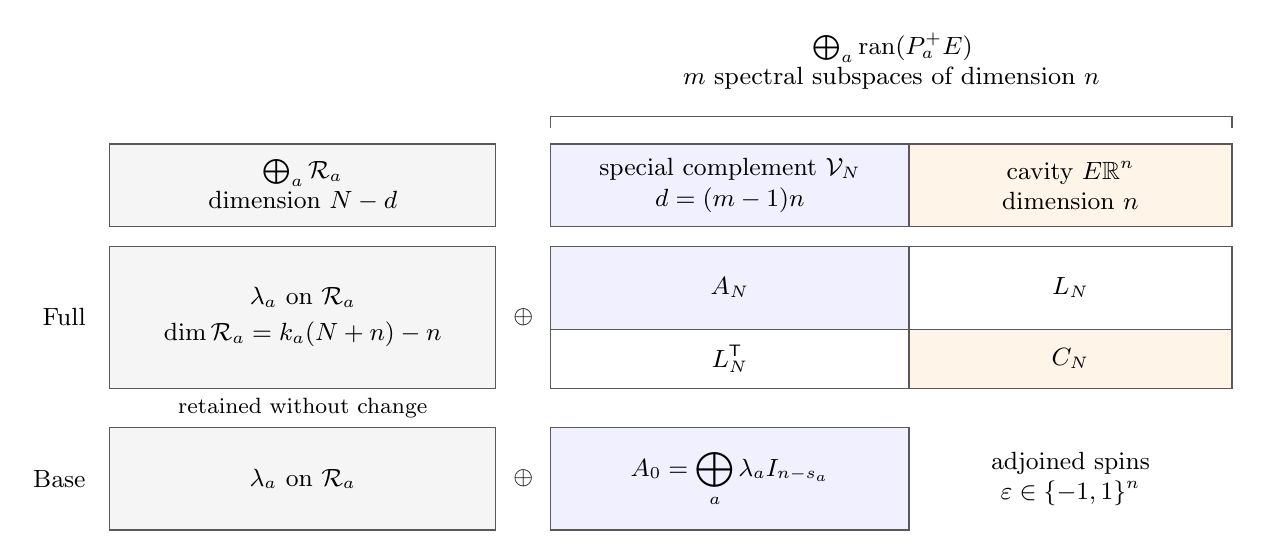
\begin{tikzpicture}[
  x=1cm,y=1cm,
  every node/.style={font=\small,align=center,inner sep=2pt},
  box/.style={draw=black!65,line width=.45pt},
  retained/.style={box,fill=black!4},
  special/.style={box,fill=blue!6},
  cavity/.style={box,fill=orange!9}
]
  \draw[black!65,line width=.45pt]
    (6.85,5.30)--(6.85,5.45)--(15.50,5.45)--(15.50,5.30);
  \node[text width=8.3cm] at (11.175,6.15)
    {$\textstyle\bigoplus_a\operatorname{ran}(P_a^+E)$\\
     $m$ spectral subspaces of dimension $n$};

  \draw[retained] (1.25,4.05) rectangle (6.15,5.10);
  \node at (3.70,4.575)
    {$\textstyle\bigoplus_a\mathcal R_a$\\dimension $N-d$};
  \draw[special] (6.85,4.05) rectangle (11.40,5.10);
  \node at (9.125,4.575)
    {special complement $\mathcal V_N$\\$d=(m-1)n$};
  \draw[cavity] (11.40,4.05) rectangle (15.50,5.10);
  \node at (13.45,4.575)
    {cavity $E\mathbb R^n$\\dimension $n$};

  \node[anchor=east] at (1.02,2.90) {Full};
  \draw[retained] (1.25,2.00) rectangle (6.15,3.80);
  \node at (3.70,2.90)
    {$\lambda_a$ on $\mathcal R_a$\\[2pt]
     $\dim\mathcal R_a=k_a(N+n)-n$};
  \node at (6.50,2.90) {$\oplus$};
  \draw[special] (6.85,2.75) rectangle (11.40,3.80);
  \draw[box] (11.40,2.75) rectangle (15.50,3.80);
  \draw[box] (6.85,2.00) rectangle (11.40,2.75);
  \draw[cavity] (11.40,2.00) rectangle (15.50,2.75);
  \node at (9.125,3.275) {$A_N$};
  \node at (13.45,3.275) {$L_N$};
  \node at (9.125,2.375) {$L_N^{\mathsf T}$};
  \node at (13.45,2.375) {$C_N$};

  \node[font=\footnotesize,inner sep=.5pt] at (3.70,1.75) {retained without change};
  \node[anchor=east] at (1.02,.85) {Base};
  \draw[retained] (1.25,.20) rectangle (6.15,1.50);
  \node at (3.70,.85) {$\lambda_a$ on $\mathcal R_a$};
  \node at (6.50,.85) {$\oplus$};
  \draw[special] (6.85,.20) rectangle (11.40,1.50);
  \node at (9.125,.85)
    {$\displaystyle A_0=\bigoplus_a\lambda_a I_{n-s_a}$};
  \node at (13.45,.85)
    {adjoined spins\\$\varepsilon\in\{-1,1\}^n$};
\end{tikzpicture}
\caption{The coupled cavity decomposition, with schematic block widths.
The full and base interactions agree on the remaining spectral spaces
$\mathcal R_a$. The span of the $m$ spectral images of the cavity
coordinates splits into the special complement and the cavity itself;
the full interaction on this span has each eigenvalue $\lambda_a$
with multiplicity $n$. Assigning $A_0$ to the special complement gives
the prescribed base multiplicities. When $m=1$, the special complement
is absent. Conditional on the base spectral projectors, the $n-s_a$
special axes assigned to group $a$ form a
uniform orthonormal frame. The base perturbations are generated
independently of these frames conditional on those projectors.}
\label{fig:cavity-decomposition}
\end{figure}


\subsection{Perturbations and bounded Gibbs tests}

The logarithmic comparison will give a lower bound involving one field
in the supremum defining $S$.  The cavity-spin tests will show that this
field is maximizing.

In averages containing $\varepsilon$, use its independent uniform
probability on the cavity cube.  Write $\langle\cdot\rangle_0$ for
this probability times the perturbed base Gibbs probability.  All
expectations below include the coupled spectral data and the special
frames.  Let $W$ denote \eqref{cav:factor} with the limiting matrices.

\begin{lemma}[Finite-size comparison]\label{cav:comparison}
There are deterministic $\delta_N\downarrow0$, uniform over the
perturbation parameters, such that
\begin{equation}\label{cav:increment-comparison}
 \mathcal F_{N+n}(\theta)-\mathcal F_N(\theta)
 \ge
 \E\log\big\langle
 W_N(y,\varepsilon)e^{-\delta_N(1+|y|^2)}
 \big\rangle_0.
\end{equation}
The right-hand side is bounded below uniformly in $N$ and $\theta$.
In addition, any bounded continuous test of the two-replica total
overlap and the cavity spins in the full system can be evaluated,
up to an error that vanishes first as $N\to\infty$ and then as
$B\to\infty$, using the base probability reweighted by
$W_N\ind_{\{|y|\le B\}}$ and the base total overlap.
\end{lemma}

\begin{proof}
We condition first on all coupled spectral data.  Outside the
special/cavity coordinates the full and base projectors coincide.
Their overlap difference, including the change of dimension divisor,
is bounded on two configurations by
\begin{equation}\label{cav:overlap-error}
 \frac{C_n}{N}\big(1+|y^1|^2+|y^2|^2\big).
\end{equation}
Multiplying by $Ne_N$ for the deterministic perturbations or by
$Ne_N^2$ for their Gaussian covariances gives a vanishing coefficient.
The changes in these amplitudes for a bounded jump of dimensions also
tend to zero.  The omitted Gaussian kernels and their derivatives
remain summable with the geometric weights.  Thus the deterministic
perturbation difference is bounded by
$o(1)(1+|y|^2)$, and the covariance difference by
$o(1)(1+|y^1|^2+|y^2|^2)$, uniformly in the parameters.

To see the sign of the comparison, put $g(\sigma)=1+|y|^2$.
Let $D_0,D_+$ be the deterministic base and full perturbations on
$(\sigma,\varepsilon)$, and let $\mathcal C_0,\mathcal C_+$ be the
corresponding Gaussian perturbation covariance kernels, conditional on
the coupled spectral data.
The preceding estimates give deterministic $a_N,b_N\to0$, uniform
in the parameters and spectral data, such that
\[
 |D_+-D_0|\le a_Ng,\qquad
 |(\mathcal C_+-\mathcal C_0)(1,2)|
       \le b_N(g(\sigma^1)+g(\sigma^2)).
\]
Choose independent centered Gaussian fields $X_0,X_+$ with these
conditional covariances.  Keep the full main interaction fixed and add
the interpolating perturbation
\[
 (1-\tau)D_0+\tau D_+
 +\sqrt{1-\tau}\,X_0+\sqrt\tau\,X_+
 -(1-\tau)\delta_Ng,\qquad 0\le\tau\le1.
\]
Write $Z_\tau$ and $\langle\cdot\rangle_\tau^{\mathrm{int}}$ for its partition
function and Gibbs probability.  The diagonal and pair terms in
Lemma~\ref{arr:gaussian-calculus} are each bounded below by
$-b_N\E\langle g\rangle_\tau^{\mathrm{int}}$.  Consequently
\[
 \frac{d}{d\tau}\E\log Z_\tau
 \ge(\delta_N-a_N-2b_N)\E\langle g\rangle_\tau^{\mathrm{int}}\ge0
\]
if $\delta_N\downarrow0$ is chosen to dominate $a_N+2b_N$.
At $\tau=0$ the partition function is
$Z_N^\theta\langle W_Ne^{-\delta_Ng}\rangle_0$;
at $\tau=1$ it is $Z_{N+n}^\theta$.  Integrating proves
\eqref{cav:increment-comparison}.  The block matrices are
uniformly bounded, so Jensen's inequality bounds its right-hand side
below by $-C\E\langle1+|y|^2\rangle_0$.  Lemma~\ref{cav:coupling}
gives the claimed uniform lower bound.

For the test comparison, choose $c>0$ smaller than every $\rho_a$.
The event $\min_a\lambda_{\min}(M_a)<c$ has probability tending to
zero and can be discarded in bounded tests.  On its complement, the
orthonormal coordinates of the projection onto
$\bigoplus_a\operatorname{ran}(P_a^+E)$ give
\[
 |y|^2+n
 =\sum_a\big|M_a^{-1/2}E^{\mathsf T}P_a^+\sigma^+\big|^2
 \le c^{-1}\sum_a|E^{\mathsf T}P_a^+\sigma^+|^2,
 \qquad \sigma^+=(\sigma,\varepsilon).
\]
At each fixed parameter choice the full disorder law is invariant
under site permutations.  For each site $j$,
\[
 \E\langle(P_a^+\sigma^+)_j^2\rangle_+
 =\frac1{N+n}\E\langle\|P_a^+\sigma^+\|^2\rangle_+
 \le1.
\]
Consequently
\begin{equation}\label{cav:full-tail}
 \limsup_{N\to\infty}\E\langle\ind_{\{|y|>B\}}\rangle_+
 \le\frac{C}{B^2}.
\end{equation}
This use of symmetry precedes the restriction; no symmetry of the
restricted Gibbs probability is needed.  Nor is an inverse moment of
$M_a$ required on the discarded event.

For fixed $B$, the restriction $|y|\le B$ is a fixed set once the
spectral data have been conditioned on.  It is nonempty for $B^2>d$,
since uniform base-spin sampling has mean squared projection $d$.
The perturbation differences on that set are bounded by
$O((a_N+b_N)(1+B^2))$.  Use the same interpolation without its penalty,
normalizing the Gibbs probability on this fixed restriction at every
$\tau$.
Lemma~\ref{arr:gaussian-calculus} bounds the change in the expected
bounded Gibbs test by $O((a_N+b_N)(1+B^2))=o(1)$ for fixed $B$.
At the base endpoint its probability is precisely the base
probability tilted by $W_N\ind_{\{|y|\le B\}}$.  Finally,
$|Q_{12}^+-Q_{12}|\le2n/(N+n)$, so uniform continuity permits replacing
the full total overlap by the base one.  Equation~\eqref{cav:full-tail}
then removes the restriction in the stated order.
\end{proof}

\subsection{Gaussian limits with explicit cutoffs}

The finite-size comparison has not asserted convergence of an
unbounded exponential factor.  We now pass to overlap limits with
cutoffs in place.  The subsequent quadratic calculation will supply
the uniform estimates needed to remove those cutoffs.

Take $\theta_N\in\mathcal G_N$ and a subsequence with limiting total
overlap quantile $p$.  By Proposition~\ref{rot:paths}, the Gaussian
marks supplied by Lemma~\ref{cav:coupling} have the covariance path
associated with
\begin{equation}\label{cav:H}
 H(x)=(b(x)I_d-A_0)^{-1},\qquad H(0)=0:
\end{equation}
their off-diagonal covariance at quantile coordinate $s$ and their
diagonal covariance are, respectively,
\begin{equation}\label{cav:path-convention}
 \int_0^{p(s)}H'(D_p(r))\,dr,
 \qquad
 \int_0^1H'(D_p(r))\,dr.
\end{equation}
Indeed each diagonal entry of $H$ is $f_a/\rho_a$ for its assigned
group.  The derivative $H'$ is positive semidefinite, so these paths
have nonnegative covariance increments and a nonnegative diagonal
excess.  If the top overlap equals one, that excess is zero.

Both the logarithmic increment and the cavity-spin tests must pass to
these Gaussian marks.  We keep separate cutoffs for the two quantities
until we have controlled the marks under the full cavity reweighting.

Choose finite-valued nondecreasing maps converging uniformly to the identity
on $[0,1]$, and let $\bar p$ be the resulting value roundings of $p$.
The rounded overlap arrays are exactly the finite cascades of
Lemma~\ref{arr:rpc-gg}.  On each such cascade use Gaussian
marks with \eqref{cav:path-convention} recalculated with $\bar p$.
The functions $H,H'$ are smooth on $[0,1]$ for the present finite
alphabet, and $D_{\bar p}\to D_p$ uniformly.  The recalculated
covariances therefore converge uniformly to the required ones.
Finite-replica Gaussian laws converge, including all the overlap
labels, by Lemma~\ref{arr:finite-replica}.

For the logarithmic lower bound, cap the factor in
\eqref{cav:increment-comparison} above at $e^T$, with $T>0$ fixed,
and first replace the logarithm of its integral by the logarithm of
that integral plus a floor $\epsilon>0$.  This is a bounded continuous
function of a bounded integral.  Polynomial approximation and extra
replicas give its limit as $N\to\infty$, then its finite-cascade
approximation as $\bar p\to p$.  The vanishing penalty and
\eqref{cav:blocks} do not change that limit: they converge uniformly
on compact sets of $y$, whose complements have vanishing probability
by \eqref{cav:base-moments}.

The floor can now be removed uniformly.  If $Z_{N,T}$ is the capped
base integral, Jensen's inequality and the bounded block matrices
give
\begin{equation}\label{cav:negative-log}
 (\log Z_{N,T})_-
 \le C\langle1+|y|^2\rangle_0,
 \qquad
 \sup_N\E[(\log Z_{N,T})_-^2]<\infty.
\end{equation}
The same bound holds for the limiting Gaussian calculations and all
finite-cascade approximations.  Splitting according as
$-\log Z_{N,T}$ is larger than a fixed number, and then increasing
that number, proves that adding the floor changes the expected
logarithm by a quantity tending uniformly to zero as
$\epsilon\downarrow0$.

For the restricted tests, fix $B>0$ and let
$q_{N,B}=\langle\ind_{\{|y|>B\}}\rangle_0$.  The base moment bound
and Markov's inequality give
\begin{equation}\label{cav:normalizer}
 \Prob(q_{N,B}>1/2)\le\frac{C}{B^2},
 \qquad
 \big\langle W_N\ind_{\{|y|\le B\}}\big\rangle_0
 \ge\frac12e^{-C(1+B^2)}
 \quad\text{if }q_{N,B}\le1/2.
\end{equation}
The same estimates hold in the finite cascades.  Thus denominator
powers in a bounded replica test may first be regularized, with an
arbitrarily small error apart from $C/B^2$, and then approximated by
polynomials using extra replicas.  The sphere $|y|=B>0$ has zero
probability for a centered Gaussian law, even when its covariance is
singular.  This justifies the restricted finite-replica passage.

The order is now explicit.  At fixed cap or radius and positive
regularizer, take the base-system limit and then refine the finite
rounding.  Remove the regularizer using
\eqref{cav:negative-log} or \eqref{cav:normalizer}.  It remains to
remove the cap and the radius in the finite-cascade calculations with
errors uniform in the rounding.  This last step requires the actual
quadratic transformation, to which we turn next.

\subsection{Quadratic Gaussian reweighting}

The quadratic part of the cavity factor changes the covariance of its
Gaussian marks.  The following lemma computes that change while keeping
track of the expected logarithm of the normalizing factor.  In particular,
the matrices in the quadratic factor need not commute.

\begin{lemma}[Quadratic tilt of a Gaussian cascade]\label{cav:quadratic}
Let $\mu=\sum_{a=1}^m\rho_a\delta_{\lambda_a}$, where
$\rho_a>0$ and $\sum_a\rho_a=1$, and put
$\lambda_+=\max_a\lambda_a$.  For $0<x\leq1$, let $b(x)>\lambda_+$
be the solution of $\sum_a\rho_a/(b(x)-\lambda_a)=x$.
Let $A_0,A$ be symmetric $d\times d$ matrices whose eigenvalues are at
most $\lambda_+$, and define
\begin{equation}\label{cav:q-def}
 K=A-A_0,\qquad H(x)=(b(x)\Id-A_0)^{-1}\quad(x>0),\qquad H(0)=0.
\end{equation}
Let $p\in\cP$ be constant with value $p_i$ on intervals of lengths
$w_i>0$, for $0\leq i<k$, where
$0\leq p_0\leq\cdots\leq p_{k-1}\leq1$ and $\sum_iw_i=1$.
Set $\zeta_i=\sum_{j<i}w_j$, so that $\zeta_0=0$ and $\zeta_k=1$.

On the corresponding Ruelle probability cascade, construct the marks
from centered Gaussian increments independent of one another and of the
unmarked cascade, with off-diagonal covariance path and diagonal covariance
\begin{equation}\label{cav:q-path}
 Q_H(s)=\int_0^{p(s)}H'(D_p(r))\,dr,
 \qquad V_H=\int_0^1H'(D_p(r))\,dr.
\end{equation}
Here the covariance shared by two sampled paths whose last common level
is $i$ is $Q_H(s)$ for $s$ in interval $i$.  Any diagonal excess is an
independent Gaussian residual, integrated separately at each visit to a
leaf.  More explicitly, write $v_\alpha$ for the cascade weights and
$y_\alpha$ for the sum of the common and branching Gaussian increments.
If $\gamma_\Sigma$ denotes the centered Gaussian probability measure
with covariance $\Sigma$, set
\[
 Z_K=\sum_\alpha v_\alpha
       \int\exp\left(\frac12(y_\alpha+z)^{\mathsf T}
                              K(y_\alpha+z)\right)
              \gamma_{V_H-Q_H(1-)}(dz).
\]
Then $Z_K$ is positive and finite almost surely, its logarithm is
integrable, and
\begin{equation}\label{cav:q-log}
 \E\log Z_K
 =-\frac12\int_0^1
   \left.\frac{d}{dx}\log\det(\Id-H(x)K)\right|_{x=D_p(r)}\,dr.
\end{equation}

After normalizing this quadratic tilt and relabeling the tree, the
cascade weights have their original law.  The terminal marks can be
represented by independent Gaussian increments, independent of the
unmarked cascade, with the covariance convention \eqref{cav:q-path}
using
\begin{equation}\label{cav:q-transform}
 \widetilde H(x)=(\Id-H(x)K)^{-1}H(x)
               =(b(x)\Id-A)^{-1}\quad(x>0),
 \qquad \widetilde H(0)=0
\end{equation}
in place of $H$.  This representation includes the tilted residual
draws and hence applies to joint sampling of any finite number of
terminal marks.  The derivatives and integrands at zero in these
formulas mean their smooth limits.  For $d=0$, determinants equal one
and all Gaussian marks are the unique vector in $\R^0$.
\end{lemma}

\begin{proof}
We first verify the conditional Gaussian integrals needed by the cascade
change of measure.  We then compute the normalizing constants and the
covariances under its tilted kernels.  The case $d=0$ is immediate, so
assume $d\geq1$.

The finite alphabet makes $b(x)$ well defined above $\lambda_+$.
Writing $u=1/b$ near $x=0$ changes its defining equation to
$x=\sum_a\rho_a u/(1-\lambda_a u)$, whose derivative in $u$ at zero
is one.  Consequently $H$ and $\widetilde H$ extend smoothly to zero,
with $H'(0)=\widetilde H'(0)=\Id$.  For positive $x$, put
$M_2(x)=\sum_a\rho_a/(b(x)-\lambda_a)^2$.  Differentiation gives
$b'(x)=-1/M_2(x)$ and
$H'(x)=M_2(x)^{-1}(b(x)\Id-A_0)^{-2}\succeq0$.
In particular, all covariance increments in \eqref{cav:q-path}
are well defined and positive semidefinite.

Append $p_k=1$ and put $p_{-1}=0$.  For $0\leq i\leq k$, define
\begin{equation}\label{cav:q-increments}
 \Sigma_i=\int_{p_{i-1}}^{p_i}H'(D_p(r))\,dr,
 \qquad H_i=H(D_p(p_i)),\qquad
 J_i=(\Id-H_iK)^{-1},\qquad K_i=KJ_i.
\end{equation}
The inverse defining $J_i$ exists: at positive arguments,
$H_i^{-1}-K=b(D_p(p_i))\Id-A\succ0$, and at zero $H_i=0$.
Also $K_i=(\Id-KH_i)^{-1}K$ is symmetric.
The increment $\Sigma_0$ is common to all leaves, increments
$\Sigma_i$ for $1\leq i<k$ are attached independently to the edges
at level $i$, and $\Sigma_k$ is the residual.  Since $D_p$ has slope
$-\zeta_i$ on $(p_{i-1},p_i)$ for $i>0$, while it is constant
on $(0,p_0)$, we have
\begin{equation}\label{cav:q-levels}
 H_k=0,\qquad
 H_{i-1}-H_i=\zeta_i\Sigma_i\quad(1\leq i\leq k),
 \qquad
 \Sigma_0=p_0H'(D_p(p_0)).
\end{equation}
These identities also hold when some adjacent overlap values coincide.

For $i>0$, write $\Delta_i=\zeta_i\Sigma_i$.  The matrix ordering
in the following identity will be important:
\begin{equation}\label{cav:q-factor}
 \Id-\Delta_iK_i=(\Id-H_{i-1}K)J_i,
 \qquad
 \det(\Id-\Delta_iK_i)
   =\frac{\det(\Id-H_{i-1}K)}{\det(\Id-H_iK)}.
\end{equation}
The symmetric Gaussian precision matrix satisfies
\begin{equation}\label{cav:q-precision}
 \Id-\zeta_i\Sigma_i^{1/2}K_i\Sigma_i^{1/2}\succ0.
\end{equation}
To prove this, replace $\Delta_i$ in \eqref{cav:q-factor} by
$t\Delta_i$, $0\leq t\leq1$, and set $S_t=H_i+t\Delta_i$.
If $H_{i-1}=0$, then $\Sigma_i=0$ and the claim is immediate.
Otherwise $H_{i-1}\succ0$, and each nonzero $S_t$ is positive
definite and at most $H_{i-1}$.  Thus
\[
 S_t^{-1}-K\succeq H_{i-1}^{-1}-K\succ0.
\]
It follows that $\det(\Id-S_tK)\ne0$; this is also true when
$S_t=0$.  By \eqref{cav:q-factor} and the identity
$\det(\Id-BC)=\det(\Id-CB)$, the symmetric matrix in
\eqref{cav:q-precision}, with $\zeta_i$ replaced by $t\zeta_i$,
never has a zero eigenvalue.  At $t=0$ it is the identity, proving
\eqref{cav:q-precision} by continuity.

For a vector $u\in\R^d$, completion of the square now gives the
finite integral
\begin{equation}\label{cav:q-gaussian-integral}
 \frac1{\zeta_i}\log\int
       \exp\left(\frac{\zeta_i}{2}
                    (u+z)^{\mathsf T}K_i(u+z)\right)
                    \gamma_{\Sigma_i}(dz)
 =-\frac1{2\zeta_i}\log\det(\Id-\Delta_iK_i)
       +\frac12u^{\mathsf T}K_{i-1}u.
\end{equation}
Indeed, if $T_i=(\Id-\Delta_iK_i)^{-1}$, then
\eqref{cav:q-factor} implies $J_iT_i=J_{i-1}$ and hence
$K_iT_i=K_{i-1}$.  Formula \eqref{cav:q-gaussian-integral} also
holds for singular $\Sigma_i$, by writing $z=\Sigma_i^{1/2}g$
with $g$ a standard Gaussian vector.

Starting at $K_k=K$, backward integration therefore produces the
quadratic coefficients $K_i$ of \eqref{cav:q-increments}.
For $1\leq i<k$, \eqref{cav:q-gaussian-integral} verifies exactly
the conditional fractional exponential moment of exponent $\zeta_i$
required by the marked-cascade change of measure in Proposition~\ref{arr:rpc}.
The residual step $i=k$ uses exponent $\zeta_k=1$ and verifies its
ordinary exponential moment.  The root uses exponent zero, namely
ordinary expectation of the backward value; its quadratic contribution
is $\Tr(\Sigma_0K_0)/2$.  Since a Gaussian quadratic polynomial is
integrable, no exponential moment of the root quadratic term is needed.
The same recursion and Proposition~\ref{arr:rpc}, conditional on the root
mark, show that $Z_K$ is positive and finite almost surely.  Their
logarithmic integrability assertion applies because the Gaussian
integrals above have finite constants and the root value is a quadratic
polynomial in a finite-dimensional Gaussian vector.  Thus
\begin{equation}\label{cav:q-constants}
 \E\log Z_K
 =\frac12\Tr(\Sigma_0K_0)
 -\sum_{i=1}^k\frac1{2\zeta_i}
   \log\frac{\det(\Id-H_{i-1}K)}{\det(\Id-H_iK)}.
\end{equation}
Set $f(x)=\log\det(\Id-H(x)K)$.  Its derivative is
$f'(x)=-\Tr(H'(x)K(\Id-H(x)K)^{-1})$.
On $(0,p_0)$ this identifies the root term in
\eqref{cav:q-constants} with $-\frac12\int_0^{p_0}f'(D_p(r))\,dr$.
On every subsequent interval, the change of variable
$D_p'(r)=-\zeta_i$ identifies its determinant term with the
corresponding integral.  Summing proves \eqref{cav:q-log}.

It remains to identify the terminal marks under the quadratic tilt.
The marked-cascade rule leaves the root law unchanged and gives, at
step $i>0$, the Gaussian kernel obtained by multiplying the density
of $z\sim\gamma_{\Sigma_i}$ by
$\exp(\zeta_i(u+z)^{\mathsf T}K_i(u+z)/2)$ and normalizing.
If $Y_{i-1}=u$ is the running sum before this step, square completion
gives
\begin{equation}\label{cav:q-kernels}
 \E[Y_i\mid Y_{i-1}]=T_iY_{i-1},\qquad
 \Cov(Y_i\mid Y_{i-1})=T_i\Sigma_i,
 \qquad T_i=(\Id-\Delta_iK_i)^{-1}.
\end{equation}
The covariance is symmetric and positive semidefinite, since it equals
\[
 \Sigma_i^{1/2}
 (\Id-\zeta_i\Sigma_i^{1/2}K_i\Sigma_i^{1/2})^{-1}
 \Sigma_i^{1/2}.
\]
The conditional covariance is independent of the preceding value, and
the kernels on distinct child edges are conditionally independent.

Rescale the running sums by $U_i=J_iY_i$.  Because
$J_iT_i=J_{i-1}$, the process $U_i$ has centered independent
innovations on the tree.  Their covariances, and that of the common
root, are respectively
\begin{equation}\label{cav:q-innovations}
 \Cov(U_i-U_{i-1})=J_{i-1}\Sigma_iJ_i^{\mathsf T}\quad(i>0),
 \qquad \Cov(U_0)=J_0\Sigma_0J_0^{\mathsf T}.
\end{equation}
For symmetric matrices $B,C$ for which the indicated inverses exist,
the map $F(B)=(\Id-BK)^{-1}B$ satisfies
\begin{equation}\label{cav:q-resolvent-difference}
 F(B)-F(C)
 =(\Id-BK)^{-1}(B-C)(\Id-KC)^{-1}.
\end{equation}
This follows by multiplying on the left by $\Id-BK$ and on the
right by $\Id-KC$.  Applying it to $B=H_{i-1}$ and $C=H_i$
in \eqref{cav:q-innovations} shows that the covariance at step $i>0$
is
\[
 \frac{\widetilde H(D_p(p_{i-1}))-
       \widetilde H(D_p(p_i))}{\zeta_i}
 =\int_{p_{i-1}}^{p_i}\widetilde H'(D_p(r))\,dr.
\]
Here \eqref{cav:q-transform} follows directly from
$H(x)^{-1}-K=b(x)\Id-A$ at positive $x$.
Differentiating \eqref{cav:q-resolvent-difference} along $H(x)$
also gives
\begin{equation}\label{cav:q-root-covariance}
 \widetilde H'(x)=J(x)H'(x)J(x)^{\mathsf T},\qquad
 J(x)=(\Id-H(x)K)^{-1},
\end{equation}
so the root covariance in \eqref{cav:q-innovations} is
$p_0\widetilde H'(D_p(p_0))$, as required.
Since $J_k=\Id$, the final sum $U_k$ equals the original terminal
mark $Y_k$.  The cascade change of measure gives the original unmarked
cascade law independently of these Gaussian innovations, completing
the claimed representation.

All the endpoint cases are included.  If $p_{k-1}=1$, then
$\Sigma_k=0$ and the residual step makes no change.  If $p=1$
everywhere, then $D_p=0$, $J_i=\Id$, and $\Sigma_0=\Id$;
the sole quadratic contribution is the ordinary root expectation
$\Tr(K)/2$.  Equal adjacent overlap values simply give zero
increments in the same formulas.
\end{proof}

\subsection{Removing cutoffs and evaluating the increment}

Apply Lemma~\ref{cav:quadratic} to the matrices supplied by
Lemma~\ref{cav:coupling}.  The eigenvalues of $A$ and $A_0$ are at most
$\lambda_+$: $A$ is a compression of
$\bigoplus_a\lambda_a I_n$, and $A_0$ has the specified spectral
alphabet.  The lemma therefore applies to every finite rounding
$\bar p$.  Its joint Gaussian representation will bound the two-replica
moment arising from the remaining linear tilt.  That bound removes both
cutoffs uniformly in the rounding, after which we compute the increment
and the spin tests.

For a finite step quantile $q$, denote the cascade prior with the
Gaussian covariance convention \eqref{cav:path-convention}, including
the independent residual and uniform cavity spins, by
$\langle\cdot\rangle_q$.  Write
$\langle\cdot\rangle_{q,W}$ for its normalized tilt by
$W(y,\varepsilon)$.

\begin{lemma}[Uniform removal of cutoffs]\label{cav:cutoffs}
For the fixed finite alphabet and fixed $n$, and every $r>0$,
\begin{equation}\label{cav:tilted-moments}
 \sup_{q\ \mathrm{finite\ step}}
 \E\langle |y|^r\rangle_{q,W}<\infty.
\end{equation}
Consequently the error in the expected logarithm from replacing $W$
by $\min(W,e^T)$ tends uniformly to zero as $T\to\infty$.  The error
in a bounded replica test from restricting to $|y|\le B$ tends
uniformly to zero as $B\to\infty$, with any fixed bounded convention
if the restricted normalizer is zero.
\end{lemma}

\begin{proof}
First perform only the quadratic tilt.  By
Lemma~\ref{cav:quadratic}, the terminal marks then have a Gaussian
cascade representation associated with
$\widetilde H(x)=(b(x)I_d-A)^{-1}$.  Its diagonal covariance is
\[
 \int_0^1\widetilde H'(D_q(r))\,dr,
\]
whose norm is bounded by $\sup_{0\le x\le1}\|\widetilde H'(x)\|$.
This is finite for the fixed alphabet, independently of the number of
steps and their weights.  Indeed $b(x)>\lambda_+$ for $x>0$, and the
inverse has the smooth extension at zero already proved in the lemma.

Let $\langle\cdot\rangle_{q,K}$ denote the normalized quadratic
tilt, still including the uniform cavity-spin probability.  The
remaining exponent is
\[
 V(y,\varepsilon)=y^{\mathsf T}L\varepsilon
                  +\frac12\varepsilon^{\mathsf T}C\varepsilon.
\]
For each realization, Jensen's inequality gives
$\langle e^V\rangle_{q,K}^{-1}\le\langle e^{-V}\rangle_{q,K}$.
Taking two replicas therefore gives
\begin{equation}\label{cav:linear-moment-bound}
 \E\langle|y|^r\rangle_{q,W}
 \le\E\big\langle |y^1|^r e^{V(y^1,\varepsilon^1)
                                      -V(y^2,\varepsilon^2)}
                \big\rangle_{q,K}.
\end{equation}
Conditional on their branching, the two marks on the right are
centered joint Gaussians with uniformly bounded covariance.  The spin
coefficients range over a fixed finite set.  Gaussian
polynomial-exponential moments thus bound the right side uniformly,
proving \eqref{cav:tilted-moments}.  This argument includes the
residual draws as part of the probability prior.  Jensen's inequality
and the same exponential-linear moments also show that the remaining
logarithmic normalizer is integrable.

Put $g_T=(\log W-T)_+$.  Since
$\min(W,e^T)=We^{-g_T}$,
\[
 0\le\log\langle W\rangle_q
       -\log\langle\min(W,e^T)\rangle_q
 \le\langle g_T\rangle_{q,W}.
\]
The bound $|\log W|\le C(1+|y|^2)$ and
\eqref{cav:tilted-moments} make its expectation tend uniformly to zero.
Restriction of an $l$-replica bounded test changes its expectation by
at most a constant times $l\langle\ind_{\{|y|>B\}}\rangle_{q,W}$.
Markov's inequality and \eqref{cav:tilted-moments} prove the second
assertion, including the event where the restricted normalizer is zero.
\end{proof}

For $p\in\cP$, define
\begin{equation}\label{cav:field-path}
 h_p(s)=\int_0^{p(s)}R'(D_p(r))\,dr.
\end{equation}
This is a bounded nonnegative nondecreasing path.  For $x>0$,
\[
 R'(x)=\frac1{x^2}-\frac1{M_2(x)}\ge0,
 \qquad M_2(x)=\sum_a\frac{\rho_a}{(b(x)-\lambda_a)^2}\ge x^2,
\]
and the derivative has its smooth nonnegative limit at zero.  If $p$
is a finite step quantile, then $h_p\in\cH$.

\begin{proposition}[Evaluation of the cavity factor]\label{cav:evaluation}
For every finite step quantile $p$, the cascade factor constructed above
satisfies
\begin{equation}\label{cav:evaluated}
 \frac1n\E\log\langle W\rangle_p
 =\ell(h_p)+\frac12\int_0^1p(s)h_p(s)\,ds+G_1(p).
\end{equation}
For a fixed cavity site $j$ and a bounded continuous function $\phi$,
the same tilted calculation satisfies
\begin{equation}\label{cav:spin-test}
 \E\langle\phi(Q_{12})\varepsilon_j^1\varepsilon_j^2\rangle_{p,W}
 =\int_0^1\phi(p(s))B_{h_p}(s)\,ds,
\end{equation}
where $Q_{12}$ is the common-level value prescribed by $p$ and
$B_{h_p}$ is the conditional two-spin product from
Proposition~\ref{fld:derivative}.  The common-level distribution itself
is unchanged by the tilt.
\end{proposition}

\begin{proof}
Compression of the resolvent of the limiting block matrix onto the
cavity coordinates gives, for $b=b(x)$,
\begin{equation}\label{cav:compression}
 \big(bI_n-C-L^{\mathsf T}(bI_d-A)^{-1}L\big)^{-1}
 =\sum_a\frac{\rho_a I_n}{b-\lambda_a}=xI_n.
\end{equation}
The whole block has eigenvalue $\lambda_a$ with multiplicity $n$.
Its Schur determinant and the multiplicities in $A_0$ give
\begin{align}
 C+L^{\mathsf T}\widetilde H(x)L&=R(x)I_n,
       \label{cav:scalar-field}\\
 \log\det(I_d-H(x)K)
 &=\log\frac{\det(bI_d-A)}{\det(bI_d-A_0)}\notag\\
 &=n\left(\log x+\sum_a\rho_a\log(b-\lambda_a)\right).
       \label{cav:determinant}
\end{align}
To see the multiplicities explicitly,
$\det(bI_d-A)=x^n\prod_a(b-\lambda_a)^n$ whereas
$\det(bI_d-A_0)=\prod_a(b-\lambda_a)^{n-s_a}$.
Differentiating \eqref{cav:determinant} and using
$\sum_a\rho_a/(b-\lambda_a)=x$ yields
\begin{equation}\label{cav:determinant-derivative}
 \frac1n\frac{d}{dx}\log\det(I_d-H(x)K)
 =\frac1x+xb'(x)=xR'(x).
\end{equation}

Differentiating \eqref{cav:scalar-field} gives
\[
 L^{\mathsf T}\widetilde H'(x)L=R'(x)I_n.
\]
Thus, after the quadratic transformation, the field $L^{\mathsf T}y$
has independent coordinates with common-level covariance path $h_p$.
Its diagonal covariance is
$vI_n$, where
\[
 v=\int_0^1R'(D_p(r))\,dr.
\]
Writing $h_*=h_p(1-)$, the independent residual has covariance
$(v-h_*)I_n$.  Since every cavity spin has squared norm $n$,
integrating this residual and the deterministic cavity term
$C=R(0)I_n$ contributes $n[R(0)+v-h_*]/2$ to the logarithm.
The remaining spin sum is $\prod_{j=1}^n\cosh z_j$ for the
nonresidual field $z$.  Its logarithm is additive over coordinates,
so the Gaussian backward recursion and its tilted kernels factor over
those coordinates.  This recursion contributes
$n[\ell(h_p)+h_*/2]$.  Lemma~\ref{cav:quadratic} and
\eqref{cav:determinant-derivative} therefore give
\begin{equation}\label{cav:before-parts}
 \frac1n\E\log\langle W\rangle_p
 =\ell(h_p)+\frac12\left[
 R(0)+\int_0^1(1-D_p(r))R'(D_p(r))\,dr\right].
\end{equation}
All three contributions include the root interval; the independent
residual was integrated at exponent one.

Fubini's theorem and the definition of $D_p$ give
\[
 \int_0^1p(s)h_p(s)\,ds
 =\int_0^1R'(D_p(r))\int_{\{s:p(s)>r\}}p(s)\,ds\,dr,
\]
and, almost everywhere in $r$,
\[
 1-D_p(r)-\int_{\{s:p(s)>r\}}p(s)\,ds=-rD_p'(r).
\]
Subtracting the pairing with $h_p$ from the bracket in
\eqref{cav:before-parts} thus gives
\[
 R(0)-\int_0^1r\,dR(D_p(r))
 =\int_0^1R(D_p(r))\,dr=2G_1(p),
\]
where $D_p(1)=0$ supplies the endpoint at one.  This proves
\eqref{cav:evaluated}.

Both the quadratic transformation and the remaining spin tilt use
the marked-cascade rule of Proposition~\ref{arr:rpc}.  Its tree
relabeling preserves all common-level values, and leaves their law
unchanged.  The scalar residual correction is independent of the
spins.  Conditional on a common level, the remaining single-coordinate
two-spin product is exactly $B_{h_p}$ from the Ising recursion; the
independent coordinates factor through its tilted kernels.  This
proves \eqref{cav:spin-test} and the last assertion.
\end{proof}

We can now finish the passage from finite size to the evaluated
increment.  For a good parameter sequence with limiting quantile $p$,
the capped comparison, finite-replica approximation, and
Lemma~\ref{cav:cutoffs} imply
\begin{equation}\label{cav:preliminary-lower}
 \liminf_{N\to\infty}
 \frac{\mathcal F_{N+n}(\theta_N)-\mathcal F_N(\theta_N)}{n}
 \ge\ell(h_p)+\frac12\int_0^1p(s)h_p(s)\,ds+G_1(p).
\end{equation}
Here $\ell(h_p)$ uses the bounded-path extension of
Theorem~\ref{fld:concavity}.  Indeed uniform rounding gives
$h_{\bar p}\to h_p$ uniformly, so the right side of
\eqref{cav:evaluated} converges by the $L^1$ continuity of $\ell$.
At each fixed logarithmic cap the limiting lower bound is the capped
finite-cascade value; its difference from the uncapped value tends
uniformly to zero by Lemma~\ref{cav:cutoffs}.  This verifies
\eqref{cav:preliminary-lower} in the cutoff order already specified,
without untruncated moment convergence at finite system size.

\subsection{The maximizing field and the lower bound}

The expression in \eqref{cav:preliminary-lower} contains one field,
whereas the proposed answer contains a supremum over fields.  To obtain
the required inequality, we must prove that this particular field
maximizes that supremum.  The information comes from cavity-spin tests,
not from the logarithmic comparison alone.

\begin{proposition}[Cavity self-consistency]\label{cav:self-consistency}
Let $p$ be a limiting total-overlap quantile along any sequence
$\theta_N\in\mathcal G_N$ used in
\eqref{cav:preliminary-lower}.  For value roundings $\bar p\to p$
as above,
\begin{equation}\label{cav:B-limit}
 B_{h_{\bar p}}\longrightarrow p\quad\text{in }L^1(0,1).
\end{equation}
Consequently
\begin{equation}\label{cav:supremum}
 S(p)=\ell(h_p)+\frac12\int_0^1p(s)h_p(s)\,ds.
\end{equation}
Thus $h_p$ attains the field supremum in the bounded-path completion.
\end{proposition}

\begin{proof}
For any fixed cavity site $j$, site permutation symmetry of the full
model gives, for every bounded continuous $\phi$,
\[
 \E\langle\phi(Q_{12}^+)\varepsilon_j^1\varepsilon_j^2\rangle_+
 =\E\langle\phi(Q_{12}^+)Q_{12}^+\rangle_+.
\]
Apply the restricted test comparison of Lemma~\ref{cav:comparison},
pass through the bounded finite-replica calculations, and then remove
the restriction using Lemma~\ref{cav:cutoffs}.  Proposition~\ref{cav:evaluation}
and preservation of the common-level law give
\begin{equation}\label{cav:test-identity}
 \lim_{\bar p\to p}\int_0^1
 \phi(\bar p(s))\big(B_{h_{\bar p}}(s)-\bar p(s)\big)\,ds=0.
\end{equation}
No GG property of the full system was used here: the base parameters
are good, while site symmetry holds for the full model at every fixed
parameter choice.

The functions $B_{h_{\bar p}}$ are nondecreasing and take values in
$[0,1]$, so they are relatively compact in $L^1$.  We explain why any
subsequential limit $B$ is a measurable function of $p$; this is needed
to infer equality from \eqref{cav:test-identity}.  Since each rounding
is a function of the values of $p$, it is constant on every plateau of
$p$.  The corresponding field levels are tied there.  Their zero
increments give identical conditional positions and magnetizations,
so $B_{h_{\bar p}}$ is also constant there, by
Proposition~\ref{fld:derivative}.  An $L^1$ limit preserves this property
on every positive-length plateau.  There are only countably many such
intervals.  Outside their interiors and their null set of endpoints,
the generalized inverse of the nondecreasing function $p$ recovers
the quantile coordinate.  Thus $B$ is measurable with respect to $p$
almost everywhere, including when $p$ has a singular-continuous part.

Passing to the limit in \eqref{cav:test-identity} shows that the signed
pushforward of $(B-p)\,ds$ under $p$ vanishes, since continuous tests
determine finite measures on $[0,1]$.  The established measurability
then gives $B=p$ almost everywhere.  Every subsequential limit is the
same, proving \eqref{cav:B-limit}.

For any fixed $v\in\cH$, take common refinements of its intervals and
those of $h_{\bar p}$.  The supporting inequality from
Theorem~\ref{fld:concavity}, including tied levels, is
\[
 \ell(v)\le\ell(h_{\bar p})
 -\frac12\int_0^1B_{h_{\bar p}}(s)
                    (v(s)-h_{\bar p}(s))\,ds.
\]
Letting $\bar p\to p$ proves that the supremum defining $S(p)$ is at
most the right side of \eqref{cav:supremum}.  Conversely,
$h_{\bar p}\in\cH$, and their values in the definition of $S(p)$,
with $p$ fixed in the pairing, converge to that same expression.
This proves \eqref{cav:supremum}.
\end{proof}

\begin{proposition}[Finite-alphabet lower bound]\label{cav:lower}
Let $\mu=\sum_{a=1}^m\rho_a\delta_{\lambda_a}$ have positive rational
proportions.  Fix $n$ with $n\rho_a\in\N$ for every $a$, and a
progression of dimensions and spectral counts satisfying
\eqref{cav:counts}.  Along this progression, the unperturbed pressure
satisfies
\[
 \liminf_{N\to\infty}\E P_N
 \ge\inf_{p\in\cP}\{S(p)+G_1(p)\}.
\]
\end{proposition}

\begin{proof}
Put $\mathcal V=\inf_{p\in\cP}\{S(p)+G_1(p)\}$.  This is finite:
$S\ge0$, $G_1$ is bounded, and the zero trial has finite $S$ by
Lemma~\ref{fld:domain}.  Every sequence of good base parameters has
a subsequence with the overlap limits used above.  Equations
\eqref{cav:preliminary-lower} and \eqref{cav:supremum} therefore imply
\[
 \liminf_{N\to\infty}\inf_{\theta\in\mathcal G_N}
 \big(\mathcal F_{N+n}(\theta)-\mathcal F_N(\theta)\big)
 \ge n\mathcal V.
\]
Indeed any failure would select a sequence of parameters whose
subsequential overlap limit contradicts the two equations.

Lemma~\ref{cav:comparison} gives a uniform lower bound for the
increments also outside $\mathcal G_N$.  Since
$\eta(\mathcal G_N)\to1$, integration over the common parameter
space yields
\[
 \liminf_{N\to\infty}\int
 \big(\mathcal F_{N+n}(\theta)-\mathcal F_N(\theta)\big)\,\eta(d\theta)
 \ge n\mathcal V.
\]
The parameter space includes the whole infinite sequence, with the
size-$N$ partition function ignoring later coordinates.  Hence these
integrated increments telescope exactly along the progression.
Dividing their sum by the terminal dimension proves the lower bound
for the parameter-averaged perturbed pressure.  The perturbations
change the expected log partition by $O(Ne_N)=o(N)$, uniformly in
parameters, so the same bound holds for $\E P_N$.
\end{proof}

The fixed-$n$ comparison is now complete.  Its constants may depend on
the finite alphabet and on $n$; no uniformity across later spectral
approximations was used.  Section~\ref{sec:general} will combine this
bound with the upper bound and remove the rational-count and
finite-alphabet restrictions.

\section{General spectral distributions}\label{sec:general}

The upper and lower bounds now determine the pressure for finite spectral
alphabets with rational proportions along the progressions used in the
cavity argument.  We first remove these arithmetic restrictions, and then
approximate an arbitrary compactly supported spectral law.  In this
section, subscripts in $R_\nu$ and $G_{t,\nu}$ specify the spectral law;
$\mathcal F(\nu)$ denotes the variational value in
\eqref{eq:variational} with that law.  The functions $S$ and $D_p$ do not
depend on the spectral law.

\subsection{Continuity of the spectral term}

The transform can reach the upper support edge, so its continuity must
include that branch of the definition.  The following statement needs
no regularity of the measure near the edge.

\begin{lemma}\label{gen:R-continuity}
Let $\nu_j$ and $\nu$ be probability measures supported in a common
interval $[-K,K]$.  Suppose that $\nu_j$ converges weakly to $\nu$ and
that
\[
 e_j:=\max\supp\nu_j\longrightarrow e:=\max\supp\nu.
\]
Define $b_{\nu_j}$ and $R_{\nu_j}$ by the edge convention of
Theorem~\ref{thm:main}, and likewise for $\nu$.  Then
\begin{equation}\label{gen:R-uniform}
 \sup_{0\le x\le1}|R_{\nu_j}(x)-R_\nu(x)|\longrightarrow0.
\end{equation}
Consequently,
\begin{equation}\label{gen:variational-continuity}
 |\mathcal F(\nu_j)-\mathcal F(\nu)|
 \le \frac12\sup_{0\le x\le1}|R_{\nu_j}(x)-R_\nu(x)|
 \longrightarrow0.
\end{equation}
\end{lemma}

\begin{proof}
For a measure $\tau$ with upper support edge $e_\tau$, put
\[
 H_\tau(z)=\int\frac{\tau(d\lambda)}{z-\lambda},
 \qquad z>e_\tau.
\]
This function is continuous and strictly decreasing.  Thus
$b_\tau(x)>e_\tau$ exactly when $x<H_\tau(e_\tau+)$, and in that
case $H_\tau(b_\tau(x))=x$.  In the remaining case
$b_\tau(x)=e_\tau$.  In both cases,
\begin{equation}\label{gen:b-bounds}
 e_\tau\le b_\tau(x)\le e_\tau+x^{-1},
 \qquad -K\le R_\tau(x)\le K.
\end{equation}
The first upper bound follows from
$H_\tau(z)\le(z-e_\tau)^{-1}$.  The lower bound on $R_\tau$
follows from $H_\tau(z)\ge(z+K)^{-1}$, using the edge limit of this
inequality when the transform is capped.

We first work away from zero.  Let $x_j\to x>0$ and pass to a
subsequence on which $b_{\nu_j}(x_j)\to b_*$.  The bounds
\eqref{gen:b-bounds} imply that such subsequences exist and that
$b_*\ge e$.  If $b_*>e$, the defining equations are uncapped for
large $j$.  Weak convergence, with their arguments uniformly separated
from the supports, gives
\[
 H_\nu(b_*)=x.
\]
Hence $b_*=b_\nu(x)$.  If $b_*=e$ but $b_\nu(x)>e$, choose
$c\in(e,b_\nu(x))$.  Then $H_\nu(c)>x$, so
$H_{\nu_j}(c)>x_j$ for large $j$.  Strict monotonicity, including the
definition of the capped branch, forces $b_{\nu_j}(x_j)>c$, a
contradiction.  These two cases prove
\[
 b_{\nu_j}(x_j)\longrightarrow b_\nu(x).
\]
The same argument with the measure fixed proves continuity of
$b_\nu$ on $(0,1]$.  A compactness argument now gives uniform
convergence of $R_{\nu_j}$ on every $[\varepsilon,1]$.

Near zero the convergence is uniform for a different reason.  If $K=0$
there is nothing to prove.  For $K>0$ and $x<(4K)^{-1}$, the transform
cannot be capped, since
$H_\tau(e_\tau+)\ge(2K)^{-1}$.  Write
$b_\tau(x)=x^{-1}+R_\tau(x)$ in its defining equation.  The bound
$|R_\tau|\le K$ permits the uniform expansion
\[
 1=\int\frac{\tau(d\lambda)}{1+x(R_\tau(x)-\lambda)}
  =1-x\left(R_\tau(x)-\int\lambda\,\tau(d\lambda)\right)
    +O(K^2x^2).
\]
Therefore
\begin{equation}\label{gen:R-at-zero}
 R_\tau(x)=\int\lambda\,\tau(d\lambda)+O(K^2x),
\end{equation}
with a constant independent of $\tau$.  Weak convergence on the common
bounded interval implies convergence of the means.  Combining
\eqref{gen:R-at-zero} with the convergence away from zero proves
\eqref{gen:R-uniform}.

Finally, $0\le D_p(r)\le1$ for every admissible $p$ and $r$, and hence
\[
 \sup_{p\in\cP}|G_{1,\nu_j}(p)-G_{1,\nu}(p)|
 \le\frac12\|R_{\nu_j}-R_\nu\|_\infty.
\]
Taking infima after adding the common functional $S$ proves
\eqref{gen:variational-continuity}.  These infima are finite: $S\ge0$
and $S(0)=0$ by Lemma~\ref{fld:domain}, whereas the transforms are
bounded by \eqref{gen:b-bounds}.
\end{proof}

\subsection{Spectral multiplicities and approximation}

For two diagonal spectra of the same size, using the same orthogonal
matrix gives the elementary comparison
\begin{equation}\label{gen:operator-comparison}
 |P_N(\Lambda,U)-P_N(\widetilde\Lambda,U)|
 \le\frac12\|\Lambda-\widetilde\Lambda\|_{\mathrm{op}}.
\end{equation}
It follows by comparing each spin energy and using $|\sigma|^2=N$.
The same argument gives monotonicity under coordinatewise increase of
the eigenvalues and the exact shift identity
\begin{equation}\label{gen:scalar-shift}
 P_N(\Lambda+c\Id,U)=P_N(\Lambda,U)+\frac c2.
\end{equation}
To change multiplicities, however, a small operator-norm error is not
available.  The next bound uses rotational symmetry inside each
eigenspace.

\begin{lemma}\label{gen:counts}
Fix distinct real numbers $\lambda_1,\ldots,\lambda_m$, and let
$L=\max_a\lambda_a-\min_a\lambda_a$.  Let $k_a$ and
$\widetilde k_a$ be positive integers whose sums are both $N$.
For diagonal matrices $\Lambda$ and $\widetilde\Lambda$ with these
multiplicities,
\begin{equation}\label{gen:count-comparison}
 \left|\E P_N(\Lambda,U)-\E P_N(\widetilde\Lambda,U)\right|
 \le\frac L2\max_a
 \frac{|k_a-\widetilde k_a|}{\min(k_a,\widetilde k_a)}.
\end{equation}
The same inequality holds for any fixed spin prior on the cube,
including a prior with deterministic external fields.
\end{lemma}

\begin{proof}
Arrange the two diagonal matrices so that, for each $a$,
$\min(k_a,\widetilde k_a)$ axes retain the value $\lambda_a$.
Haar invariance makes this rearrangement immaterial.  Set
$\Delta=\widetilde\Lambda-\Lambda$ and
\[
 f(s)=\E P_N(\Lambda+s\Delta,U),\qquad 0\le s\le1.
\]
Convexity of the log partition function gives
$f'(0)\le f(1)-f(0)\le f'(1)$.  At either endpoint,
\[
 f'(s)=\frac1{2N}\E\left\langle\sum_i\Delta_{ii}x_i^2
                  \right\rangle_s,
 \qquad x=U\sigma.
\]
Within a group of equal endpoint eigenvalues, the expected squared
projections are equal on all axes.  Indeed, rotating the corresponding
rows of $U$ preserves both its Haar law and the spin Hamiltonian; the
spin prior is unaffected.  If a group has $q_a$ axes and $c_a$ changed
axes, its changed axes therefore carry the fraction $c_a/q_a$ of the
group's expected squared spin norm.  Since $|\Delta_{ii}|\le L$ and
the total squared norm is $N$,
\[
 |f'(s)|\le\frac L2\max_a\frac{c_a}{q_a},
 \qquad s\in\{0,1\}.
\]
At the first endpoint $c_a=(k_a-\widetilde k_a)_+$, and at the second
$c_a=(\widetilde k_a-k_a)_+$.  The endpoint bounds prove
\eqref{gen:count-comparison}.
\end{proof}

\begin{proposition}\label{gen:approximation}
Let $\Lambda_N$ be deterministic diagonal matrices.  Suppose that their
empirical measures converge weakly to a compactly supported probability
measure $\mu$, and write
$a=\min\supp\mu$ and $b=\max\supp\mu$.  Assume
\[
 \liminf_{N\to\infty}\lambda_{\min}(\Lambda_N)\ge a,
 \qquad
 \limsup_{N\to\infty}\lambda_{\max}(\Lambda_N)\le b.
\]
Then $\E P_N\to\mathcal F(\mu)$.
\end{proposition}

\begin{proof}
We first finish the finite-alphabet case.  Suppose that
$\mu=\sum_{a=1}^m\rho_a\delta_{\lambda_a}$ with all $\rho_a>0$
rational.  Choose $n$ so that $s_a=n\rho_a$ are integers.  For each
residue $r\in\{0,\ldots,n-1\}$, choose nonnegative integers $c_a^r$
with sum $r$, and at dimension $N=kn+r$ use multiplicities
\[
 k_a(N)=ks_a+c_a^r.
\]
They increase by $s_a$ when $N$ increases by $n$, and are positive
for all sufficiently large $N$.  Proposition~\ref{up:bound} and
Proposition~\ref{cav:lower} give convergence to $\mathcal F(\mu)$ on
each progression.  There are finitely many residues, so these
canonically chosen multiplicities give convergence on the full
sequence of dimensions.

Now allow arbitrary positive proportions $\rho_a$ and arbitrary
multiplicities $k_a(N)$ with $k_a(N)/N\to\rho_a$.  Approximate
$\rho$ by positive rational probability vectors $\tau$, and let
$\widetilde k_a(N)/N\to\tau_a$ be the canonical counts just
constructed.  Lemma~\ref{gen:counts} gives
\begin{align*}
 &\limsup_{N\to\infty}
 \left|\E P_N(\Lambda_N,U)-
             \mathcal F\left(\sum_a\tau_a\delta_{\lambda_a}\right)
       \right|\\
 &\hspace{25mm}\le
 \frac L2\max_a\frac{|\rho_a-\tau_a|}{\min(\rho_a,\tau_a)}.
\end{align*}
The right side tends to zero as $\tau\to\rho$.
Lemma~\ref{gen:R-continuity} applies to these laws because their
support is the same fixed alphabet.  This proves the assertion for
every finite alphabet with positive limiting proportions.

We next construct finite alphabets for the general measure.  If $a=b$,
then $R_{\delta_a}=a$ and $\mathcal F(\delta_a)=a/2$ because
$S\ge0$ and $S(0)=0$; the assertion follows directly from
\eqref{gen:operator-comparison}.  Hence suppose $a<b$, and put
\[
 \eta_N=\max\{(a-\lambda_{\min}(\Lambda_N))_+,
                   (\lambda_{\max}(\Lambda_N)-b)_+\}.
\]
Then $\eta_N\to0$, and clipping the eigenvalues to $[a,b]$ changes
the pressure by at most $\eta_N/2$.  The clipped empirical measures
still converge weakly to $\mu$.

Fix $\delta>0$.  Partition $[a,b]$ into finitely many intervals of
length at most $\delta$, with all interior endpoints of zero
$\mu$-mass.  Use half-open intervals to assign endpoints uniquely,
including $a$ and $b$ in the first and last intervals.  For each
positive-mass interval $I_j$, choose
$r_j\in I_j\cap\supp\mu$, and put
\[
 \nu_\delta=\sum_{j:\,\mu(I_j)>0}\mu(I_j)\delta_{r_j}.
\]
The smallest and largest representatives satisfy
\[
 a\le r_{\min}\le a+\delta,
 \qquad b-\delta\le r_{\max}\le b,
\]
because every neighborhood of a support edge has positive mass.

In a positive-mass interval, replace each clipped eigenvalue by its
representative.  In all zero-mass intervals together, replace the
eigenvalues by $r_{\min}$ to form $\Lambda_N^-$, and by
$r_{\max}$ to form $\Lambda_N^+$.  Each zero-mass interval is a
continuity set for the clipped measures relative to $[a,b]$, so the
fraction of eigenvalues in their finite union tends to zero.  Both
modified spectra therefore have limiting law $\nu_\delta$, with
only positive limiting groups.  Moreover, coordinatewise,
\[
 \Lambda_N^--(\delta+\eta_N)\Id
 \le\Lambda_N\le
 \Lambda_N^++(\delta+\eta_N)\Id.
\]
Monotonicity and \eqref{gen:scalar-shift}, followed by the
finite-alphabet result, yield
\begin{equation}\label{gen:bin-squeeze}
 \mathcal F(\nu_\delta)-\frac\delta2
 \le\liminf_N\E P_N
 \le\limsup_N\E P_N
 \le\mathcal F(\nu_\delta)+\frac\delta2.
\end{equation}
Thus no estimate involving the fraction changed inside a vanishing
group is needed.

As $\delta\downarrow0$, the laws $\nu_\delta$ converge weakly to
$\mu$ and their upper support edges converge to $b$.
Lemma~\ref{gen:R-continuity} gives
$\mathcal F(\nu_\delta)\to\mathcal F(\mu)$, and
\eqref{gen:bin-squeeze} completes the proof.  The thermodynamic limit
was taken for each fixed finite alphabet before its refinement.
No derivative bound on the finite-alphabet transforms is required
uniformly over those refinements.
\end{proof}

\begin{proof}[Completion of the proof of Theorem~\ref{thm:main}]
Proposition~\ref{gen:approximation} supplies convergence of the
expected pressures.  The spectral hypotheses also imply
$\|\Lambda_N\|_{\mathrm{op}}\le K$ for all sufficiently large $N$,
for some finite $K$.  Comparing the quadratic forms for two orthogonal
matrices shows that $P_N(\Lambda_N,U)$ is $K$-Lipschitz in the
Frobenius distance, independently of the number of distinct
eigenvalues.  The fourth-moment argument in
Lemma~\ref{rot:concentration} therefore gives
\[
 \E|P_N-\E P_N|^4\le \frac{C_K}{N^2}.
\]
For every $\varepsilon>0$, Markov's inequality makes the probabilities
of $|P_N-\E P_N|>\varepsilon$ summable.  Borel--Cantelli, first for
positive rational $\varepsilon$, proves $P_N-\E P_N\to0$ almost
surely.  This argument needs no independence between the orthogonal
matrices at different dimensions.
\end{proof}

The pressure limit now also gives consequences for random spectra and
maximum energies. We derive these first, then apply them to
Gaussian-pattern interactions.

\subsection{Random spectra and zero temperature}

\begin{proposition}\label{gen:random}
Let $J_N$ be random real symmetric matrices whose conditional law,
given their eigenvalues, is the orthogonal orbit measure.  Let $\mu$
be a fixed compactly supported probability measure.  If the empirical
spectral measures converge weakly to $\mu$ in probability and the two
edge excesses in Proposition~\ref{gen:approximation} tend to zero in
probability, then $P_N\to\mathcal F(\mu)$ in probability.  If these
spectral hypotheses hold almost surely, the pressure convergence
holds almost surely.  In either case, if the random variables $P_N$
are uniformly integrable, then $\E P_N\to\mathcal F(\mu)$.
A sufficient condition for this last hypothesis is uniform
integrability of $\|J_N\|_{\mathrm{op}}$, in particular a uniform
deterministic bound on these norms.
\end{proposition}

\begin{proof}
Let $f_N(\Lambda)$ be the Haar expectation of the pressure with
deterministic eigenvalues $\Lambda$.  The integral against the
conditional orbit law is therefore the finite quantity
$f_N(\Lambda_N)$.  This is used as a conditional orbit integral,
without any assumption of global integrability.  Equivalently, all
conditional calculations below may first be restricted to
$\{\|\Lambda_N\|_{\mathrm{op}}\le K\}$, on which $|P_N|\le K/2$.
Under the almost-sure spectral hypotheses,
Proposition~\ref{gen:approximation} applies to each spectral sequence
in the event of convergence and yields
$f_N(\Lambda_N)\to\mathcal F(\mu)$ almost surely.  Under the
in-probability hypotheses, every subsequence has a further subsequence
on which all the spectral hypotheses hold almost surely.  Here weak
convergence can be expressed by a metric on probability measures, so
only finitely many convergence-in-probability assertions are involved.
The same deterministic result on this further subsequence proves
$f_N(\Lambda_N)\to\mathcal F(\mu)$ in probability.

For each fixed $K$, conditional concentration gives
\begin{equation}\label{gen:localized-concentration}
 \Prob\bigl(|P_N-f_N(\Lambda_N)|>\varepsilon,
                   \|\Lambda_N\|_{\mathrm{op}}\le K\bigr)
 \le\frac{C_K}{\varepsilon^4N^2}.
\end{equation}
The spectral hypotheses in probability imply that the norm bound holds
with probability tending to one for a sufficiently large fixed $K$.
This proves convergence of the fluctuations in probability.  Under
the almost-sure hypotheses the spectra are eventually bounded almost
surely.  Apply Borel--Cantelli to
\eqref{gen:localized-concentration} for integer $K$ and positive
rational $\varepsilon$ to obtain almost-sure convergence of the
fluctuations as well.

Uniform integrability and convergence in probability imply convergence
of expectations.  Finally,
$|P_N|\le\|J_N\|_{\mathrm{op}}/2$, which proves the sufficient
condition.
\end{proof}

\begin{corollary}\label{gen:ground-state}
Let $J_N=U_N^{\mathsf T}\Lambda_NU_N$ satisfy the deterministic
spectral hypotheses of Theorem~\ref{thm:main}, with limiting law
$\mu$.  Define its maximum energy per spin by
\[
 M_N=\frac1{2N}\max_{\sigma\in\{-1,1\}^N}
                         \sigma^{\mathsf T}J_N\sigma.
\]
For $\beta>0$, let $\mu_\beta$ be the image of $\mu$ under
$\lambda\mapsto\beta\lambda$.  Then, almost surely and in
expectation,
\begin{equation}\label{gen:ground-state-formula}
 M_N\longrightarrow
 \lim_{\beta\to\infty}\frac{\mathcal F(\mu_\beta)}\beta.
\end{equation}
In particular, the limit on the right exists.
\end{corollary}

\begin{proof}
Write $P_N(\beta)$ for the pressure with spectrum
$\beta\Lambda_N$.  The uniform probability on the cube gives, for
every $N$ and $\beta>0$,
\begin{equation}\label{gen:maximum-squeeze}
 \frac{P_N(\beta)}\beta
 \le M_N\le
 \frac{P_N(\beta)}\beta+\frac{\log2}\beta.
\end{equation}
Theorem~\ref{thm:main} applies at each positive integer $\beta$.
Intersecting these countably many probability-one events, the
difference between the limit superior and limit inferior of $M_N$ is
at most $\log2/\beta$ for every such integer.  Thus $M_N$ converges
almost surely.  Moreover, its limit belongs to each deterministic
interval
\[
 \left[\frac{\mathcal F(\mu_\beta)}\beta,
       \frac{\mathcal F(\mu_\beta)}\beta+\frac{\log2}\beta\right],
 \qquad \beta\in\N,
\]
so it is a deterministic number $M$.  The eventual deterministic bound
on $\|J_N\|_{\mathrm{op}}$ also gives convergence in expectation.
For any real $\beta>0$, take expectations and then $N\to\infty$ in
\eqref{gen:maximum-squeeze}.  It follows that
\[
 0\le M-\frac{\mathcal F(\mu_\beta)}\beta
 \le\frac{\log2}\beta,
\]
which proves \eqref{gen:ground-state-formula} without a uniform
positive-temperature estimate.
\end{proof}

\subsection{Gaussian-pattern Wishart interactions}

Fix $\alpha>0$, put $m_N=\lfloor\alpha N\rfloor$, and let $G_N$ be an
$m_N$-by-$N$ matrix of independent standard real Gaussian variables.
For $c\in\R$, define
\begin{equation}\label{gen:wishart-pressure}
 p_N(c)=\frac1N\log\left[
 2^{-N}\sum_{\sigma\in\{-1,1\}^N}
 \exp\left\{\frac{c}{2N}\|G_N\sigma\|_2^2\right\}\right].
\end{equation}
This is the Gaussian-pattern Hopfield pressure for
$J_N=cG_N^{\mathsf T}G_N/N$, with uniform spin probability and the full
quadratic form, including its diagonal self-interactions.

Let $a_\alpha=(1-\sqrt\alpha)^2$, $b_\alpha=(1+\sqrt\alpha)^2$, and set
\begin{equation}\label{gen:wishart-law}
 \begin{gathered}
 \mu_\alpha=(1-\alpha)_+\delta_0+
 \frac{\sqrt{(b_\alpha-x)(x-a_\alpha)}}{2\pi x}
 \ind_{[a_\alpha,b_\alpha]}(x)\,dx,\\
 \mu_{\alpha,c}=(x\mapsto cx)_\#\mu_\alpha.
 \end{gathered}
\end{equation}
The displayed density is understood almost everywhere.

\begin{corollary}[Gaussian patterns]\label{gen:wishart}
For every fixed $c\in\R$,
\begin{equation}\label{gen:wishart-limit}
 p_N(c)\longrightarrow\mathcal F(\mu_{\alpha,c})
\end{equation}
in probability and in $L^1$, and hence in expectation. The subsequent
zero-temperature limits
\begin{equation}\label{gen:wishart-zero-temperature}
 e_\pm(\alpha):=
 \lim_{\beta\to\infty}\frac{\mathcal F(\mu_{\alpha,\pm\beta})}{\beta}
\end{equation}
exist, with $e_+(\alpha)\ge0$ and $e_-(\alpha)\le0$. If
$g_{N,1},\ldots,g_{N,N}\in\R^{m_N}$ are the columns of $G_N$, then
\begin{align}
 \frac{\|G_N\|_{\infty\to2}}N
 &=\frac{\|G_N^{\mathsf T}\|_{2\to1}}N
 \longrightarrow\sqrt{2e_+(\alpha)}, \label{gen:gaussian-max-norm}\\
 \frac1N\min_{\sigma\in\{-1,1\}^N}
 \left\|\sum_{i=1}^N\sigma_i g_{N,i}\right\|_2
 &\longrightarrow\sqrt{-2e_-(\alpha)}. \label{gen:gaussian-min-sum}
\end{align}
Both limits hold in probability and in $L^1$. The operator norms are
from $\ell_\infty^N$ to $\ell_2^{m_N}$ and from $\ell_2^{m_N}$ to
$\ell_1^N$, respectively.
\end{corollary}

\begin{proof}
Put $W_N=G_N^{\mathsf T}G_N/N$ and $\alpha_N=m_N/N$. For every
$Q\in O(N)$, the matrices $G_NQ$ and $G_N$ have the same law.
Haar averaging this identity against any bounded function of the
ordered eigenvalues shows that the conditional law of $cW_N$ is its
orthogonal orbit law, including when the zero eigenvalue is repeated.

The Marchenko--Pastur theorem
\cite[Theorem~1 and the examples on pp.~459 and 461]{MarchenkoPastur1967}
gives weak convergence in probability of the empirical law of $W_N$
to $\mu_\alpha$. To check the edges, let $s_{\min}^+(G_N)$ be the
smallest positive singular value. For $m_N\ge1$ and $t>0$, the Gaussian
singular-value bounds \cite[Theorem~II.13]{DavidsonSzarek2001}, after
scaling and transposing when necessary, give
\begin{align*}
 \Prob\left(\frac{s_{\max}(G_N)}{\sqrt N}>
        1+\sqrt{\alpha_N}+t\right)&\le e^{-Nt^2/2},\\
 \Prob\left(\frac{s_{\min}^+(G_N)}{\sqrt N}<
        |1-\sqrt{\alpha_N}|-t\right)&\le e^{-Nt^2/2}.
\end{align*}
Together with positive limiting mass near each continuous spectral edge,
these bounds give $\lambda_{\max}(W_N)\to b_\alpha$ in probability.
The lower edge is $0$ for $\alpha\le1$ and $a_\alpha$ for $\alpha>1$.
For $\alpha<1$, $W_N$ has $N-m_N$ zero eigenvalues almost surely for
all large $N$; at $\alpha=1$, nonnegativity and limiting mass near zero
give the lower-edge limit; for $\alpha>1$, the second bound and limiting
mass near $a_\alpha$ give that limit. Thus both edge excesses vanish.
Scaling by a fixed $c$ preserves this conclusion, reversing the edges
when $c<0$; the case $c=0$ is immediate.

Since $\alpha_N\le\alpha$, integrating the first singular-value bound
gives
\[
 \sup_N\E\|W_N\|_{\mathrm{op}}^2
 =\sup_N\E\left(\frac{s_{\max}(G_N)}{\sqrt N}\right)^4<\infty.
\]
The finitely many possible cases $m_N=0$ are zero matrices. Hence
$\|cW_N\|_{\mathrm{op}}$ and $p_N(c)$ are uniformly integrable for
each fixed $c$. Proposition~\ref{gen:random} gives convergence in
probability, and uniform integrability upgrades it to $L^1$.

For $\varepsilon\in\{+1,-1\}$, put
\[
 H_N^\varepsilon=\frac1{2N}
 \max_{\sigma\in\{-1,1\}^N}\sigma^{\mathsf T}(\varepsilon W_N)\sigma,
 \qquad
 A_\beta^\varepsilon=
 \frac{\mathcal F(\mu_{\alpha,\varepsilon\beta})}{\beta}.
\]
The same maximum squeeze as in \eqref{gen:maximum-squeeze} holds
pointwise:
\[
 \frac{p_N(\varepsilon\beta)}{\beta}
 \le H_N^\varepsilon\le
 \frac{p_N(\varepsilon\beta)}{\beta}+\frac{\log2}{\beta}.
\]
Also $|H_N^\varepsilon|\le\|W_N\|_{\mathrm{op}}/2$, so these energies
are uniformly integrable. Taking expectations and then $N\to\infty$
at each fixed $\beta>0$ gives
\[
 A_\beta^\varepsilon
 \le\liminf_N\E H_N^\varepsilon
 \le\limsup_N\E H_N^\varepsilon
 \le A_\beta^\varepsilon+\frac{\log2}{\beta}.
\]
The expectations are bounded, and the gap between their limit superior
and limit inferior is at most $\log2/\beta$ for every $\beta>0$.
They therefore have a common limit $e_\varepsilon(\alpha)$, and the
same bounds give
\[
 0\le e_\varepsilon(\alpha)-A_\beta^\varepsilon
 \le\frac{\log2}{\beta},
\]
which proves \eqref{gen:wishart-zero-temperature}. Given any error
tolerance, choose one sufficiently large fixed $\beta$ and use
\eqref{gen:wishart-limit} in the pointwise squeeze. This proves
$H_N^\varepsilon\to e_\varepsilon(\alpha)$ in probability; uniform
integrability gives convergence in $L^1$.

Dualizing the Euclidean norm and maximizing a linear functional over
the cube gives
\[
 \|G_N\|_{\infty\to2}
 =\|G_N^{\mathsf T}\|_{2\to1}
 =\max_{\sigma\in\{-1,1\}^N}\|G_N\sigma\|_2.
\]
Consequently,
\[
 H_N^+=\frac{\|G_N\|_{\infty\to2}^2}{2N^2},
 \qquad
 H_N^-=-\frac1{2N^2}\min_{\sigma\in\{-1,1\}^N}\|G_N\sigma\|_2^2.
\]
The signs of $e_+$ and $e_-$ follow from these identities. Since
$G_N\sigma=\sum_i\sigma_i g_{N,i}$, the $L^1$ convergence of the
energies and the inequality
$|\sqrt{x}-\sqrt{y}|\le\sqrt{|x-y|}$ for $x,y\ge0$ give
\eqref{gen:gaussian-max-norm}--\eqref{gen:gaussian-min-sum}.
\end{proof}

For comparison, the finite partition expression in the companion
Ising-perceptron manuscript with $f_c(z)=cz^2/2$ is exactly
\eqref{gen:wishart-pressure}. For a standard Gaussian $Z$,
$\E|f_c(Z)|=|c|/2$, while
$\E e^{f_c(Z)}=(1-c)^{-1/2}$ for $c<1$ and is infinite for $c\ge1$.
Its integrable-activation theorem
\cite[Theorem~8.3]{OpenAIIsingPerceptron2026} therefore applies precisely
when $c<1$ in this quadratic family. Uniqueness of the expected-pressure
limit gives the equality of variational values
\[
 \mathcal F(\mu_{\alpha,c})=\mathcal P_{f_c}(\alpha),
 \qquad c<1.
\]
This compares values, not the functionals pointwise; the companion
functional is not invoked for $c\ge1$.

\subsection{Why weak convergence on an unbounded support is insufficient}

The bounded-edge hypothesis cannot be replaced by the assertion that
all eigenvalues lie in the support of a possibly unbounded limiting
law.  We give an explicit sequence for which that weaker condition
holds but the pressure has no limit.

Let $\mu$ have density $e^\lambda\ind_{\{\lambda\le0\}}$.
For every $N$, its midpoint quantiles are
\[
 q_{N,j}=\log\frac{j-1/2}{N},\qquad 1\le j\le N.
\]
Their empirical measures converge weakly to $\mu$.  At even $N$ use
these eigenvalues.  At odd $N$ replace $q_{N,1}$ by $-e^{N^2}$ and
leave the other eigenvalues unchanged.  Changing one eigenvalue does
not affect weak convergence, and every eigenvalue still belongs to
$\supp\mu=(-\infty,0]$.

At even sizes, convexity of $-\log u$ gives the midpoint bound
\[
 \frac1N\sum_{j=1}^N(-q_{N,j})
 \le\int_0^1-\log u\,du=1.
\]
Jensen's inequality for the uniform spin measure, whose mean quadratic
energy is $\Tr\Lambda_N/2$, therefore yields
\begin{equation}\label{gen:even-counterexample}
 -\frac12\le\frac{\Tr\Lambda_N}{2N}\le P_N\le0.
\end{equation}

At odd sizes, let $v_N$ be the unit eigenvector corresponding to
$-e^{N^2}$.  For each fixed spin vector $\sigma$, Haar invariance
implies that $v_N\cdot\sigma$ has the distribution of $\sqrt N$
times the first coordinate of a uniform point on the unit sphere in
$\R^N$.  For $N\ge3$ its density on a fixed neighborhood of zero is
bounded by an absolute constant.  Indeed, that density is
\[
 \frac{\Gamma(N/2)}{\sqrt{\pi N}\,\Gamma((N-1)/2)}
 \left(1-\frac{t^2}{N}\right)^{(N-3)/2},
 \qquad |t|<\sqrt N,
\]
whose prefactor is bounded.  A union bound over the cube gives
\[
 \Prob\left(\min_{\sigma\in\{-1,1\}^N}
                  |v_N\cdot\sigma|<e^{-2N}\right)
 \le C2^Ne^{-2N}.
\]
This is summable.  Almost surely, for all sufficiently large odd $N$,
every spin vector therefore has energy at most
$-\tfrac12e^{N^2-4N}$, since all remaining eigenvalues are
nonpositive.  Consequently,
\begin{equation}\label{gen:odd-counterexample}
 P_N\le-\frac{e^{N^2-4N}}{2N}\longrightarrow-\infty
 \qquad\text{along odd }N.
\end{equation}
The bounds \eqref{gen:even-counterexample} and
\eqref{gen:odd-counterexample} prove the claimed failure of
convergence.  No independence between dimensions is used here either.

\section{Extension to an external magnetic field}\label{sec:magnetic}

We now add a deterministic external field. This is a separate extension of
Theorem~\ref{thm:main}. Its proof uses magnetization constraints: the
single-site functional is concave in covariance levels after prescribing
the mean spin, and a product of large constrained blocks supplies the
corresponding cavity lower bound.

For a deterministic vector $c^{(N)}=(c_1^{(N)},\ldots,c_N^{(N)})\in\R^N$,
write
\begin{equation}\label{mag:pressure}
 P_N(c^{(N)})=\frac1N\log\left[
  2^{-N}\sum_{\sigma\in\{-1,1\}^N}
  \exp\left\{\frac12\sigma^{\mathsf T}U^{\mathsf T}\Lambda_NU\sigma
                    +\sum_{r=1}^N c_r^{(N)}\sigma_r\right\}\right].
\end{equation}
For $b\in\R$, let $\ell_b^{\mathrm{can}}(h)$ denote the single-site
functional defined earlier, with initial position $b$ in place of zero;
the subtraction $h_{k-1}/2$ is unchanged. For $s\in(-1,1)$ define
\begin{equation}\label{mag:constrained-functional}
 \ell^{[s]}(h)=\inf_{b\in\R}
       \{\ell_b^{\mathrm{can}}(h)-bs\}.
\end{equation}
The bias $b$ is optimized to prescribe the mean spin $s$; the physical
external field will contribute its linear term separately in the pressure
formula. This single-site concave conjugate is used in generalized TAP theory
\cite[\S2.3, equations~(2.21)--(2.23)]{ChenPanchenkoSubag2023}.
Optimization over a conventional order parameter outside the
Parisi order parameter also appears in Gaussian vector-spin formulas
\cite[Theorem~1.1]{ChenConventional2024}.
The covariance-level concavity and the constrained-block comparison
needed for the present spectral model are proved in this section.

Given positive rational numbers $\gamma_1,\ldots,\gamma_J$ with sum one
and $\mathbf m=(m_1,\ldots,m_J)\in((-1,1)\cap\mathbb Q)^J$, put
\begin{equation}\label{mag:Sm}
 \ell^{[\mathbf m]}(h)=\sum_{j=1}^J\gamma_j\ell^{[m_j]}(h),
 \qquad
 S_{\mathbf m}(p)=\sup_{h\in\cH}
       \left\{\ell^{[\mathbf m]}(h)+\frac12\int_0^1p(s)h(s)\,ds\right\}.
\end{equation}
The same covariance path $h$ is used in every field group.

For probability laws $\nu,\widetilde\nu$ on $\R$ with finite absolute
first moments, write
\[
 W_1(\nu,\widetilde\nu)
   =\inf_{\pi}\int_{\R^2}|x-y|\,\pi(dx,dy),
\]
where the infimum is over probability laws $\pi$ with marginals $\nu$
and $\widetilde\nu$.

\begin{theorem}[Magnetic-field extension]\label{mag:theorem}
Assume the deterministic spectral hypotheses of Theorem~\ref{thm:main},
with limiting compactly supported law $\mu$. Suppose first that the field
values belong to a fixed finite alphabet $c_1,\ldots,c_J\in\R$, and that
the proportion of sites with value $c_j$ tends to a positive rational
number $\gamma_j$. Then $P_N(c^{(N)})$ converges in expectation and almost
surely to
\begin{equation}\label{mag:finite-formula}
 \mathcal F_\mu\left(\sum_{j=1}^J\gamma_j\delta_{c_j}\right)
 =\sup_{\mathbf m\in((-1,1)\cap\mathbb Q)^J}
   \left\{\sum_{j=1}^J\gamma_jc_jm_j
    +\inf_{p\in\cP}\bigl[S_{\mathbf m}(p)+G_1(p)\bigr]\right\}.
\end{equation}
More generally, suppose the empirical field laws converge in the
first-moment transport metric $W_1$ to a probability law $\nu$ on $\R$
with finite absolute first moment. Then the same modes of convergence
hold, with limit $\mathcal F_\mu(\nu)$, where
\begin{equation}\label{mag:W1-formula}
 \mathcal F_\mu(\nu)
   =\lim_{q\to\infty}\mathcal F_\mu(\nu_q)
\end{equation}
for any finite-support laws $\nu_q$ with positive rational masses such
that $W_1(\nu_q,\nu)\to0$. This limit exists and is independent of the
approximating sequence.
\end{theorem}

\begin{remark}[Conditional random spectral and field data]
\label{mag:random-data}
Let the spectrum and the field vector both be random. Conditional jointly
on these data, assume that the interaction has the Haar orbit law with
the prescribed spectrum. Let $\mu$ be a fixed compactly supported
spectral law and $\nu$ a fixed field law with finite absolute first
moment. If the spectral hypotheses of
Equation~\eqref{eq:spectral-assumptions} and convergence of the empirical
field laws to $\nu$ in $W_1$ hold in probability, then
$P_N(c^{(N)})\to\mathcal F_\mu(\nu)$ in probability. If both data
convergences hold almost surely, the pressure convergence also holds
almost surely. In either case, uniform integrability of the pressures
implies convergence of their expectations.

Indeed, condition on both data sets and apply the deterministic theorem
along convergent data sequences. The subsequence argument and localized
fourth-moment concentration in Proposition~\ref{gen:random} apply
unchanged, since the Haar Lipschitz constant is independent of the
external field. The conditional Haar hypothesis remains essential when
the fields and the interaction are dependent.
\end{remark}

\subsection{Concavity at prescribed magnetization}

We first prove the concavity needed to optimize the cavity expression.
All level derivatives in this subsection keep the interval weights
$w_i$ fixed. For a fixed bias $b$, let $Z_i$ be the tilted Gaussian
position chain, starting before the root increment at $b$, and let
$F_i$ be its unshifted backward functions. Define
\[
 \mathcal B_i(h,b)=\E\bigl[F_i'(Z_i)^2\bigr].
\]
The terminal conditional mean spin is $\tanh Z_{k-1}$, and its successive
conditional means are $F_i'(Z_i)$. Consequently these squared-mean
expectations are nonnegative and nondecreasing in $i$.

\begin{proposition}\label{mag:concavity}
Fix $s\in(-1,1)$ and positive interval weights $w_0,\ldots,w_{k-1}$.
The function $\ell^{[s]}$ is concave on
$0\le h_0\le\cdots\le h_{k-1}<\infty$. Its minimizing bias
$b_s(h)$ in \eqref{mag:constrained-functional} is unique. On strict level
data, set
\[
 B_i(h,s)=\mathcal B_i(h,b_s(h)).
\]
Then
\begin{equation}\label{mag:envelope-derivative}
 \partial_{h_i}\ell^{[s]}(h)=-\frac{w_i}{2}B_i(h,s).
\end{equation}
The associated supporting inequalities extend to boundary level data
and are unchanged by subdivision of intervals with tied covariance levels.
The function is $1/2$-Lipschitz in the $L^1$ distance between bounded
nonnegative nondecreasing paths.
\end{proposition}

\begin{proof}
Let $f_h(b)=\ell_b^{\mathrm{can}}(h)+h_{k-1}/2$ be the unshifted initial
backward value. Gaussian convolution and differentiation of the
log-exponential operators show that $f_h$ is smooth and strictly convex:
its second derivative is a positive tilted average of the terminal
second derivative, plus nonnegative conditional-variance terms. Moreover,
with $H=h_{k-1}$,
\begin{equation}\label{mag:bias-bounds}
 \log\cosh b\le f_h(b)\le\log\cosh b+H/2.
\end{equation}
For the lower bound, compare every backward operator with ordinary
expectation and use convexity of $\log\cosh$. For the upper bound, compare
with exponent one throughout and use
$\E\cosh(b+\sqrt H Z)=e^{H/2}\cosh b$.
Convex difference quotients in \eqref{mag:bias-bounds} imply that
$f_h'(b)\to\pm1$ as $b\to\pm\infty$, uniformly for $H$ in a bounded
set. Thus $f_h'(b_s(h))=s$ determines a unique bias, bounded uniformly
over paths of bounded height for each fixed interior $s$.

Gaussian differentiation, as in Proposition~\ref{fld:derivative}, gives
$\partial_{h_i}\ell_b^{\mathrm{can}}=-w_i\mathcal B_i(h,b)/2$.
The envelope rule proves \eqref{mag:envelope-derivative}. In the remainder
of the proof $s$ is held fixed, so derivatives of $B_i(h,s)$ include the
change in $b_s(h)$. We use the mean spin as spatial coordinate, so that
the varying bias is represented by the fixed initial coordinate $s$.
We will prove that $\partial_{h_l}B_i\le0$ for $l>i$ and
$\sum_l h_l\partial_{h_l}B_i\ge0$, then apply the Hessian argument of
Theorem~\ref{fld:concavity}.

Set $T=h_{k-1}$ and let $\zeta(v)=\zeta_i$ for
$h_{i-1}<v<h_i$. The continuous-time version of the unshifted backward
recursion solves, on each such interval,
\[
 F_v+\frac12F_{zz}+\frac12\zeta(v)F_z^2=0,
 \qquad F(T,z)=\log\cosh z.
\]
For the radial comparison we also need $\alpha>0$. Let $F^\alpha$ solve
the same recursion with terminal value
$\alpha^{-1}\log\cosh(\alpha z)$ and coefficient
$\alpha\zeta(v)$ in place of $\zeta(v)$. Write
\[
 u=F_z^\alpha(v,z),\qquad
 a(v,u)=F_{zz}^\alpha(v,z(v,u)),\qquad -1<u<1.
\]
Strict convexity gives the inverse $z(v,u)$. With
$L=\partial_v+\tfrac12\partial_{zz}
             +\alpha\zeta F_z^\alpha\partial_z$,
differentiation gives
$L(F_z^\alpha)=0$ and
$L(F_{zz}^\alpha)=-\alpha\zeta(F_{zz}^\alpha)^2$.
The chain rule in inverse coordinates therefore yields
\begin{equation}\label{mag:inverse-PDE}
 a_v+\frac12a^2a_{uu}=-\alpha\zeta(v)a^2,
 \qquad a(T,u)=\alpha(1-u^2).
\end{equation}
Likewise, continuation of a payoff by the tilted transition kernels
satisfies
\begin{equation}\label{mag:continuation-PDE}
 H_v+\frac12a^2H_{uu}=0.
\end{equation}
In particular, if $H_i$ has terminal condition $H_i(h_i,u)=u^2$, then
$B_i(h,s)=H_i(0,s)$ at $\alpha=1$.

We record the boundary regularity that permits comparison on the closed
interval $[-1,1]$. For fixed strict level data and $\alpha>0$, the backward
functions have, as $z\to+\infty$, expansions to every prescribed finite
order of the form
\begin{equation}\label{mag:asymptotic}
 F^\alpha(v,z)
  =z+C(v)+c_1(v)e^{-2\alpha z}+\cdots
       +c_M(v)e^{-2M\alpha z}
       +O(e^{-2(M+1)\alpha z}),\qquad c_1(v)>0.
\end{equation}
The expansions hold with any fixed finite number of differentiated
remainders, uniformly on the closed time intervals between successive
levels. To verify this, start from the expansion of the terminal
$\alpha^{-1}\log\cosh(\alpha z)$. An ordinary Gaussian backward step
integrates each exponential term. In a positive-exponent step, first
factor the linear exponential, expand the remaining exponential, integrate
term by term against the Gaussian with the resulting shifted mean, and
take the logarithm. The leading correction is multiplied by a strictly
positive Gaussian exponential moment. Remainders satisfy the same bounds:
on bounded or negative arguments an exponential bound of the indicated
order dominates their linear or exponential growth, and Gaussian
exponential moments are finite. The argument applies after differentiating
any fixed finite number of times. Coefficients are continuous in time,
and the positive leading coefficient is bounded away from zero for the
fixed data under consideration.

Tilted continuations of $(F_z^\alpha)^2$ obey the same finite expansion
property, by taking ratios of the corresponding Gaussian integrals.
Since
$1-u=2\alpha c_1(v)e^{-2\alpha z}+O(e^{-4\alpha z})$,
inverting this expansion gives bounded spatial derivatives through order
four for $a$ and the functions $H_i$ on $[-1,1]$. Reflection treats the
other endpoint. In particular,
\[
 a(v,u)=2\alpha(1-u)+O((1-u)^2)\quad(u\to1),
 \qquad
 a(v,u)=2\alpha(1+u)+O((1+u)^2)\quad(u\to-1).
\]
Thus $a$ vanishes at both endpoints, as does $(a^2)_u$.
The equations give the required one-sided time derivatives at the
finitely many level boundaries.

We next prove two monotonicities. First, every $H_i$ is convex in $u$.
Indeed $W=H_{i,uu}$ satisfies
\[
 W_v+\frac12(a^2W)_{uu}=0,
 \qquad W(h_i,u)=2.
\]
Expanded as a linear equation, its coefficients are bounded; the diffusion
and first-derivative coefficients vanish at the endpoints. Backward
comparison preserves nonnegativity. The same comparison in
\eqref{mag:continuation-PDE} shows that increasing a nonnegative
coefficient $a$ pointwise increases $H_i$, because its second spatial
derivative is nonnegative. These comparison assertions also follow
directly by reversing time, multiplying a proposed difference by a
sufficiently decaying exponential, and excluding a first negative
minimum; the bounded zeroth-order terms are absorbed by the exponential.
This argument applies interval by interval in time, including the
degenerate endpoints.

At $\alpha=1$, fix $l>i$. The covariance derivative calculation for the
backward field value, at any $v\le h_i$, reads
\[
 \partial_{h_l}F(v,z)
   =\text{a constant independent of }z
       -\frac{w_l}{2}H_l(v,F_z(v,z)).
\]
For a variation $\delta F$, differentiation at fixed inverse coordinate
gives
\begin{equation}\label{mag:inverse-variation}
 \delta a
   =\delta F_{zz}-\frac{F_{zzz}}{F_{zz}}\delta F_z
   =a^2\partial_{uu}\bigl[\delta F(v,z(v,u))\bigr].
\end{equation}
Convexity of $H_l$ therefore implies $\partial_{h_l}a\le0$ through
time $h_i$. Applying the preceding continuation comparison at the fixed
initial coordinate $s$ proves
\begin{equation}\label{mag:off-diagonal}
 \partial_{h_l}B_i(h,s)\le0\qquad(l>i).
\end{equation}

For the second monotonicity, $a$ increases with $\alpha$.
To see the sign explicitly, reverse time in \eqref{mag:inverse-PDE},
write $A_1,A_2$ for the solutions with $\alpha_1<\alpha_2$, and set
$D=A_2-A_1$. Then
\[
 D_t=\frac12A_2^2D_{uu}+cD
             +(\alpha_2-\alpha_1)\zeta A_1^2,
 \qquad
 c=(A_2+A_1)\left(\frac12A_{1,uu}+\alpha_2\zeta\right).
\]
The coefficient $c$ is bounded, the initial difference is
$(\alpha_2-\alpha_1)(1-u^2)\ge0$, and the boundary difference is zero.
Comparison proves $D\ge0$. Position and time rescaling give the identity
\[
 F_h^\alpha(v,z)
    =\alpha^{-1}F_{\alpha^2h}^{1}(\alpha^2v,\alpha z),
\]
with the level intervals rescaled on the right. The corresponding initial
biases satisfy
$b_s^\alpha(h)=\alpha^{-1}b_s^1(\alpha^2h)$.
It follows that increasing $\alpha$ increases $B_i(\alpha^2h,s)$, whence
\begin{equation}\label{mag:radial}
 \sum_l h_l\partial_{h_l}B_i(h,s)\ge0.
\end{equation}

Finally, the matrix $M_{il}=w_i\partial_{h_l}B_i$ is symmetric by
\eqref{mag:envelope-derivative}. Equations
\eqref{mag:off-diagonal} and \eqref{mag:radial} show that
$\operatorname{diag}(h)M\operatorname{diag}(h)$ has nonpositive
off-diagonal entries and nonnegative row sums. For a symmetric matrix
with these properties its quadratic form is a sum of nonnegative
weighted squares of coordinate differences and nonnegative diagonal
terms. Thus $M$ is positive semidefinite on strict level data, proving
concavity. Continuity extends the supporting inequalities to the
boundary. Tied levels introduce no new conditional mean and simply
repeat the same $B_i$. The bound $0\le B_i\le1$ in
\eqref{mag:envelope-derivative}, followed by common refinement, gives
the $L^1$ Lipschitz assertion.
\end{proof}

We shall use the weighted mean
\[
 B_i^*(h)=\sum_{j=1}^J\gamma_jB_i(h,m_j).
\]
Proposition~\ref{mag:concavity} gives the supporting derivative
$-w_iB_i^*(h)/2$ for $\ell^{[\mathbf m]}$.

\subsection{Upper bounds on magnetization slices}

We first work with a finite spectral alphabet of positive rational
proportions, along the count progressions used in the cavity construction.
We also arrange periodic field proportions $\gamma_j$, with bounded
remainder sites. The final subsection removes these restrictions.
Fix an interior rational vector $\mathbf m$. Let $\mathcal I_{j,N}$ be
the sites in field group $j$ and put $N_j=|\mathcal I_{j,N}|$. For all
sufficiently large $N$, choose integers $0\le k_{j,N}\le N_j$ such that $2k_{j,N}/N_j-1\to m_j$;
for example, take the nearest integer to $N_j(1+m_j)/2$. Define the
exact slice
\[
 \mathcal S_N(\mathbf m)=
 \left\{\sigma\in\{-1,1\}^N:
   \#\{r\in\mathcal I_{j,N}:\sigma_r=1\}=k_{j,N}
   \text{ for every }j\right\}.
\]
Retain its original cube mass $2^{-N}\ind_{\mathcal S_N(\mathbf m)}$.

The concentration, perturbation, and rotation identities of
Section~\ref{sec:rotation} apply to this prior: after normalizing its
nonzero mass, it is a deterministic probability on cube spins independent
of the Haar frame. The logarithm of its mass is kept in the pressure.
At interpolation time zero, insert an arbitrary bias $b_j$ on field
group $j$. This adds a constant on the slice. Relaxing the slice constraint
then bounds its expected enriched pressure by
\[
 \sum_j\gamma_j\ell_{b_j}^{\mathrm{can}}(h)
                -\sum_j\gamma_jb_jm_j+o(1).
\]
Minimizing in the biases gives $\ell^{[\mathbf m]}(h)+o(1)$,
uniformly on fixed-step compact field sets. Uniformity follows from
the bounded-bias conclusion of \eqref{mag:bias-bounds} and the vanishing
rounding errors in the group proportions and magnetizations.

The contact comparison of Section~\ref{sec:upper} now gives
\begin{equation}\label{mag:slice-upper}
 \limsup_{N\to\infty}\E P_{N,\mathcal S_N(\mathbf m)}(0)
      \le\inf_{p\in\cP}\{S_{\mathbf m}(p)+G_1(p)\}.
\end{equation}
Here $P_{N,\mathcal S}(0)$ denotes the pressure with the original cube
mass restricted to $\mathcal S$ and with no external field. We specify
the changes in that comparison. For a step trial $q$ of maximum less
than one, choosing bias zero in \eqref{mag:constrained-functional} and
testing $h=0$ in \eqref{mag:Sm} give
\[
 -\log2\le S_{\mathbf m}(q)\le S(q)<\infty,
\]
where finiteness follows from Lemma~\ref{fld:domain}. Replace $S(q)$
in the minimizing objective by $S_{\mathbf m}(q)$.
The time-zero bound just proved excludes that endpoint. Relaxing the
slice without any bias gives the same large-height estimate as before,
with at most an additional $\log2$ in its constant lower bound, so the
field cap is excluded as well. The field derivative at a minimum
still gives the tail inequalities between the Gibbs quantile $p$ and
$q$; the rotation identities still give the energy comparison, excluding
a minimum at positive time. These are precisely the three conclusions
used in the contact argument. The small perturbation changes the pressure
by $O(e_N)$ also for the normalized slice prior. Rounding an arbitrary
$p$ downward cannot increase $S_{\mathbf m}(p)$, and changes $G_1(p)$
continuously, proving \eqref{mag:slice-upper} for the full trial class.

It remains to justify the supremum over rational interior slices in the
full partition function. If two prescribed sets of positive-spin counts
differ by at most $\delta N$, map every configuration of the first slice
to the second by flipping at most that many spins. For a uniformly bounded
interaction matrix $J_N=U^{\mathsf T}\Lambda_NU$,
\[
 \frac1{2N}\left|\sigma^{\mathsf T}J_N\sigma
                       -\tau^{\mathsf T}J_N\tau\right|
 \le C\sqrt\delta.
\]
Indeed $\|\sigma-\tau\|\le2\sqrt{\delta N}$ and
$\|\sigma+\tau\|\le2\sqrt N$. Every image has at most the size of
a Hamming ball of radius $\delta N$ preimages. Applying maps in both
directions shows that the two restricted normalized log partitions differ
by at most $C\sqrt\delta+\mathsf h(\delta)+o_N(1)$ for small $\delta$,
where $\mathsf h(x)=-x\log x-(1-x)\log(1-x)$.
The external-field contributions differ by at most
$2\max_j|c_j|\delta$.

Choose a finite arbitrarily fine net of rational interior magnetizations,
also approximating the endpoint values $\pm1$. There are at most
$(N+1)^J$ slices, so summing their partition functions adds only
$J\log(N+1)/N$. The preceding deterministic comparison reduces their
maximum to the finite net. Concentration from
Lemma~\ref{rot:concentration} applies to every member of that net.
Equation~\eqref{mag:slice-upper}, followed by refinement of the net,
therefore proves the upper bound in \eqref{mag:finite-formula}, in
expectation and almost surely.

\subsection{A product of constrained blocks}

For the lower bound, fix $\mathbf m$ as above and choose an integer $n$
such that $n\gamma_j$, $n\gamma_j(1+m_j)/2$, and $n\rho_a$ are all
integers. Integers $n$ with these properties have unbounded multiples.
Partition the regular sites into blocks of size $n$, with the same field
group composition in each block. In every block prescribe magnetization
$m_j$ separately in group $j$. Freeze any bounded number of remainder
sites. This gives a product of nonempty finite slices; retain the
original cube mass throughout.

For this fixed $n$, add one block at a time using the coupling of
Section~\ref{sec:cavity}. The spectral coupling, fresh within-group
frames, perturbation comparison, and quadratic Gaussian transformation
are unchanged. Their base-replica moment bounds use only independence of
the fresh frames and $\|\sigma\|^2=N$, so they apply to the present prior.
For clarity, the two uses of full-model site symmetry have the following
replacements.

First, each position within a regular block is exchangeable with the
same position in every other regular block. If there are $K$ such blocks,
the expected square of a spectral projection at any fixed regular
position is at most $(N+n)/K$. For fixed $n$ this is bounded uniformly
in $N$, and the finite number of cavity coordinates consequently has the
projection tightness required for the restricted Gibbs tests. Second,
averaging a cavity spin product over its $n$ positions, against a bounded
test of the total overlap, equals the analogous average over all regular
sites. The difference from the full total overlap is bounded by twice the
fraction of remainder sites. These observations give exactly the
tightness and overlap-test identities used in
Lemma~\ref{cav:comparison} and Proposition~\ref{cav:self-consistency}.

If a restricted spin integral is empty for some frame data, assign zero
to its bounded Gibbs test. The full tilted mass outside the restriction
bounds the error of this convention. On the base side, the same moment
bounds make the probability of a nearly empty restricted mass small,
and denominator regularization proceeds as in
Lemma~\ref{cav:comparison}. For logarithms, Jensen now includes the
logarithm of the positive cavity-slice mass, a constant depending on the
fixed $n$. Thus the uniform lower bound for increments and all cap-removal
steps remain valid. No estimate uniform in $n$ is required at this point.

Let $\mathcal C_n\subset\{-1,1\}^n$ be the constrained cavity block.
Define $\ell^{(n)}(h)$ by the same backward Gaussian recursion as $\ell$,
now with $n$ independent coordinate increments and terminal payoff
\[
 \log\left(2^{-n}\sum_{\varepsilon\in\mathcal C_n}
                       e^{z\cdot\varepsilon}\right).
\]
Subtract $nh_{k-1}/2$ and divide the resulting initial value by $n$.
Let $B_i^{(n)}(h)$ be the mean over the $n$ coordinates of the expected
squared conditional spin means at level $i$. It is a nonnegative
nondecreasing sequence in $[0,1]$, and Gaussian differentiation gives
$d\ell^{(n)}=-\tfrac12\sum_iw_iB_i^{(n)}dh_i$.
For each fixed $n$, the cavity-spin tests will match these block
conditional products to the limiting overlap quantile. We then let the
block size grow. Uniform approximation of both $\ell^{(n)}$ and
$B^{(n)}$ by $\ell^{[\mathbf m]}$ and $B^*$ will allow the supporting
inequality of Proposition~\ref{mag:concavity} to control the field
supremum. Thus concavity is used for $\ell^{[\mathbf m]}$ after the
block replacement; concavity of $\ell^{(n)}$ is not required.

For a limiting base quantile $p$, take the finite monotone roundings
$\bar p$ used in Section~\ref{sec:cavity}, and set
\begin{equation}\label{mag:hp}
 h_{\bar p}(s)=\int_0^{\bar p(s)}R'(D_{\bar p}(r))\,dr.
\end{equation}
The evaluation in Proposition~\ref{cav:evaluation} gives the cavity
expression per added spin
\begin{equation}\label{mag:block-cavity}
 \ell^{(n)}(h_{\bar p})
       +\frac12\int_0^1\bar p(s)h_{\bar p}(s)\,ds+G_1(\bar p).
\end{equation}
The determinant term is unchanged. The residual covariance and the
matrix $C$ on the cavity coordinates are scalar, so their contributions
depend only on $\|\varepsilon\|^2=n$ and remain constant on the slice.

At every parameter sequence for which the averaged perturbation
estimates of Section~\ref{sec:rotation} vanish, a subsequential base
overlap limit exists. The cap argument gives a lower bound for the
liminf increment by the limit of \eqref{mag:block-cavity}. The bounded
Gibbs tests and the cavity-site average proved above give, for every
continuous $\phi$,
\[
 \lim_{\bar p\to p}\int_0^1\phi(\bar p(s))
       \bigl(B^{(n)}_{h_{\bar p}}(s)-\bar p(s)\bigr)\,ds=0.
\]
As in Proposition~\ref{cav:self-consistency}, monotonicity gives compactness
of the $B^{(n)}$ paths. A limiting path is constant on each plateau of
$p$, since equal covariance levels repeat conditional means. It is
therefore a function of $p$, and the test identity forces
\begin{equation}\label{mag:block-consistency}
 B^{(n)}_{h_{\bar p}}\longrightarrow p\quad\hbox{in }L^1.
\end{equation}
Gaussian comparison also gives the $L^1$ continuity needed for the limit
of \eqref{mag:block-cavity}. These statements take $N\to\infty$ and then
remove caps and refine the finite quantiles, with $n$ fixed.

The remaining task is to replace the block functional by the constrained
single-site functional. Its proof must be uniform in the number of
cascade levels, because the roundings of $p$ can have arbitrarily many
steps.

\begin{lemma}[Uniform replacement of a constrained block]\label{mag:replacement}
Fix an interior rational $\mathbf m$, positive rational proportions
$\gamma_j$, and a height bound $H<\infty$. Along integers $n$ for which
the block constraints are attainable,
\begin{equation}\label{mag:replacement-estimates}
 \sup_{\substack{h\in\cH\\\|h\|_\infty\le H}}
       |\ell^{(n)}(h)-\ell^{[\mathbf m]}(h)|\longrightarrow0,
 \qquad
 \sup_{\substack{h\in\cH\\\|h\|_\infty\le H}}
       \max_i|B_i^{(n)}(h)-B_i^*(h)|\longrightarrow0.
\end{equation}
The estimates are uniform in the number of steps and their positive
weights.
\end{lemma}

\begin{proof}
For a given path $h$, insert the minimizing bias $b_j=b_{m_j}(h)$ in
every coordinate of group $j$. These biases are bounded uniformly by
\eqref{mag:bias-bounds}. Consider two unnormalized $n$-coordinate
recursions: the canonical one with all $2^n$ spins, and the constrained
one with $\mathcal C_n$. Both use these same biases. Denote the backward
values just after level $i$ by $U_i$ and $V_i$, respectively, and put
$\Delta_i=U_i-V_i\ge0$. The canonical values add over coordinates, so
its tilted kernels factor over sites. Write
\[
 L_n=U_{-1}(0)-V_{-1}(0)
    =n\bigl(\ell^{[\mathbf m]}(h)-\ell^{(n)}(h)\bigr).
\]
We first prove $L_n=o(n)$ uniformly over the permitted paths, which gives
the first estimate. The same loss will bound the relative entropy of two
sampled paths; independent-site concentration under the canonical law
will then give the second estimate.
At the root, $L_n=\E\Delta_0$. At a positive-exponent step the canonical
transition kernel, denoted by $K_i^{\mathrm{can}}$, gives
\[
 \Delta_{i-1}
  =-\frac1{\zeta_i}\log
       \E_{K_i^{\mathrm{can}}}e^{-\zeta_i\Delta_i}
  \le\E_{K_i^{\mathrm{can}}}\Delta_i.
\]
Iteration proves
\begin{equation}\label{mag:root-leaf-loss}
 0\le L_n\le\E_{\mathrm{can}}\Delta_{k-1}.
\end{equation}

We bound the terminal loss without a factor depending on the number of
steps. If a one-coordinate canonical increment $g$ has Gaussian variance
$v$, its conditional tilted density is proportional to
$\exp\{\zeta F(z+g)\}$, where $F$ is $1$-Lipschitz and $0\le\zeta\le1$.
Gaussian shifting gives, for every $t\in\R$,
\begin{equation}\label{mag:increment-mgf}
 \E_{\mathrm{tilt}}e^{tg}
  =e^{t^2v/2}
    \frac{\E e^{\zeta F(z+g+tv)}}{\E e^{\zeta F(z+g)}}
  \le e^{t^2v/2+|t|v}.
\end{equation}
For the root increment the sharper ordinary Gaussian bound holds.
Successive conditioning in \eqref{mag:increment-mgf} bounds the
exponential moments of each terminal field using only total variance
$H$ and the bounded initial bias. Thus, for the vector $z$ of terminal
fields including their biases,
\begin{equation}\label{mag:field-moment}
 \E_{\mathrm{can}}\|z\|^2\le C_H n,
\end{equation}
uniformly in the depth and the step weights.

Under the averaged canonical path kernels and final spin draws, the
sites are independent and their means are $m_j$ in group $j$; this is
exactly the bias equation $f_h'(b_j)=m_j$. Map each spin vector
$\varepsilon$ deterministically to a nearest vector
$\widehat\varepsilon\in\mathcal C_n$. If $D$ is the number of flipped
coordinates, the binomial variance estimate in each group gives
$\E_{\mathrm{can}}D\le C\sqrt n$.
At fixed fields, use the pushforward of the canonical Gibbs spin law as
a trial law for the constrained log partition. The finite-space
log-sum variational identity then bounds the terminal loss by the
expected exponent loss plus the entropy loss. Averaging the former and
using \eqref{mag:field-moment},
\[
 \E\bigl|z\cdot(\varepsilon-\widehat\varepsilon)\bigr|
 \le(\E\|z\|^2)^{1/2}(4\E D)^{1/2}
 \le C_H n^{3/4}.
\]
The original spin vector is determined by its image and its flip mask.
Therefore its entropy loss is at most the entropy of that mask, and
subadditivity and concavity of binary entropy give the averaged bound
$n\mathsf h(\E D/n)\le C\sqrt n\log(n+1)$.
Together with \eqref{mag:root-leaf-loss}, this proves
\begin{equation}\label{mag:loss-rate}
 0\le L_n\le C_H\bigl(n^{3/4}+\sqrt n\log(n+1)\bigr)=o(n).
\end{equation}
This establishes the first assertion of
\eqref{mag:replacement-estimates}.

To compare the two-spin products, compare the path-mark and terminal-spin
laws under the constrained and canonical kernels. The logarithm of the
ratio of their level-$i$ densities is
$\zeta_i(\Delta_{i-1}-\Delta_i)$ for $i>0$.
The root mark law is unchanged. On allowed terminal spins, the final
log-density ratio is $\Delta_{k-1}$. Hence the chain rule for conditional
relative entropies, with weight $1/\zeta_i$ at level $i>0$ and weight one
for the final spin draw, telescopes to $L_n$:
\begin{equation}\label{mag:weighted-entropy}
 \sum_{i=1}^{k-1}\frac1{\zeta_i}
       \E_{\mathrm{con}}\KL(K_i^{\mathrm{con}}\Vert K_i^{\mathrm{can}})
 +\E_{\mathrm{con}}\KL(K_{\mathrm{spin}}^{\mathrm{con}}
                                \Vert K_{\mathrm{spin}}^{\mathrm{can}})
 =L_n.
\end{equation}
Here each conditional entropy is evaluated at the same past, with the
outer expectation taken under the constrained past law. Every term is
nonnegative. Since $\zeta_i\le1$, the ordinary relative entropy of the
full one-path laws is at most $L_n$. This bound remains valid for
arbitrarily small positive $\zeta_i$; no lower bound on the step weights
or their cumulative sums is used.

Condition now on a specified common level $i$ of two sampled cascade
leaves. The transformed cascade law and the mark representation of
Proposition~\ref{arr:rpc} show that each path has the same one-path marginal;
its kernels are shared before the split and independent afterwards.
The conditional relative entropies of the shared kernels are counted
once and those after the split, including terminal spin draws, at most
twice. Thus the joint two-path relative entropy is at most $2L_n$.
In the canonical law, sites are independent even conditional on this
branching information: the backward values add over sites and each
kernel factors over their coordinates. The average two-spin product
therefore has mean $B_i^*(h)$, and the elementary exponential-moment bound
for independent variables in $[-1,1]$ yields
\[
 \Prob_{\mathrm{can}}\left\{
   \left|\frac1n\sum_{r=1}^n\varepsilon_r^1\varepsilon_r^2-B_i^*(h)\right|
                      >\eta\right\}
     \le2e^{-n\eta^2/2}.
\]
The constants do not depend on the branching level or the depth.
For any event $A$ and probability laws $\nu,\pi$,
\[
 \KL(\nu\Vert\pi)
       \ge\nu(A)\log\frac1{\pi(A)}-\log2,
\]
as follows by mapping to the two events $A,A^c$ and expanding binary
relative entropy. Apply this with the constrained and canonical
two-path laws. Equations~\eqref{mag:loss-rate} and
\eqref{mag:weighted-entropy} imply that every fixed positive deviation
has constrained probability tending to zero uniformly in $i$ and $h$.
The average spin product is bounded by one, so its expectation converges
uniformly to $B_i^*(h)$. Its constrained expectation is $B_i^{(n)}(h)$,
which proves the second assertion.
\end{proof}

\subsection{Completing the lower bound and the approximations}

For the fixed finite spectral alphabet, $R'$ is bounded on $[0,1]$.
The fields in \eqref{mag:hp} consequently have a common height bound
$H$ independent of $p$ and its rounding. Fix a height $A<\infty$ for
a test field $v\in\cH$. By Proposition~\ref{mag:concavity} and
Lemma~\ref{mag:replacement}, after a common refinement of step intervals,
\begin{equation}\label{mag:block-tangent}
 \ell^{[\mathbf m]}(v)
 \le\ell^{(n)}(h_{\bar p})
       -\frac12\int_0^1 B^{(n)}_{h_{\bar p}}(s)
                              (v(s)-h_{\bar p}(s))\,ds
       +\epsilon_n(H,A),
 \qquad \epsilon_n(H,A)\longrightarrow0.
\end{equation}
The error is uniform over $\|v\|_\infty\le A$, the finite roundings,
and their depths. Equal covariance levels simply repeat conditional
products. Taking $\bar p\to p$ in \eqref{mag:block-tangent} and using
\eqref{mag:block-consistency} shows that the liminf cavity increment per
spin is at least
\begin{equation}\label{mag:truncated-infimum}
 a_A-\epsilon_n(H,A),\qquad
 a_A=\inf_{p\in\cP}\left\{G_1(p)+
       \sup_{\substack{v\in\cH\\\|v\|_\infty\le A}}
          \left[\ell^{[\mathbf m]}(v)+\frac12\int_0^1p(s)v(s)\,ds\right]
                         \right\}.
\end{equation}
This bound no longer depends on the limiting base array. The parameter
sets supplied by the averaged perturbation estimates have probability
tending to one. The uniform Jensen lower bound on the remaining
increments, with $n$ fixed, allows parameter averaging; telescoping along
every progression of step $n$ then gives the same lower pressure bound
for the product of constrained blocks. Perturbations change its
unnormalized expected log partition by $o(N)$, just as for the cube.

Restoring the field adds
$\sum_j\gamma_jc_jm_j+o(1)$ per spin on these configurations. They form
a subset of the original cube, so for each fixed $A$ we may first send
$N\to\infty$ at fixed admissible $n$, with the cap and rounding limits
already taken in the cavity calculation, and then send $n\to\infty$
along admissible multiples. Equation~\eqref{mag:truncated-infimum} gives
\[
 \liminf_{N\to\infty}\E P_N(c^{(N)})
        \ge\sum_j\gamma_jc_jm_j+a_A.
\]

Finally,
\begin{equation}\label{mag:height-limit}
 a_A\uparrow\inf_{p\in\cP}\{G_1(p)+S_{\mathbf m}(p)\}
                   \qquad(A\to\infty).
\end{equation}
To justify the order of optimization, choose approximate minimizers
$p_A$ along a sequence of heights tending to infinity. The set of
nondecreasing functions valued in $[0,1]$ is compact in $L^1$, so a
subsequence converges to $p$. The functional $G_1$ is continuous there.
Every fixed finite-step field $v$ is eventually allowed in the truncated
supremum, and $\int p_Av\to\int pv$. Thus the limiting truncated value
is at least $G_1(p)+\ell^{[\mathbf m]}(v)+\tfrac12\int pv$ for every
$v$. Taking the supremum proves the lower inequality in
\eqref{mag:height-limit}; the reverse inequality follows from truncation.
The values are finite above, for example by testing $p=0$, and bounded
below by testing $v=0$. This completes the lower bound for each rational
interior $\mathbf m$. Taking its supremum proves
\eqref{mag:finite-formula} under the finite rational spectral restrictions.

We remove those restrictions before passing to general fields. The count
comparison and the spectral bins in Section~\ref{sec:general} apply with
the external field present: rotations within a repeated-eigenvalue group
leave the interaction unchanged, so the same averaged projection bounds
hold. On the formula side only $G_1$ depends on the spectral law, and its
uniform difference is bounded by half the uniform difference of the
corresponding $R$ functions. Hence all the infima and the outer supremum
are stable under the spectral approximations. This proves the finite-field
formula for the compact spectral law of the theorem. Likewise, finite
field counts converging to $\gamma_j$ can be replaced, after a coordinate
permutation, by periodic rational counts with bounded remainder and
$o(N)$ changed sites. The mean absolute field change tends to zero.
Haar permutation invariance identifies the expected pressures before
and after the permutation.

For arbitrary deterministic vectors $c,d\in\R^N$, direct comparison of
the exponents gives
\begin{equation}\label{mag:field-Lipschitz}
 |P_N(c)-P_N(d)|\le\frac1N\sum_{r=1}^N|c_r-d_r|.
\end{equation}
For expected pressures we may permute coordinates first. On the line,
matching sorted vectors realizes the minimum mean absolute difference,
which is the $W_1$ distance between their equal-weight empirical laws.
Applying \eqref{mag:field-Lipschitz} to finite-field sequences and taking
their proven limits shows that $\mathcal F_\mu$ is $1$-Lipschitz on
finite-support laws with rational masses. Such laws are dense among
probability laws of finite first moment: truncate the tails, use a finite
continuity mesh, and approximate its masses by rationals. The Lipschitz
bound proves existence and independence of the limit in
\eqref{mag:W1-formula}. For a field sequence with empirical laws
$\nu_N\to\nu$ in $W_1$, fix
such an approximation $\nu_q$ and choose $N$-site field vectors with values
in $\supp\nu_q$ and proportions converging to its masses. Their empirical
laws then converge to $\nu_q$ in $W_1$. Matching the sorted vectors in
\eqref{mag:field-Lipschitz} and taking their proven finite-field limits gives
\[
 \limsup_{N\to\infty}
 \bigl|\E P_N(c^{(N)})-\mathcal F_\mu(\nu_q)\bigr|
 \le W_1(\nu,\nu_q).
\]
Letting $q\to\infty$ proves convergence of the expected pressure to
$\mathcal F_\mu(\nu)$.

Finally, the Haar Lipschitz constant of the normalized pressure is
independent of the deterministic external field. The fourth-moment
concentration estimate of Lemma~\ref{rot:concentration} and
Borel--Cantelli therefore upgrade all these expected limits to
almost-sure limits. This proves Theorem~\ref{mag:theorem}.

\begin{thebibliography}{99}

\bibitem{ASS2003}
M. Aizenman, R. Sims and S. L. Starr,
\href{https://doi.org/10.1103/PhysRevB.68.214403}{Extended variational principle for the Sherrington--Kirkpatrick spin-glass model},
\emph{Physical Review B} \textbf{68} (2003), 214403.
\href{https://arxiv.org/abs/cond-mat/0306386v1}{arXiv:cond-mat/0306386v1}.

\bibitem{AuffingerChen2016}
Antonio Auffinger and Wei-Kuo Chen.
The Legendre structure of the Parisi formula.
\emph{Communications in Mathematical Physics}, 348(3):751--770, 2016.
\href{https://doi.org/10.1007/s00220-016-2673-0}{doi:10.1007/s00220-016-2673-0}.
\href{https://arxiv.org/abs/1510.03414v2}{arXiv:1510.03414v2}.

\bibitem{BakryEmery1985}
Dominique Bakry and Michel \'Emery.
Diffusions hypercontractives.
\emph{S\'eminaire de Probabilit\'es XIX}, Lecture Notes in Mathematics 1123,
Springer, 1985, pp.~177--206.
\href{https://www.numdam.org/item/SPS_1985__19__177_0/}{Original article in the NUMDAM archive}.

\bibitem{BereyhiMullerSchulzBaldes2016}
Ali Bereyhi, Ralf R. M\"uller, and Hermann Schulz-Baldes.
Statistical mechanics of MAP estimation: General replica ansatz.
Preprint, 2016.
\href{https://arxiv.org/abs/1612.01980v1}{arXiv:1612.01980v1}.

\bibitem{BhattacharyaSen}
Bhaswar B. Bhattacharya and Subhabrata Sen.
High temperature asymptotics of orthogonal mean-field spin glasses.
\emph{Journal of Statistical Physics}, 162(1):63--80, 2016.
\href{https://doi.org/10.1007/s10955-015-1406-7}{doi:10.1007/s10955-015-1406-7}.
\href{https://arxiv.org/abs/1507.05067v2}{arXiv:1507.05067v2}.

\bibitem{BolthausenSznitman}
Erwin Bolthausen and Alain-Sol Sznitman.
On Ruelle's probability cascades and an abstract cavity method.
\emph{Communications in Mathematical Physics}, 197(2):247--276, 1998.
\href{https://doi.org/10.1007/s002200050450}{doi:10.1007/s002200050450}.

\bibitem{ChenConventional2024}
Hong-Bin Chen.
Free energy in spin glass models with conventional order.
\emph{Journal of Statistical Physics}, 191:49, 2024.
\href{https://doi.org/10.1007/s10955-024-03266-z}{doi:10.1007/s10955-024-03266-z}.
\href{https://arxiv.org/abs/2401.10223v2}{arXiv:2401.10223v2}.

\bibitem{ChenPanchenkoSubag2023}
Wei-Kuo Chen, Dmitry Panchenko, and Eliran Subag.
Generalized TAP free energy.
\emph{Communications on Pure and Applied Mathematics}, 76(7):1329--1415, 2023.
\href{https://doi.org/10.1002/cpa.22040}{doi:10.1002/cpa.22040}.
\href{https://arxiv.org/abs/1812.05066v3}{arXiv:1812.05066v3}.

\bibitem{CherrierDeanLefevre}
R. Cherrier, David S. Dean, and Alexandre Lef\`evre.
Role of the interaction matrix in mean-field spin glass models.
\emph{Physical Review E}, 67:046112, 2003.
\href{https://doi.org/10.1103/PhysRevE.67.046112}{doi:10.1103/PhysRevE.67.046112}.
\href{https://arxiv.org/abs/cond-mat/0211695v1}{arXiv:cond-mat/0211695v1}.

\bibitem{DavidsonSzarek2001}
Kenneth R. Davidson and Stanis\l aw J. Szarek.
Local operator theory, random matrices and Banach spaces.
In W. B. Johnson and J. Lindenstrauss, editors,
\emph{Handbook of the Geometry of Banach Spaces}, volume 1,
pages 317--366. Elsevier Science, 2001.
\href{https://doi.org/10.1016/S1874-5849(01)80010-3}{doi:10.1016/S1874-5849(01)80010-3}.
\href{https://case.edu/artsci/math/szarek/TeX/DavSzaHB.pdf}{Author preprint}.

\bibitem{Fan2026}
Zhou Fan, Theodor Misiakiewicz, Leda Wang, and Garrett G. Wen.
Dynamical mean-field limit and replica-symmetric free energy for the
orthogonally-invariant SK model.
Preprint, 2026.
\href{https://arxiv.org/abs/2607.10102v2}{arXiv:2607.10102v2}.

\bibitem{FanWu}
Zhou Fan and Yihong Wu.
The replica-symmetric free energy for Ising spin glasses with
orthogonally invariant couplings.
\emph{Probability Theory and Related Fields}, 190:1--77, 2024.
\href{https://doi.org/10.1007/s00440-024-01309-w}{doi:10.1007/s00440-024-01309-w}.
\href{https://arxiv.org/abs/2105.02797v3}{arXiv:2105.02797v3}.

\bibitem{GhirlandaGuerra1998}
Stefano Ghirlanda and Francesco Guerra.
General properties of overlap probability distributions in disordered spin systems.
Towards Parisi ultrametricity.
\emph{Journal of Physics A: Mathematical and General}, 31(46):9149--9155, 1998.
\href{https://doi.org/10.1088/0305-4470/31/46/006}{doi:10.1088/0305-4470/31/46/006}.
\href{https://arxiv.org/abs/cond-mat/9807333v1}{arXiv:cond-mat/9807333v1}.

\bibitem{GromovMilman1983}
Mikhail Gromov and Vitali D. Milman.
A topological application of the isoperimetric inequality.
\emph{American Journal of Mathematics}, 105(4):843--854, 1983.
\href{https://doi.org/10.2307/2374298}{doi:10.2307/2374298}.

\bibitem{Guerra2003}
Francesco Guerra.
Broken replica symmetry bounds in the mean field spin glass model.
\emph{Communications in Mathematical Physics}, 233(1):1--12, 2003.
\href{https://doi.org/10.1007/s00220-002-0773-5}{doi:10.1007/s00220-002-0773-5}.
\href{https://arxiv.org/abs/cond-mat/0205123v1}{arXiv:cond-mat/0205123v1}.

\bibitem{GuionnetMaida}
Alice Guionnet and Myl\`ene Ma\"ida.
A Fourier view on the $R$-transform and related asymptotics of spherical
integrals.
\emph{Journal of Functional Analysis}, 222(2):435--490, 2005.
\href{https://doi.org/10.1016/j.jfa.2004.09.015}{doi:10.1016/j.jfa.2004.09.015}.
\href{https://arxiv.org/abs/math/0406121v3}{arXiv:math/0406121v3}.

\bibitem{Ho2026}
Fu-Hsuan Ho.
A concavity theorem for the Parisi PDE.
Preprint, 2026.
\href{https://arxiv.org/abs/2606.15432v1}{arXiv:2606.15432v1}.

\bibitem{MarchenkoPastur1967}
V. A. Marchenko and L. A. Pastur.
Distribution of eigenvalues for some sets of random matrices.
\emph{Mathematics of the USSR-Sbornik}, 1(4):457--483, 1967.
\href{https://doi.org/10.1070/SM1967v001n04ABEH001994}{doi:10.1070/SM1967v001n04ABEH001994}.
\href{https://www.mathnet.ru/eng/sm4101}{English article in Math-Net.Ru}.

\bibitem{MarinariParisiRitort}
Enzo Marinari, Giorgio Parisi, and Felix Ritort.
Replica field theory for deterministic models. II. A non-random spin glass with glassy behaviour.
\emph{Journal of Physics A: Mathematical and General}, 27(23):7647--7668, 1994.
\href{https://doi.org/10.1088/0305-4470/27/23/011}{doi:10.1088/0305-4470/27/23/011}.
\href{https://arxiv.org/abs/cond-mat/9406074v1}{arXiv:cond-mat/9406074v1}.

\bibitem{MezardParisi1991}
Marc M\'ezard and Giorgio Parisi.
\href{https://www.marcmezard.fr/wp-content/uploads/2019/01/91_MP_JDPI.pdf}{Replica field theory for random manifolds}.
\emph{Journal de Physique I}, 1(6):809--836, 1991.

\bibitem{MullerPankov2007}
M. M\"uller and S. Pankov.
Mean-field theory for the three-dimensional Coulomb glass.
\emph{Physical Review B}, 75:144201, 2007.
\href{https://doi.org/10.1103/PhysRevB.75.144201}{doi:10.1103/PhysRevB.75.144201}.
\href{https://users.ictp.it/~markusm/Papers/EG_PRB.pdf}{Author-hosted published article}.

\bibitem{OpenAIIsingPerceptron2026}
OpenAI.
The free energy of the Ising random perceptron.
OpenAI Math Release preprint
\href{https://github.com/openai/math/blob/main/preprints/The-free-energy-of-the-Ising-random-perceptron-September-24-2026/The-free-energy-of-the-Ising-random-perceptron-September-24-2026.pdf}{OAI:The-free-energy-of-the-Ising-random-perceptron-September-24-2026},
2026.

\bibitem{PanchenkoUltra}
Dmitry Panchenko.
The Parisi ultrametricity conjecture.
\emph{Annals of Mathematics (2)}, 177(1):383--393, 2013.
\href{https://doi.org/10.4007/annals.2013.177.1.8}{doi:10.4007/annals.2013.177.1.8}.
\href{https://arxiv.org/abs/1112.1003v2}{arXiv:1112.1003v2}.

\bibitem{PanchenkoMulti}
Dmitry Panchenko.
The free energy in a multi-species Sherrington--Kirkpatrick model.
\emph{Annals of Probability}, 43(6):3494--3513, 2015.
\href{https://doi.org/10.1214/14-AOP967}{doi:10.1214/14-AOP967}.
\href{https://arxiv.org/abs/1310.6679v2}{arXiv:1310.6679v2}.

\bibitem{Parisi1979}
G. Parisi,
\href{https://doi.org/10.1103/PhysRevLett.43.1754}{Infinite number of order parameters for spin-glasses},
\emph{Physical Review Letters} \textbf{43} (1979), 1754--1756.

\bibitem{Ruelle1987}
David Ruelle.
A mathematical reformulation of Derrida's REM and GREM.
\emph{Communications in Mathematical Physics}, 108(2):225--239, 1987.
\href{https://doi.org/10.1007/BF01210613}{doi:10.1007/BF01210613}.

\bibitem{SherringtonKirkpatrick}
David Sherrington and Scott Kirkpatrick.
Solvable model of a spin-glass.
\emph{Physical Review Letters}, 35(26):1792--1796, 1975.
\href{https://doi.org/10.1103/PhysRevLett.35.1792}{doi:10.1103/PhysRevLett.35.1792}.

\bibitem{Talagrand2006}
Michel Talagrand.
The Parisi formula.
\emph{Annals of Mathematics (2)}, 163(1):221--263, 2006.
\href{https://doi.org/10.4007/annals.2006.163.221}{doi:10.4007/annals.2006.163.221}.

\end{thebibliography}


\end{document}
